\batchmode
\documentclass[a4paper]{book}
\usepackage{makeidx}
\usepackage{graphicx}
\usepackage{multicol}
\usepackage{float}
\usepackage{listings}
\usepackage{color}
\usepackage{ifthen}
\usepackage[table]{xcolor}
\usepackage{textcomp}
\usepackage{alltt}
\usepackage[utf8]{inputenc}
\usepackage{mathptmx}
\usepackage[scaled=.90]{helvet}
\usepackage{courier}
\usepackage{sectsty}
\usepackage[titles]{tocloft}
\usepackage{doxygen}
\lstset{language=C++,inputencoding=utf8,basicstyle=\footnotesize,breaklines=true,breakatwhitespace=true,tabsize=8,numbers=left }
\makeindex
\setcounter{tocdepth}{3}
\renewcommand{\footrulewidth}{0.4pt}
\renewcommand{\familydefault}{\sfdefault}
\begin{document}
\begin{titlepage}
\vspace*{7cm}
\begin{center}
{\Large teleop\_\-ros }\\
\vspace*{1cm}
{\large Generated by Doxygen 1.7.4}\\
\vspace*{0.5cm}
{\small Sun Feb 26 2012 08:45:58}\\
\end{center}
\end{titlepage}
\clearemptydoublepage
\pagenumbering{roman}
\tableofcontents
\clearemptydoublepage
\pagenumbering{arabic}
\chapter{Main Page}
\label{index} 
\chapter{Namespace Index}
\section{Namespace List}
Here is a list of all namespaces with brief descriptions:\begin{DoxyCompactList}
\item\contentsline{section}{{\bf ros} }{\pageref{namespaceros}}{}
\item\contentsline{section}{{\bf ros::message\_\-operations} }{\pageref{namespaceros_1_1message__operations}}{}
\item\contentsline{section}{{\bf ros::message\_\-traits} }{\pageref{namespaceros_1_1message__traits}}{}
\item\contentsline{section}{{\bf ros::serialization} }{\pageref{namespaceros_1_1serialization}}{}
\item\contentsline{section}{{\bf teleop\_\-msgs} }{\pageref{namespaceteleop__msgs}}{}
\item\contentsline{section}{{\bf teleop\_\-msgs::msg} }{\pageref{namespaceteleop__msgs_1_1msg}}{}
\item\contentsline{section}{{\bf teleop\_\-msgs::msg::\_\-Axis} }{\pageref{namespaceteleop__msgs_1_1msg_1_1__Axis}}{}
\item\contentsline{section}{{\bf teleop\_\-msgs::msg::\_\-Button} }{\pageref{namespaceteleop__msgs_1_1msg_1_1__Button}}{}
\item\contentsline{section}{{\bf teleop\_\-msgs::msg::\_\-State} }{\pageref{namespaceteleop__msgs_1_1msg_1_1__State}}{}
\end{DoxyCompactList}

\chapter{Class Index}
\section{Class List}
Here are the classes, structs, unions and interfaces with brief descriptions:\begin{DoxyCompactList}
\item\contentsline{section}{{\bf teleop::TeleopSourceJoystick} }{\pageref{classteleop_1_1TeleopSourceJoystick}}{}
\end{DoxyCompactList}

\chapter{File Index}
\section{File List}
Here is a list of all files with brief descriptions:\begin{DoxyCompactList}
\item\contentsline{section}{/home/klc/Code/github.com/teleop/teleop\_\-msgs/msg\_\-gen/cpp/include/teleop\_\-msgs/{\bf Axis.h} }{\pageref{Axis_8h}}{}
\item\contentsline{section}{/home/klc/Code/github.com/teleop/teleop\_\-msgs/msg\_\-gen/cpp/include/teleop\_\-msgs/{\bf Button.h} }{\pageref{Button_8h}}{}
\item\contentsline{section}{/home/klc/Code/github.com/teleop/teleop\_\-msgs/msg\_\-gen/cpp/include/teleop\_\-msgs/{\bf State.h} }{\pageref{State_8h}}{}
\item\contentsline{section}{/home/klc/Code/github.com/teleop/teleop\_\-msgs/src/teleop\_\-msgs/{\bf \_\-\_\-init\_\-\_\-.py} }{\pageref{____init_____8py}}{}
\item\contentsline{section}{/home/klc/Code/github.com/teleop/teleop\_\-msgs/src/teleop\_\-msgs/msg/{\bf \_\-\_\-init\_\-\_\-.py} }{\pageref{msg_2____init_____8py}}{}
\item\contentsline{section}{/home/klc/Code/github.com/teleop/teleop\_\-msgs/src/teleop\_\-msgs/msg/{\bf \_\-Axis.py} }{\pageref{__Axis_8py}}{}
\item\contentsline{section}{/home/klc/Code/github.com/teleop/teleop\_\-msgs/src/teleop\_\-msgs/msg/{\bf \_\-Button.py} }{\pageref{__Button_8py}}{}
\item\contentsline{section}{/home/klc/Code/github.com/teleop/teleop\_\-msgs/src/teleop\_\-msgs/msg/{\bf \_\-State.py} }{\pageref{__State_8py}}{}
\end{DoxyCompactList}

\chapter{Namespace Documentation}
\section{teleop Namespace Reference}
\label{namespaceteleop}\index{teleop@{teleop}}
\subsection*{Classes}
\begin{DoxyCompactItemize}
\item 
class {\bf TeleopSourceJoystick}
\end{DoxyCompactItemize}

\chapter{Class Documentation}
\section{teleop::TeleopSinkTwistNode Class Reference}
\label{classteleop_1_1TeleopSinkTwistNode}\index{teleop::TeleopSinkTwistNode@{teleop::TeleopSinkTwistNode}}


{\ttfamily \#include $<$teleop\_\-sink\_\-twist\_\-node.hpp$>$}

\subsection*{Public Member Functions}
\begin{DoxyCompactItemize}
\item 
bool {\bf init} (int argc, char $\ast$$\ast$argv, std::string nodeName, uint32\_\-t initOptions)
\item 
bool {\bf shutdown} ()
\item 
{\bf TeleopSinkTwistNode} ()
\item 
{\bf $\sim$TeleopSinkTwistNode} ()
\end{DoxyCompactItemize}
\subsection*{Static Public Attributes}
\begin{DoxyCompactItemize}
\item 
static const bool {\bf PARAM\_\-DEFAULT\_\-HAS\_\-LIN\_\-X} = false
\item 
static const bool {\bf PARAM\_\-DEFAULT\_\-HAS\_\-LIN\_\-Y} = false
\item 
static const bool {\bf PARAM\_\-DEFAULT\_\-HAS\_\-LIN\_\-Z} = false
\item 
static const bool {\bf PARAM\_\-DEFAULT\_\-HAS\_\-ROT\_\-X} = false
\item 
static const bool {\bf PARAM\_\-DEFAULT\_\-HAS\_\-ROT\_\-Y} = false
\item 
static const bool {\bf PARAM\_\-DEFAULT\_\-HAS\_\-ROT\_\-Z} = false
\item 
static const double {\bf PARAM\_\-DEFAULT\_\-MAX\_\-LIN\_\-X} = (0.5)
\item 
static const double {\bf PARAM\_\-DEFAULT\_\-MAX\_\-LIN\_\-Y} = (0.5)
\item 
static const double {\bf PARAM\_\-DEFAULT\_\-MAX\_\-LIN\_\-Z} = (0.5)
\item 
static const double {\bf PARAM\_\-DEFAULT\_\-MAX\_\-ROT\_\-X} = (0.8)
\item 
static const double {\bf PARAM\_\-DEFAULT\_\-MAX\_\-ROT\_\-Y} = (0.8)
\item 
static const double {\bf PARAM\_\-DEFAULT\_\-MAX\_\-ROT\_\-Z} = (0.8)
\item 
static const double {\bf PARAM\_\-DEFAULT\_\-MIN\_\-LIN\_\-X} = (-\/0.5)
\item 
static const double {\bf PARAM\_\-DEFAULT\_\-MIN\_\-LIN\_\-Y} = (-\/0.5)
\item 
static const double {\bf PARAM\_\-DEFAULT\_\-MIN\_\-LIN\_\-Z} = (-\/0.5)
\item 
static const double {\bf PARAM\_\-DEFAULT\_\-MIN\_\-ROT\_\-X} = (-\/0.8)
\item 
static const double {\bf PARAM\_\-DEFAULT\_\-MIN\_\-ROT\_\-Y} = (-\/0.8)
\item 
static const double {\bf PARAM\_\-DEFAULT\_\-MIN\_\-ROT\_\-Z} = (-\/0.8)
\item 
static const bool {\bf PARAM\_\-DEFAULT\_\-QUADRATIC\_\-LIN\_\-X} = true
\item 
static const bool {\bf PARAM\_\-DEFAULT\_\-QUADRATIC\_\-LIN\_\-Y} = true
\item 
static const bool {\bf PARAM\_\-DEFAULT\_\-QUADRATIC\_\-LIN\_\-Z} = true
\item 
static const bool {\bf PARAM\_\-DEFAULT\_\-QUADRATIC\_\-ROT\_\-X} = false
\item 
static const bool {\bf PARAM\_\-DEFAULT\_\-QUADRATIC\_\-ROT\_\-Y} = false
\item 
static const bool {\bf PARAM\_\-DEFAULT\_\-QUADRATIC\_\-ROT\_\-Z} = false
\item 
static const char {\bf PARAM\_\-DEFAULT\_\-TELEOP\_\-TOPIC} [$\,$] = \char`\"{}teleop\char`\"{}
\item 
static const bool {\bf PARAM\_\-DEFAULT\_\-THROTTLE\_\-LIN\_\-X} = false
\item 
static const bool {\bf PARAM\_\-DEFAULT\_\-THROTTLE\_\-LIN\_\-Y} = false
\item 
static const bool {\bf PARAM\_\-DEFAULT\_\-THROTTLE\_\-LIN\_\-Z} = false
\item 
static const bool {\bf PARAM\_\-DEFAULT\_\-THROTTLE\_\-ROT\_\-X} = false
\item 
static const bool {\bf PARAM\_\-DEFAULT\_\-THROTTLE\_\-ROT\_\-Y} = false
\item 
static const bool {\bf PARAM\_\-DEFAULT\_\-THROTTLE\_\-ROT\_\-Z} = false
\item 
static const char {\bf PARAM\_\-DEFAULT\_\-TWIST\_\-TOPIC} [$\,$] = \char`\"{}twist\char`\"{}
\item 
static const char {\bf PARAM\_\-KEY\_\-HAS\_\-LIN\_\-X} [$\,$] = \char`\"{}has\_\-lin\_\-x\char`\"{}
\item 
static const char {\bf PARAM\_\-KEY\_\-HAS\_\-LIN\_\-Y} [$\,$] = \char`\"{}has\_\-lin\_\-y\char`\"{}
\item 
static const char {\bf PARAM\_\-KEY\_\-HAS\_\-LIN\_\-Z} [$\,$] = \char`\"{}has\_\-lin\_\-z\char`\"{}
\item 
static const char {\bf PARAM\_\-KEY\_\-HAS\_\-ROT\_\-X} [$\,$] = \char`\"{}has\_\-rot\_\-x\char`\"{}
\item 
static const char {\bf PARAM\_\-KEY\_\-HAS\_\-ROT\_\-Y} [$\,$] = \char`\"{}has\_\-rot\_\-y\char`\"{}
\item 
static const char {\bf PARAM\_\-KEY\_\-HAS\_\-ROT\_\-Z} [$\,$] = \char`\"{}has\_\-rot\_\-z\char`\"{}
\item 
static const char {\bf PARAM\_\-KEY\_\-MAX\_\-LIN\_\-X} [$\,$] = \char`\"{}max\_\-lin\_\-x\char`\"{}
\item 
static const char {\bf PARAM\_\-KEY\_\-MAX\_\-LIN\_\-Y} [$\,$] = \char`\"{}max\_\-lin\_\-y\char`\"{}
\item 
static const char {\bf PARAM\_\-KEY\_\-MAX\_\-LIN\_\-Z} [$\,$] = \char`\"{}max\_\-lin\_\-z\char`\"{}
\item 
static const char {\bf PARAM\_\-KEY\_\-MAX\_\-ROT\_\-X} [$\,$] = \char`\"{}max\_\-rot\_\-x\char`\"{}
\item 
static const char {\bf PARAM\_\-KEY\_\-MAX\_\-ROT\_\-Y} [$\,$] = \char`\"{}max\_\-rot\_\-y\char`\"{}
\item 
static const char {\bf PARAM\_\-KEY\_\-MAX\_\-ROT\_\-Z} [$\,$] = \char`\"{}max\_\-rot\_\-z\char`\"{}
\item 
static const char {\bf PARAM\_\-KEY\_\-MIN\_\-LIN\_\-X} [$\,$] = \char`\"{}min\_\-lin\_\-x\char`\"{}
\item 
static const char {\bf PARAM\_\-KEY\_\-MIN\_\-LIN\_\-Y} [$\,$] = \char`\"{}min\_\-lin\_\-y\char`\"{}
\item 
static const char {\bf PARAM\_\-KEY\_\-MIN\_\-LIN\_\-Z} [$\,$] = \char`\"{}min\_\-lin\_\-z\char`\"{}
\item 
static const char {\bf PARAM\_\-KEY\_\-MIN\_\-ROT\_\-X} [$\,$] = \char`\"{}min\_\-rot\_\-x\char`\"{}
\item 
static const char {\bf PARAM\_\-KEY\_\-MIN\_\-ROT\_\-Y} [$\,$] = \char`\"{}min\_\-rot\_\-y\char`\"{}
\item 
static const char {\bf PARAM\_\-KEY\_\-MIN\_\-ROT\_\-Z} [$\,$] = \char`\"{}min\_\-rot\_\-z\char`\"{}
\item 
static const char {\bf PARAM\_\-KEY\_\-QUADRATIC\_\-LIN\_\-X} [$\,$] = \char`\"{}quadratic\_\-lin\_\-x\char`\"{}
\item 
static const char {\bf PARAM\_\-KEY\_\-QUADRATIC\_\-LIN\_\-Y} [$\,$] = \char`\"{}quadratic\_\-lin\_\-y\char`\"{}
\item 
static const char {\bf PARAM\_\-KEY\_\-QUADRATIC\_\-LIN\_\-Z} [$\,$] = \char`\"{}quadratic\_\-lin\_\-z\char`\"{}
\item 
static const char {\bf PARAM\_\-KEY\_\-QUADRATIC\_\-ROT\_\-X} [$\,$] = \char`\"{}quadratic\_\-rot\_\-x\char`\"{}
\item 
static const char {\bf PARAM\_\-KEY\_\-QUADRATIC\_\-ROT\_\-Y} [$\,$] = \char`\"{}quadratic\_\-rot\_\-y\char`\"{}
\item 
static const char {\bf PARAM\_\-KEY\_\-QUADRATIC\_\-ROT\_\-Z} [$\,$] = \char`\"{}quadratic\_\-rot\_\-z\char`\"{}
\item 
static const char {\bf PARAM\_\-KEY\_\-TELEOP\_\-TOPIC} [$\,$] = \char`\"{}teleop\_\-topic\char`\"{}
\item 
static const char {\bf PARAM\_\-KEY\_\-THROTTLE\_\-LIN\_\-X} [$\,$] = \char`\"{}throttle\_\-lin\_\-x\char`\"{}
\item 
static const char {\bf PARAM\_\-KEY\_\-THROTTLE\_\-LIN\_\-Y} [$\,$] = \char`\"{}throttle\_\-lin\_\-y\char`\"{}
\item 
static const char {\bf PARAM\_\-KEY\_\-THROTTLE\_\-LIN\_\-Z} [$\,$] = \char`\"{}throttle\_\-lin\_\-z\char`\"{}
\item 
static const char {\bf PARAM\_\-KEY\_\-THROTTLE\_\-ROT\_\-X} [$\,$] = \char`\"{}throttle\_\-rot\_\-x\char`\"{}
\item 
static const char {\bf PARAM\_\-KEY\_\-THROTTLE\_\-ROT\_\-Y} [$\,$] = \char`\"{}throttle\_\-rot\_\-y\char`\"{}
\item 
static const char {\bf PARAM\_\-KEY\_\-THROTTLE\_\-ROT\_\-Z} [$\,$] = \char`\"{}throttle\_\-rot\_\-z\char`\"{}
\item 
static const char {\bf PARAM\_\-KEY\_\-TWIST\_\-TOPIC} [$\,$] = \char`\"{}twist\_\-topic\char`\"{}
\end{DoxyCompactItemize}
\subsection*{Private Member Functions}
\begin{DoxyCompactItemize}
\item 
TeleopAxisValue {\bf applyQuadratic} (bool enabled, TeleopAxisValue teleopAxisValue)
\item 
TeleopAxisValue {\bf applyThrottle} (bool enabled, double throttle, TeleopAxisValue teleopAxisValue)
\item 
bool {\bf teleopStateToTwist} (const teleop\_\-msgs::State $\ast$const teleopStateMsg, geometry\_\-msgs::Twist $\ast$const twistMsg)
\item 
double {\bf teleopToTwistLinX} (double throttle, TeleopAxisValue teleopAxisValue)
\item 
double {\bf teleopToTwistLinY} (double throttle, TeleopAxisValue teleopAxisValue)
\item 
double {\bf teleopToTwistLinZ} (double throttle, TeleopAxisValue teleopAxisValue)
\item 
double {\bf teleopToTwistRotX} (double throttle, TeleopAxisValue teleopAxisValue)
\item 
double {\bf teleopToTwistRotY} (double throttle, TeleopAxisValue teleopAxisValue)
\item 
double {\bf teleopToTwistRotZ} (double throttle, TeleopAxisValue teleopAxisValue)
\item 
void {\bf updated} (const teleop\_\-msgs::State \&teleopStateMsg)
\end{DoxyCompactItemize}
\subsection*{Private Attributes}
\begin{DoxyCompactItemize}
\item 
bool {\bf mHasLinX}
\item 
bool {\bf mHasLinY}
\item 
bool {\bf mHasLinZ}
\item 
bool {\bf mHasRotX}
\item 
bool {\bf mHasRotY}
\item 
bool {\bf mHasRotZ}
\item 
bool {\bf mIsInitialised}
\item 
boost::recursive\_\-mutex {\bf mIsInitialisedMutex}
\item 
double {\bf mMaxLinX}
\item 
double {\bf mMaxLinY}
\item 
double {\bf mMaxLinZ}
\item 
double {\bf mMaxRotX}
\item 
double {\bf mMaxRotY}
\item 
double {\bf mMaxRotZ}
\item 
double {\bf mMinLinX}
\item 
double {\bf mMinLinY}
\item 
double {\bf mMinLinZ}
\item 
double {\bf mMinRotX}
\item 
double {\bf mMinRotY}
\item 
double {\bf mMinRotZ}
\item 
ros::Publisher {\bf mPublisher}
\item 
bool {\bf mQuadraticLinX}
\item 
bool {\bf mQuadraticLinY}
\item 
bool {\bf mQuadraticLinZ}
\item 
bool {\bf mQuadraticRotX}
\item 
bool {\bf mQuadraticRotY}
\item 
bool {\bf mQuadraticRotZ}
\item 
ros::AsyncSpinner $\ast$ {\bf mSpinner}
\item 
ros::Subscriber {\bf mSubscriber}
\item 
std::string {\bf mTeleopTopic}
\item 
bool {\bf mThrottleLinX}
\item 
bool {\bf mThrottleLinY}
\item 
bool {\bf mThrottleLinZ}
\item 
bool {\bf mThrottleRotX}
\item 
bool {\bf mThrottleRotY}
\item 
bool {\bf mThrottleRotZ}
\item 
geometry\_\-msgs::Twist {\bf mTwistMsg}
\item 
std::string {\bf mTwistTopic}
\end{DoxyCompactItemize}


\subsection{Detailed Description}
This class creates a teleop sink ROS node which subscribes to a teleop topic provided by a teleop source device and publishes a corresponding twist topic.

The sink node can represent various types of devices, as long as they can interpret twist messages. Available axes and axis characteristics (e.g. grow quadradically and obey throttle axis if available) can be set.

The \doxyref{init()}{p.}{classteleop_1_1TeleopSinkTwistNode_afbf5c5984dc243ae55d79ca7757f0493} and \doxyref{shutdown()}{p.}{classteleop_1_1TeleopSinkTwistNode_a28f2bc3346795d00f94475ba60e09269} methods control the life cycle of the object. Note that \doxyref{shutdown()}{p.}{classteleop_1_1TeleopSinkTwistNode_a28f2bc3346795d00f94475ba60e09269} is always called on destruction.

Optional parameters for the node are the following:

teleop\_\-topic: teleop topic to which to subscribe twist\_\-topic: twist topic to which to publish has\_\-(lin$|$rot)\_\-(x$|$y$|$z) true if this sink device has the given axis min\_\-(lin$|$rot)\_\-(x$|$y$|$z) min value for given axis max\_\-(lin$|$rot)\_\-(x$|$y$|$z) max value for given axis quadratic\_\-(lin$|$rot)\_\-(x$|$y$|$z) true if given axis should grow quadratically throttle\_\-(lin$|$rot)\_\-(x$|$y$|$z) true if given axis should obey the throttle 

Definition at line 85 of file teleop\_\-sink\_\-twist\_\-node.hpp.



\subsection{Constructor \& Destructor Documentation}
\index{teleop::TeleopSinkTwistNode@{teleop::TeleopSinkTwistNode}!TeleopSinkTwistNode@{TeleopSinkTwistNode}}
\index{TeleopSinkTwistNode@{TeleopSinkTwistNode}!teleop::TeleopSinkTwistNode@{teleop::TeleopSinkTwistNode}}
\subsubsection[{TeleopSinkTwistNode}]{\setlength{\rightskip}{0pt plus 5cm}teleop::TeleopSinkTwistNode::TeleopSinkTwistNode (
\begin{DoxyParamCaption}
{}
\end{DoxyParamCaption}
)}\label{classteleop_1_1TeleopSinkTwistNode_a2418eafe7a07104c5219ccf4b2007cca}
Constructor. 

Definition at line 128 of file teleop\_\-sink\_\-twist\_\-node.cpp.

\index{teleop::TeleopSinkTwistNode@{teleop::TeleopSinkTwistNode}!$\sim$TeleopSinkTwistNode@{$\sim$TeleopSinkTwistNode}}
\index{$\sim$TeleopSinkTwistNode@{$\sim$TeleopSinkTwistNode}!teleop::TeleopSinkTwistNode@{teleop::TeleopSinkTwistNode}}
\subsubsection[{$\sim$TeleopSinkTwistNode}]{\setlength{\rightskip}{0pt plus 5cm}teleop::TeleopSinkTwistNode::$\sim$TeleopSinkTwistNode (
\begin{DoxyParamCaption}
{}
\end{DoxyParamCaption}
)}\label{classteleop_1_1TeleopSinkTwistNode_aec733dde2939d5049c7a2544e640453a}
Destructor. 

Definition at line 197 of file teleop\_\-sink\_\-twist\_\-node.cpp.



\subsection{Member Function Documentation}
\index{teleop::TeleopSinkTwistNode@{teleop::TeleopSinkTwistNode}!applyQuadratic@{applyQuadratic}}
\index{applyQuadratic@{applyQuadratic}!teleop::TeleopSinkTwistNode@{teleop::TeleopSinkTwistNode}}
\subsubsection[{applyQuadratic}]{\setlength{\rightskip}{0pt plus 5cm}TeleopAxisValue teleop::TeleopSinkTwistNode::applyQuadratic (
\begin{DoxyParamCaption}
\item[{bool}]{enabled, }
\item[{TeleopAxisValue}]{teleopAxisValue}
\end{DoxyParamCaption}
)\hspace{0.3cm}{\ttfamily  [inline, private]}}\label{classteleop_1_1TeleopSinkTwistNode_a4f9546a0896d4a0de571b76246d720d1}
Apply quadratic factor to teleop axis value if enabled.


\begin{DoxyParams}{Parameters}
{\em enabled} & [in] -\/ true if enabled \\
\hline
{\em teleopAxisValue} & [in] -\/ original teleop axis value\\
\hline
\end{DoxyParams}
\begin{DoxyReturn}{Returns}
updated teleopAxisValue 
\end{DoxyReturn}


Definition at line 505 of file teleop\_\-sink\_\-twist\_\-node.cpp.

\index{teleop::TeleopSinkTwistNode@{teleop::TeleopSinkTwistNode}!applyThrottle@{applyThrottle}}
\index{applyThrottle@{applyThrottle}!teleop::TeleopSinkTwistNode@{teleop::TeleopSinkTwistNode}}
\subsubsection[{applyThrottle}]{\setlength{\rightskip}{0pt plus 5cm}TeleopAxisValue teleop::TeleopSinkTwistNode::applyThrottle (
\begin{DoxyParamCaption}
\item[{bool}]{enabled, }
\item[{double}]{throttle, }
\item[{TeleopAxisValue}]{teleopAxisValue}
\end{DoxyParamCaption}
)\hspace{0.3cm}{\ttfamily  [inline, private]}}\label{classteleop_1_1TeleopSinkTwistNode_a14f846ca8dabfd75bdd0342562aaa9b2}
Apply throttle factor to teleop axis value if enabled.


\begin{DoxyParams}{Parameters}
{\em enabled} & [in] -\/ true if enabled \\
\hline
{\em throttle} & [in] -\/ throttle value \\
\hline
{\em teleopAxisValue} & [in] -\/ original teleop axis value\\
\hline
\end{DoxyParams}
\begin{DoxyReturn}{Returns}
updated teleopAxisValue 
\end{DoxyReturn}


Definition at line 517 of file teleop\_\-sink\_\-twist\_\-node.cpp.

\index{teleop::TeleopSinkTwistNode@{teleop::TeleopSinkTwistNode}!init@{init}}
\index{init@{init}!teleop::TeleopSinkTwistNode@{teleop::TeleopSinkTwistNode}}
\subsubsection[{init}]{\setlength{\rightskip}{0pt plus 5cm}bool teleop::TeleopSinkTwistNode::init (
\begin{DoxyParamCaption}
\item[{int}]{argc, }
\item[{char $\ast$$\ast$}]{argv, }
\item[{std::string}]{nodeName, }
\item[{uint32\_\-t}]{initOptions}
\end{DoxyParamCaption}
)}\label{classteleop_1_1TeleopSinkTwistNode_afbf5c5984dc243ae55d79ca7757f0493}
Initialise object. If object is already initialised it is shutdown and reinitialised.


\begin{DoxyParams}{Parameters}
{\em argc} & -\/ number of command line arguments to process \\
\hline
{\em argv} & -\/ command line arguments \\
\hline
{\em nodeName} & -\/ node name \\
\hline
{\em initOptions} & -\/ init options\\
\hline
\end{DoxyParams}
\begin{DoxyReturn}{Returns}
true on success 
\end{DoxyReturn}


Definition at line 204 of file teleop\_\-sink\_\-twist\_\-node.cpp.

\index{teleop::TeleopSinkTwistNode@{teleop::TeleopSinkTwistNode}!shutdown@{shutdown}}
\index{shutdown@{shutdown}!teleop::TeleopSinkTwistNode@{teleop::TeleopSinkTwistNode}}
\subsubsection[{shutdown}]{\setlength{\rightskip}{0pt plus 5cm}bool teleop::TeleopSinkTwistNode::shutdown (
\begin{DoxyParamCaption}
{}
\end{DoxyParamCaption}
)}\label{classteleop_1_1TeleopSinkTwistNode_a28f2bc3346795d00f94475ba60e09269}
Shutdown object. If object is already shutdown this has no effect. This method always cleans up as much as possible, even if there are errors. This method is always called on destruction.

\begin{DoxyReturn}{Returns}
true on success 
\end{DoxyReturn}


Definition at line 336 of file teleop\_\-sink\_\-twist\_\-node.cpp.

\index{teleop::TeleopSinkTwistNode@{teleop::TeleopSinkTwistNode}!teleopStateToTwist@{teleopStateToTwist}}
\index{teleopStateToTwist@{teleopStateToTwist}!teleop::TeleopSinkTwistNode@{teleop::TeleopSinkTwistNode}}
\subsubsection[{teleopStateToTwist}]{\setlength{\rightskip}{0pt plus 5cm}bool teleop::TeleopSinkTwistNode::teleopStateToTwist (
\begin{DoxyParamCaption}
\item[{const teleop\_\-msgs::State $\ast$const}]{teleopStateMsg, }
\item[{geometry\_\-msgs::Twist $\ast$const}]{twistMsg}
\end{DoxyParamCaption}
)\hspace{0.3cm}{\ttfamily  [inline, private]}}\label{classteleop_1_1TeleopSinkTwistNode_a67468b3b7690cb169526d223312ba6e9}
Convert teleop state to twist.


\begin{DoxyParams}{Parameters}
{\em teleopStateMsg} & [in] -\/ teleop state to convert \\
\hline
{\em twistMsg} & [out] -\/ resulting twist message\\
\hline
\end{DoxyParams}
\begin{DoxyReturn}{Returns}
true on success 
\end{DoxyReturn}


Definition at line 386 of file teleop\_\-sink\_\-twist\_\-node.cpp.

\index{teleop::TeleopSinkTwistNode@{teleop::TeleopSinkTwistNode}!teleopToTwistLinX@{teleopToTwistLinX}}
\index{teleopToTwistLinX@{teleopToTwistLinX}!teleop::TeleopSinkTwistNode@{teleop::TeleopSinkTwistNode}}
\subsubsection[{teleopToTwistLinX}]{\setlength{\rightskip}{0pt plus 5cm}double teleop::TeleopSinkTwistNode::teleopToTwistLinX (
\begin{DoxyParamCaption}
\item[{double}]{throttle, }
\item[{TeleopAxisValue}]{teleopAxisValue}
\end{DoxyParamCaption}
)\hspace{0.3cm}{\ttfamily  [inline, private]}}\label{classteleop_1_1TeleopSinkTwistNode_aafa1c66fc10ca20f7c2a9f05effbfa79}
Convert normalised teleop axis value into twist value. This method takes all relevant data members into consideration when computing twist values.


\begin{DoxyParams}{Parameters}
{\em throttle} & [in] -\/ throttle value \\
\hline
{\em teleopAxisValue} & [in] -\/ teleop axis value to convert\\
\hline
\end{DoxyParams}
\begin{DoxyReturn}{Returns}
twist value 
\end{DoxyReturn}


Definition at line 527 of file teleop\_\-sink\_\-twist\_\-node.cpp.

\index{teleop::TeleopSinkTwistNode@{teleop::TeleopSinkTwistNode}!teleopToTwistLinY@{teleopToTwistLinY}}
\index{teleopToTwistLinY@{teleopToTwistLinY}!teleop::TeleopSinkTwistNode@{teleop::TeleopSinkTwistNode}}
\subsubsection[{teleopToTwistLinY}]{\setlength{\rightskip}{0pt plus 5cm}double teleop::TeleopSinkTwistNode::teleopToTwistLinY (
\begin{DoxyParamCaption}
\item[{double}]{throttle, }
\item[{TeleopAxisValue}]{teleopAxisValue}
\end{DoxyParamCaption}
)\hspace{0.3cm}{\ttfamily  [inline, private]}}\label{classteleop_1_1TeleopSinkTwistNode_af0e325c925cebad4bd704a430a55d1ef}
Convert normalised teleop axis value into twist value. This method takes all relevant data members into consideration when computing twist values.


\begin{DoxyParams}{Parameters}
{\em throttle} & [in] -\/ throttle value \\
\hline
{\em teleopAxisValue} & [in] -\/ teleop axis value to convert\\
\hline
\end{DoxyParams}
\begin{DoxyReturn}{Returns}
twist value 
\end{DoxyReturn}


Definition at line 536 of file teleop\_\-sink\_\-twist\_\-node.cpp.

\index{teleop::TeleopSinkTwistNode@{teleop::TeleopSinkTwistNode}!teleopToTwistLinZ@{teleopToTwistLinZ}}
\index{teleopToTwistLinZ@{teleopToTwistLinZ}!teleop::TeleopSinkTwistNode@{teleop::TeleopSinkTwistNode}}
\subsubsection[{teleopToTwistLinZ}]{\setlength{\rightskip}{0pt plus 5cm}double teleop::TeleopSinkTwistNode::teleopToTwistLinZ (
\begin{DoxyParamCaption}
\item[{double}]{throttle, }
\item[{TeleopAxisValue}]{teleopAxisValue}
\end{DoxyParamCaption}
)\hspace{0.3cm}{\ttfamily  [inline, private]}}\label{classteleop_1_1TeleopSinkTwistNode_a1f7a6e7dd5f66dc04bef56737a8e2bec}
Convert normalised teleop axis value into twist value. This method takes all relevant data members into consideration when computing twist values.


\begin{DoxyParams}{Parameters}
{\em throttle} & [in] -\/ throttle value \\
\hline
{\em teleopAxisValue} & [in] -\/ teleop axis value to convert\\
\hline
\end{DoxyParams}
\begin{DoxyReturn}{Returns}
twist value 
\end{DoxyReturn}


Definition at line 545 of file teleop\_\-sink\_\-twist\_\-node.cpp.

\index{teleop::TeleopSinkTwistNode@{teleop::TeleopSinkTwistNode}!teleopToTwistRotX@{teleopToTwistRotX}}
\index{teleopToTwistRotX@{teleopToTwistRotX}!teleop::TeleopSinkTwistNode@{teleop::TeleopSinkTwistNode}}
\subsubsection[{teleopToTwistRotX}]{\setlength{\rightskip}{0pt plus 5cm}double teleop::TeleopSinkTwistNode::teleopToTwistRotX (
\begin{DoxyParamCaption}
\item[{double}]{throttle, }
\item[{TeleopAxisValue}]{teleopAxisValue}
\end{DoxyParamCaption}
)\hspace{0.3cm}{\ttfamily  [inline, private]}}\label{classteleop_1_1TeleopSinkTwistNode_a23e8247795b5a3f74977abae65bd2fa3}
Convert normalised teleop axis value into twist value. This method takes all relevant data members into consideration when computing twist values.


\begin{DoxyParams}{Parameters}
{\em throttle} & [in] -\/ throttle value \\
\hline
{\em teleopAxisValue} & [in] -\/ teleop axis value to convert\\
\hline
\end{DoxyParams}
\begin{DoxyReturn}{Returns}
twist value 
\end{DoxyReturn}


Definition at line 554 of file teleop\_\-sink\_\-twist\_\-node.cpp.

\index{teleop::TeleopSinkTwistNode@{teleop::TeleopSinkTwistNode}!teleopToTwistRotY@{teleopToTwistRotY}}
\index{teleopToTwistRotY@{teleopToTwistRotY}!teleop::TeleopSinkTwistNode@{teleop::TeleopSinkTwistNode}}
\subsubsection[{teleopToTwistRotY}]{\setlength{\rightskip}{0pt plus 5cm}double teleop::TeleopSinkTwistNode::teleopToTwistRotY (
\begin{DoxyParamCaption}
\item[{double}]{throttle, }
\item[{TeleopAxisValue}]{teleopAxisValue}
\end{DoxyParamCaption}
)\hspace{0.3cm}{\ttfamily  [inline, private]}}\label{classteleop_1_1TeleopSinkTwistNode_ae5ba140b669f3f9e91d60465b6a07b77}
Convert normalised teleop axis value into twist value. This method takes all relevant data members into consideration when computing twist values.


\begin{DoxyParams}{Parameters}
{\em throttle} & [in] -\/ throttle value \\
\hline
{\em teleopAxisValue} & [in] -\/ teleop axis value to convert\\
\hline
\end{DoxyParams}
\begin{DoxyReturn}{Returns}
twist value 
\end{DoxyReturn}


Definition at line 563 of file teleop\_\-sink\_\-twist\_\-node.cpp.

\index{teleop::TeleopSinkTwistNode@{teleop::TeleopSinkTwistNode}!teleopToTwistRotZ@{teleopToTwistRotZ}}
\index{teleopToTwistRotZ@{teleopToTwistRotZ}!teleop::TeleopSinkTwistNode@{teleop::TeleopSinkTwistNode}}
\subsubsection[{teleopToTwistRotZ}]{\setlength{\rightskip}{0pt plus 5cm}double teleop::TeleopSinkTwistNode::teleopToTwistRotZ (
\begin{DoxyParamCaption}
\item[{double}]{throttle, }
\item[{TeleopAxisValue}]{teleopAxisValue}
\end{DoxyParamCaption}
)\hspace{0.3cm}{\ttfamily  [inline, private]}}\label{classteleop_1_1TeleopSinkTwistNode_ac798ae2c40a371d05ce3ac14b4c659f7}
Convert normalised teleop axis value into twist value. This method takes all relevant data members into consideration when computing twist values.


\begin{DoxyParams}{Parameters}
{\em throttle} & [in] -\/ throttle value \\
\hline
{\em teleopAxisValue} & [in] -\/ teleop axis value to convert\\
\hline
\end{DoxyParams}
\begin{DoxyReturn}{Returns}
twist value 
\end{DoxyReturn}


Definition at line 572 of file teleop\_\-sink\_\-twist\_\-node.cpp.

\index{teleop::TeleopSinkTwistNode@{teleop::TeleopSinkTwistNode}!updated@{updated}}
\index{updated@{updated}!teleop::TeleopSinkTwistNode@{teleop::TeleopSinkTwistNode}}
\subsubsection[{updated}]{\setlength{\rightskip}{0pt plus 5cm}void teleop::TeleopSinkTwistNode::updated (
\begin{DoxyParamCaption}
\item[{const teleop\_\-msgs::State \&}]{teleopStateMsg}
\end{DoxyParamCaption}
)\hspace{0.3cm}{\ttfamily  [private]}}\label{classteleop_1_1TeleopSinkTwistNode_a4699491cae60517706337f465572e0fa}
Called when teleop topic is updated. This converts the given teleop state message to a twist message and publishes it.


\begin{DoxyParams}{Parameters}
{\em teleopStateMsg} & [in] -\/ received teleop state message \\
\hline
\end{DoxyParams}


Definition at line 377 of file teleop\_\-sink\_\-twist\_\-node.cpp.



\subsection{Member Data Documentation}
\index{teleop::TeleopSinkTwistNode@{teleop::TeleopSinkTwistNode}!mHasLinX@{mHasLinX}}
\index{mHasLinX@{mHasLinX}!teleop::TeleopSinkTwistNode@{teleop::TeleopSinkTwistNode}}
\subsubsection[{mHasLinX}]{\setlength{\rightskip}{0pt plus 5cm}bool {\bf teleop::TeleopSinkTwistNode::mHasLinX}\hspace{0.3cm}{\ttfamily  [private]}}\label{classteleop_1_1TeleopSinkTwistNode_ae1bed9d8786f3b7ce7b2a042e910f51b}


Definition at line 194 of file teleop\_\-sink\_\-twist\_\-node.hpp.

\index{teleop::TeleopSinkTwistNode@{teleop::TeleopSinkTwistNode}!mHasLinY@{mHasLinY}}
\index{mHasLinY@{mHasLinY}!teleop::TeleopSinkTwistNode@{teleop::TeleopSinkTwistNode}}
\subsubsection[{mHasLinY}]{\setlength{\rightskip}{0pt plus 5cm}bool {\bf teleop::TeleopSinkTwistNode::mHasLinY}\hspace{0.3cm}{\ttfamily  [private]}}\label{classteleop_1_1TeleopSinkTwistNode_a58ad5f2e7e244cf0a3a50be8eff93e1a}


Definition at line 194 of file teleop\_\-sink\_\-twist\_\-node.hpp.

\index{teleop::TeleopSinkTwistNode@{teleop::TeleopSinkTwistNode}!mHasLinZ@{mHasLinZ}}
\index{mHasLinZ@{mHasLinZ}!teleop::TeleopSinkTwistNode@{teleop::TeleopSinkTwistNode}}
\subsubsection[{mHasLinZ}]{\setlength{\rightskip}{0pt plus 5cm}bool {\bf teleop::TeleopSinkTwistNode::mHasLinZ}\hspace{0.3cm}{\ttfamily  [private]}}\label{classteleop_1_1TeleopSinkTwistNode_a37c0dd7078cbd8e75c89abe66fc40080}


Definition at line 194 of file teleop\_\-sink\_\-twist\_\-node.hpp.

\index{teleop::TeleopSinkTwistNode@{teleop::TeleopSinkTwistNode}!mHasRotX@{mHasRotX}}
\index{mHasRotX@{mHasRotX}!teleop::TeleopSinkTwistNode@{teleop::TeleopSinkTwistNode}}
\subsubsection[{mHasRotX}]{\setlength{\rightskip}{0pt plus 5cm}bool {\bf teleop::TeleopSinkTwistNode::mHasRotX}\hspace{0.3cm}{\ttfamily  [private]}}\label{classteleop_1_1TeleopSinkTwistNode_a537ce33781e356d5a046a91e4295221f}


Definition at line 194 of file teleop\_\-sink\_\-twist\_\-node.hpp.

\index{teleop::TeleopSinkTwistNode@{teleop::TeleopSinkTwistNode}!mHasRotY@{mHasRotY}}
\index{mHasRotY@{mHasRotY}!teleop::TeleopSinkTwistNode@{teleop::TeleopSinkTwistNode}}
\subsubsection[{mHasRotY}]{\setlength{\rightskip}{0pt plus 5cm}bool {\bf teleop::TeleopSinkTwistNode::mHasRotY}\hspace{0.3cm}{\ttfamily  [private]}}\label{classteleop_1_1TeleopSinkTwistNode_af872013e228568786ce11b3f241c9426}


Definition at line 194 of file teleop\_\-sink\_\-twist\_\-node.hpp.

\index{teleop::TeleopSinkTwistNode@{teleop::TeleopSinkTwistNode}!mHasRotZ@{mHasRotZ}}
\index{mHasRotZ@{mHasRotZ}!teleop::TeleopSinkTwistNode@{teleop::TeleopSinkTwistNode}}
\subsubsection[{mHasRotZ}]{\setlength{\rightskip}{0pt plus 5cm}bool {\bf teleop::TeleopSinkTwistNode::mHasRotZ}\hspace{0.3cm}{\ttfamily  [private]}}\label{classteleop_1_1TeleopSinkTwistNode_a25c3d21d9feb69d79ea920aa07031429}


Definition at line 194 of file teleop\_\-sink\_\-twist\_\-node.hpp.

\index{teleop::TeleopSinkTwistNode@{teleop::TeleopSinkTwistNode}!mIsInitialised@{mIsInitialised}}
\index{mIsInitialised@{mIsInitialised}!teleop::TeleopSinkTwistNode@{teleop::TeleopSinkTwistNode}}
\subsubsection[{mIsInitialised}]{\setlength{\rightskip}{0pt plus 5cm}bool {\bf teleop::TeleopSinkTwistNode::mIsInitialised}\hspace{0.3cm}{\ttfamily  [private]}}\label{classteleop_1_1TeleopSinkTwistNode_aa55c5ccf86ac8a895f344d4b126e4f1c}
Is initialised flag 

Definition at line 213 of file teleop\_\-sink\_\-twist\_\-node.hpp.

\index{teleop::TeleopSinkTwistNode@{teleop::TeleopSinkTwistNode}!mIsInitialisedMutex@{mIsInitialisedMutex}}
\index{mIsInitialisedMutex@{mIsInitialisedMutex}!teleop::TeleopSinkTwistNode@{teleop::TeleopSinkTwistNode}}
\subsubsection[{mIsInitialisedMutex}]{\setlength{\rightskip}{0pt plus 5cm}boost::recursive\_\-mutex {\bf teleop::TeleopSinkTwistNode::mIsInitialisedMutex}\hspace{0.3cm}{\ttfamily  [private]}}\label{classteleop_1_1TeleopSinkTwistNode_a29119b90594bf761f18605d263018439}
Mutex to protect is initialised flag 

Definition at line 216 of file teleop\_\-sink\_\-twist\_\-node.hpp.

\index{teleop::TeleopSinkTwistNode@{teleop::TeleopSinkTwistNode}!mMaxLinX@{mMaxLinX}}
\index{mMaxLinX@{mMaxLinX}!teleop::TeleopSinkTwistNode@{teleop::TeleopSinkTwistNode}}
\subsubsection[{mMaxLinX}]{\setlength{\rightskip}{0pt plus 5cm}double {\bf teleop::TeleopSinkTwistNode::mMaxLinX}\hspace{0.3cm}{\ttfamily  [private]}}\label{classteleop_1_1TeleopSinkTwistNode_a7162bbf9e484a70e5d3ea72e60b9b539}


Definition at line 196 of file teleop\_\-sink\_\-twist\_\-node.hpp.

\index{teleop::TeleopSinkTwistNode@{teleop::TeleopSinkTwistNode}!mMaxLinY@{mMaxLinY}}
\index{mMaxLinY@{mMaxLinY}!teleop::TeleopSinkTwistNode@{teleop::TeleopSinkTwistNode}}
\subsubsection[{mMaxLinY}]{\setlength{\rightskip}{0pt plus 5cm}double {\bf teleop::TeleopSinkTwistNode::mMaxLinY}\hspace{0.3cm}{\ttfamily  [private]}}\label{classteleop_1_1TeleopSinkTwistNode_a828bdcb5486be37f8852404df23aa80c}


Definition at line 196 of file teleop\_\-sink\_\-twist\_\-node.hpp.

\index{teleop::TeleopSinkTwistNode@{teleop::TeleopSinkTwistNode}!mMaxLinZ@{mMaxLinZ}}
\index{mMaxLinZ@{mMaxLinZ}!teleop::TeleopSinkTwistNode@{teleop::TeleopSinkTwistNode}}
\subsubsection[{mMaxLinZ}]{\setlength{\rightskip}{0pt plus 5cm}double {\bf teleop::TeleopSinkTwistNode::mMaxLinZ}\hspace{0.3cm}{\ttfamily  [private]}}\label{classteleop_1_1TeleopSinkTwistNode_a2ef69f2b3f8140d03fc7ec3989876c5a}


Definition at line 196 of file teleop\_\-sink\_\-twist\_\-node.hpp.

\index{teleop::TeleopSinkTwistNode@{teleop::TeleopSinkTwistNode}!mMaxRotX@{mMaxRotX}}
\index{mMaxRotX@{mMaxRotX}!teleop::TeleopSinkTwistNode@{teleop::TeleopSinkTwistNode}}
\subsubsection[{mMaxRotX}]{\setlength{\rightskip}{0pt plus 5cm}double {\bf teleop::TeleopSinkTwistNode::mMaxRotX}\hspace{0.3cm}{\ttfamily  [private]}}\label{classteleop_1_1TeleopSinkTwistNode_a42326a05e46a83f5392eda164b848cca}


Definition at line 196 of file teleop\_\-sink\_\-twist\_\-node.hpp.

\index{teleop::TeleopSinkTwistNode@{teleop::TeleopSinkTwistNode}!mMaxRotY@{mMaxRotY}}
\index{mMaxRotY@{mMaxRotY}!teleop::TeleopSinkTwistNode@{teleop::TeleopSinkTwistNode}}
\subsubsection[{mMaxRotY}]{\setlength{\rightskip}{0pt plus 5cm}double {\bf teleop::TeleopSinkTwistNode::mMaxRotY}\hspace{0.3cm}{\ttfamily  [private]}}\label{classteleop_1_1TeleopSinkTwistNode_a4f420a23feae9d63b6f4feab5df2c634}


Definition at line 196 of file teleop\_\-sink\_\-twist\_\-node.hpp.

\index{teleop::TeleopSinkTwistNode@{teleop::TeleopSinkTwistNode}!mMaxRotZ@{mMaxRotZ}}
\index{mMaxRotZ@{mMaxRotZ}!teleop::TeleopSinkTwistNode@{teleop::TeleopSinkTwistNode}}
\subsubsection[{mMaxRotZ}]{\setlength{\rightskip}{0pt plus 5cm}double {\bf teleop::TeleopSinkTwistNode::mMaxRotZ}\hspace{0.3cm}{\ttfamily  [private]}}\label{classteleop_1_1TeleopSinkTwistNode_ac8c7754bf89684beba8af041e326d03a}


Definition at line 196 of file teleop\_\-sink\_\-twist\_\-node.hpp.

\index{teleop::TeleopSinkTwistNode@{teleop::TeleopSinkTwistNode}!mMinLinX@{mMinLinX}}
\index{mMinLinX@{mMinLinX}!teleop::TeleopSinkTwistNode@{teleop::TeleopSinkTwistNode}}
\subsubsection[{mMinLinX}]{\setlength{\rightskip}{0pt plus 5cm}double {\bf teleop::TeleopSinkTwistNode::mMinLinX}\hspace{0.3cm}{\ttfamily  [private]}}\label{classteleop_1_1TeleopSinkTwistNode_a98d4a2b430ecccb4d75f4ab767bc73c6}


Definition at line 195 of file teleop\_\-sink\_\-twist\_\-node.hpp.

\index{teleop::TeleopSinkTwistNode@{teleop::TeleopSinkTwistNode}!mMinLinY@{mMinLinY}}
\index{mMinLinY@{mMinLinY}!teleop::TeleopSinkTwistNode@{teleop::TeleopSinkTwistNode}}
\subsubsection[{mMinLinY}]{\setlength{\rightskip}{0pt plus 5cm}double {\bf teleop::TeleopSinkTwistNode::mMinLinY}\hspace{0.3cm}{\ttfamily  [private]}}\label{classteleop_1_1TeleopSinkTwistNode_a2bfa9a34537d6403adfa466a73042966}


Definition at line 195 of file teleop\_\-sink\_\-twist\_\-node.hpp.

\index{teleop::TeleopSinkTwistNode@{teleop::TeleopSinkTwistNode}!mMinLinZ@{mMinLinZ}}
\index{mMinLinZ@{mMinLinZ}!teleop::TeleopSinkTwistNode@{teleop::TeleopSinkTwistNode}}
\subsubsection[{mMinLinZ}]{\setlength{\rightskip}{0pt plus 5cm}double {\bf teleop::TeleopSinkTwistNode::mMinLinZ}\hspace{0.3cm}{\ttfamily  [private]}}\label{classteleop_1_1TeleopSinkTwistNode_ad688555bb7b332c2efcb954c0e2a3808}


Definition at line 195 of file teleop\_\-sink\_\-twist\_\-node.hpp.

\index{teleop::TeleopSinkTwistNode@{teleop::TeleopSinkTwistNode}!mMinRotX@{mMinRotX}}
\index{mMinRotX@{mMinRotX}!teleop::TeleopSinkTwistNode@{teleop::TeleopSinkTwistNode}}
\subsubsection[{mMinRotX}]{\setlength{\rightskip}{0pt plus 5cm}double {\bf teleop::TeleopSinkTwistNode::mMinRotX}\hspace{0.3cm}{\ttfamily  [private]}}\label{classteleop_1_1TeleopSinkTwistNode_a6128a174b7d4fc6b42b3fa1ddc55f925}


Definition at line 195 of file teleop\_\-sink\_\-twist\_\-node.hpp.

\index{teleop::TeleopSinkTwistNode@{teleop::TeleopSinkTwistNode}!mMinRotY@{mMinRotY}}
\index{mMinRotY@{mMinRotY}!teleop::TeleopSinkTwistNode@{teleop::TeleopSinkTwistNode}}
\subsubsection[{mMinRotY}]{\setlength{\rightskip}{0pt plus 5cm}double {\bf teleop::TeleopSinkTwistNode::mMinRotY}\hspace{0.3cm}{\ttfamily  [private]}}\label{classteleop_1_1TeleopSinkTwistNode_ab4bead7c72e9003247320069633b0d22}


Definition at line 195 of file teleop\_\-sink\_\-twist\_\-node.hpp.

\index{teleop::TeleopSinkTwistNode@{teleop::TeleopSinkTwistNode}!mMinRotZ@{mMinRotZ}}
\index{mMinRotZ@{mMinRotZ}!teleop::TeleopSinkTwistNode@{teleop::TeleopSinkTwistNode}}
\subsubsection[{mMinRotZ}]{\setlength{\rightskip}{0pt plus 5cm}double {\bf teleop::TeleopSinkTwistNode::mMinRotZ}\hspace{0.3cm}{\ttfamily  [private]}}\label{classteleop_1_1TeleopSinkTwistNode_af9d341b9125f676452a9ba7ebfdede6f}


Definition at line 195 of file teleop\_\-sink\_\-twist\_\-node.hpp.

\index{teleop::TeleopSinkTwistNode@{teleop::TeleopSinkTwistNode}!mPublisher@{mPublisher}}
\index{mPublisher@{mPublisher}!teleop::TeleopSinkTwistNode@{teleop::TeleopSinkTwistNode}}
\subsubsection[{mPublisher}]{\setlength{\rightskip}{0pt plus 5cm}ros::Publisher {\bf teleop::TeleopSinkTwistNode::mPublisher}\hspace{0.3cm}{\ttfamily  [private]}}\label{classteleop_1_1TeleopSinkTwistNode_ad82c5fca58f097b17f523334724aed38}
Publisher for twist messages 

Definition at line 201 of file teleop\_\-sink\_\-twist\_\-node.hpp.

\index{teleop::TeleopSinkTwistNode@{teleop::TeleopSinkTwistNode}!mQuadraticLinX@{mQuadraticLinX}}
\index{mQuadraticLinX@{mQuadraticLinX}!teleop::TeleopSinkTwistNode@{teleop::TeleopSinkTwistNode}}
\subsubsection[{mQuadraticLinX}]{\setlength{\rightskip}{0pt plus 5cm}bool {\bf teleop::TeleopSinkTwistNode::mQuadraticLinX}\hspace{0.3cm}{\ttfamily  [private]}}\label{classteleop_1_1TeleopSinkTwistNode_a2a52f9b6bbcba7fb177d2d3d292ff795}


Definition at line 197 of file teleop\_\-sink\_\-twist\_\-node.hpp.

\index{teleop::TeleopSinkTwistNode@{teleop::TeleopSinkTwistNode}!mQuadraticLinY@{mQuadraticLinY}}
\index{mQuadraticLinY@{mQuadraticLinY}!teleop::TeleopSinkTwistNode@{teleop::TeleopSinkTwistNode}}
\subsubsection[{mQuadraticLinY}]{\setlength{\rightskip}{0pt plus 5cm}bool {\bf teleop::TeleopSinkTwistNode::mQuadraticLinY}\hspace{0.3cm}{\ttfamily  [private]}}\label{classteleop_1_1TeleopSinkTwistNode_a72934a91e36c4b14fdfbb7cd3c842fd7}


Definition at line 197 of file teleop\_\-sink\_\-twist\_\-node.hpp.

\index{teleop::TeleopSinkTwistNode@{teleop::TeleopSinkTwistNode}!mQuadraticLinZ@{mQuadraticLinZ}}
\index{mQuadraticLinZ@{mQuadraticLinZ}!teleop::TeleopSinkTwistNode@{teleop::TeleopSinkTwistNode}}
\subsubsection[{mQuadraticLinZ}]{\setlength{\rightskip}{0pt plus 5cm}bool {\bf teleop::TeleopSinkTwistNode::mQuadraticLinZ}\hspace{0.3cm}{\ttfamily  [private]}}\label{classteleop_1_1TeleopSinkTwistNode_adb765fda3ddbbdd1599e80cf8bf1bf3c}


Definition at line 197 of file teleop\_\-sink\_\-twist\_\-node.hpp.

\index{teleop::TeleopSinkTwistNode@{teleop::TeleopSinkTwistNode}!mQuadraticRotX@{mQuadraticRotX}}
\index{mQuadraticRotX@{mQuadraticRotX}!teleop::TeleopSinkTwistNode@{teleop::TeleopSinkTwistNode}}
\subsubsection[{mQuadraticRotX}]{\setlength{\rightskip}{0pt plus 5cm}bool {\bf teleop::TeleopSinkTwistNode::mQuadraticRotX}\hspace{0.3cm}{\ttfamily  [private]}}\label{classteleop_1_1TeleopSinkTwistNode_a570722b773ce2f8793fffe0719a7a6db}


Definition at line 197 of file teleop\_\-sink\_\-twist\_\-node.hpp.

\index{teleop::TeleopSinkTwistNode@{teleop::TeleopSinkTwistNode}!mQuadraticRotY@{mQuadraticRotY}}
\index{mQuadraticRotY@{mQuadraticRotY}!teleop::TeleopSinkTwistNode@{teleop::TeleopSinkTwistNode}}
\subsubsection[{mQuadraticRotY}]{\setlength{\rightskip}{0pt plus 5cm}bool {\bf teleop::TeleopSinkTwistNode::mQuadraticRotY}\hspace{0.3cm}{\ttfamily  [private]}}\label{classteleop_1_1TeleopSinkTwistNode_a6714e891ebd7e9b06de96682698c6500}


Definition at line 197 of file teleop\_\-sink\_\-twist\_\-node.hpp.

\index{teleop::TeleopSinkTwistNode@{teleop::TeleopSinkTwistNode}!mQuadraticRotZ@{mQuadraticRotZ}}
\index{mQuadraticRotZ@{mQuadraticRotZ}!teleop::TeleopSinkTwistNode@{teleop::TeleopSinkTwistNode}}
\subsubsection[{mQuadraticRotZ}]{\setlength{\rightskip}{0pt plus 5cm}bool {\bf teleop::TeleopSinkTwistNode::mQuadraticRotZ}\hspace{0.3cm}{\ttfamily  [private]}}\label{classteleop_1_1TeleopSinkTwistNode_adab0a7da29773552114d34d7924c5de4}


Definition at line 197 of file teleop\_\-sink\_\-twist\_\-node.hpp.

\index{teleop::TeleopSinkTwistNode@{teleop::TeleopSinkTwistNode}!mSpinner@{mSpinner}}
\index{mSpinner@{mSpinner}!teleop::TeleopSinkTwistNode@{teleop::TeleopSinkTwistNode}}
\subsubsection[{mSpinner}]{\setlength{\rightskip}{0pt plus 5cm}ros::AsyncSpinner$\ast$ {\bf teleop::TeleopSinkTwistNode::mSpinner}\hspace{0.3cm}{\ttfamily  [private]}}\label{classteleop_1_1TeleopSinkTwistNode_a2b4a0d8163bc7b9538f221a3548e2bc4}
Spinner to receive ROS events 

Definition at line 210 of file teleop\_\-sink\_\-twist\_\-node.hpp.

\index{teleop::TeleopSinkTwistNode@{teleop::TeleopSinkTwistNode}!mSubscriber@{mSubscriber}}
\index{mSubscriber@{mSubscriber}!teleop::TeleopSinkTwistNode@{teleop::TeleopSinkTwistNode}}
\subsubsection[{mSubscriber}]{\setlength{\rightskip}{0pt plus 5cm}ros::Subscriber {\bf teleop::TeleopSinkTwistNode::mSubscriber}\hspace{0.3cm}{\ttfamily  [private]}}\label{classteleop_1_1TeleopSinkTwistNode_a7663847e66077b337495e463331c8e8e}
Subscriber for teleop messages 

Definition at line 204 of file teleop\_\-sink\_\-twist\_\-node.hpp.

\index{teleop::TeleopSinkTwistNode@{teleop::TeleopSinkTwistNode}!mTeleopTopic@{mTeleopTopic}}
\index{mTeleopTopic@{mTeleopTopic}!teleop::TeleopSinkTwistNode@{teleop::TeleopSinkTwistNode}}
\subsubsection[{mTeleopTopic}]{\setlength{\rightskip}{0pt plus 5cm}std::string {\bf teleop::TeleopSinkTwistNode::mTeleopTopic}\hspace{0.3cm}{\ttfamily  [private]}}\label{classteleop_1_1TeleopSinkTwistNode_ac873f239e883be7c030ae98645707f0d}


Definition at line 192 of file teleop\_\-sink\_\-twist\_\-node.hpp.

\index{teleop::TeleopSinkTwistNode@{teleop::TeleopSinkTwistNode}!mThrottleLinX@{mThrottleLinX}}
\index{mThrottleLinX@{mThrottleLinX}!teleop::TeleopSinkTwistNode@{teleop::TeleopSinkTwistNode}}
\subsubsection[{mThrottleLinX}]{\setlength{\rightskip}{0pt plus 5cm}bool {\bf teleop::TeleopSinkTwistNode::mThrottleLinX}\hspace{0.3cm}{\ttfamily  [private]}}\label{classteleop_1_1TeleopSinkTwistNode_ae1765f429cbdd3e1e66c7a06b28c4a98}


Definition at line 198 of file teleop\_\-sink\_\-twist\_\-node.hpp.

\index{teleop::TeleopSinkTwistNode@{teleop::TeleopSinkTwistNode}!mThrottleLinY@{mThrottleLinY}}
\index{mThrottleLinY@{mThrottleLinY}!teleop::TeleopSinkTwistNode@{teleop::TeleopSinkTwistNode}}
\subsubsection[{mThrottleLinY}]{\setlength{\rightskip}{0pt plus 5cm}bool {\bf teleop::TeleopSinkTwistNode::mThrottleLinY}\hspace{0.3cm}{\ttfamily  [private]}}\label{classteleop_1_1TeleopSinkTwistNode_aa0fd798e1b8a9ee414ef87d489b1d690}


Definition at line 198 of file teleop\_\-sink\_\-twist\_\-node.hpp.

\index{teleop::TeleopSinkTwistNode@{teleop::TeleopSinkTwistNode}!mThrottleLinZ@{mThrottleLinZ}}
\index{mThrottleLinZ@{mThrottleLinZ}!teleop::TeleopSinkTwistNode@{teleop::TeleopSinkTwistNode}}
\subsubsection[{mThrottleLinZ}]{\setlength{\rightskip}{0pt plus 5cm}bool {\bf teleop::TeleopSinkTwistNode::mThrottleLinZ}\hspace{0.3cm}{\ttfamily  [private]}}\label{classteleop_1_1TeleopSinkTwistNode_a00b37053dd1648ede238a97299899e3a}


Definition at line 198 of file teleop\_\-sink\_\-twist\_\-node.hpp.

\index{teleop::TeleopSinkTwistNode@{teleop::TeleopSinkTwistNode}!mThrottleRotX@{mThrottleRotX}}
\index{mThrottleRotX@{mThrottleRotX}!teleop::TeleopSinkTwistNode@{teleop::TeleopSinkTwistNode}}
\subsubsection[{mThrottleRotX}]{\setlength{\rightskip}{0pt plus 5cm}bool {\bf teleop::TeleopSinkTwistNode::mThrottleRotX}\hspace{0.3cm}{\ttfamily  [private]}}\label{classteleop_1_1TeleopSinkTwistNode_a65a4e3b228f57faf8365b69390eb4345}


Definition at line 198 of file teleop\_\-sink\_\-twist\_\-node.hpp.

\index{teleop::TeleopSinkTwistNode@{teleop::TeleopSinkTwistNode}!mThrottleRotY@{mThrottleRotY}}
\index{mThrottleRotY@{mThrottleRotY}!teleop::TeleopSinkTwistNode@{teleop::TeleopSinkTwistNode}}
\subsubsection[{mThrottleRotY}]{\setlength{\rightskip}{0pt plus 5cm}bool {\bf teleop::TeleopSinkTwistNode::mThrottleRotY}\hspace{0.3cm}{\ttfamily  [private]}}\label{classteleop_1_1TeleopSinkTwistNode_a89d53269536b8e9b82956c5a40375d81}


Definition at line 198 of file teleop\_\-sink\_\-twist\_\-node.hpp.

\index{teleop::TeleopSinkTwistNode@{teleop::TeleopSinkTwistNode}!mThrottleRotZ@{mThrottleRotZ}}
\index{mThrottleRotZ@{mThrottleRotZ}!teleop::TeleopSinkTwistNode@{teleop::TeleopSinkTwistNode}}
\subsubsection[{mThrottleRotZ}]{\setlength{\rightskip}{0pt plus 5cm}bool {\bf teleop::TeleopSinkTwistNode::mThrottleRotZ}\hspace{0.3cm}{\ttfamily  [private]}}\label{classteleop_1_1TeleopSinkTwistNode_a00fb7a9c3a659f676ecf4a0fa4331c49}


Definition at line 198 of file teleop\_\-sink\_\-twist\_\-node.hpp.

\index{teleop::TeleopSinkTwistNode@{teleop::TeleopSinkTwistNode}!mTwistMsg@{mTwistMsg}}
\index{mTwistMsg@{mTwistMsg}!teleop::TeleopSinkTwistNode@{teleop::TeleopSinkTwistNode}}
\subsubsection[{mTwistMsg}]{\setlength{\rightskip}{0pt plus 5cm}geometry\_\-msgs::Twist {\bf teleop::TeleopSinkTwistNode::mTwistMsg}\hspace{0.3cm}{\ttfamily  [private]}}\label{classteleop_1_1TeleopSinkTwistNode_aa82a2e8dadef87259904b0d610f80997}
Latest message 

Definition at line 207 of file teleop\_\-sink\_\-twist\_\-node.hpp.

\index{teleop::TeleopSinkTwistNode@{teleop::TeleopSinkTwistNode}!mTwistTopic@{mTwistTopic}}
\index{mTwistTopic@{mTwistTopic}!teleop::TeleopSinkTwistNode@{teleop::TeleopSinkTwistNode}}
\subsubsection[{mTwistTopic}]{\setlength{\rightskip}{0pt plus 5cm}std::string {\bf teleop::TeleopSinkTwistNode::mTwistTopic}\hspace{0.3cm}{\ttfamily  [private]}}\label{classteleop_1_1TeleopSinkTwistNode_a3de2fad337c7a310dec04d306ca6f672}


Definition at line 193 of file teleop\_\-sink\_\-twist\_\-node.hpp.

\index{teleop::TeleopSinkTwistNode@{teleop::TeleopSinkTwistNode}!PARAM\_\-DEFAULT\_\-HAS\_\-LIN\_\-X@{PARAM\_\-DEFAULT\_\-HAS\_\-LIN\_\-X}}
\index{PARAM\_\-DEFAULT\_\-HAS\_\-LIN\_\-X@{PARAM\_\-DEFAULT\_\-HAS\_\-LIN\_\-X}!teleop::TeleopSinkTwistNode@{teleop::TeleopSinkTwistNode}}
\subsubsection[{PARAM\_\-DEFAULT\_\-HAS\_\-LIN\_\-X}]{\setlength{\rightskip}{0pt plus 5cm}const bool {\bf teleop::TeleopSinkTwistNode::PARAM\_\-DEFAULT\_\-HAS\_\-LIN\_\-X} = false\hspace{0.3cm}{\ttfamily  [static]}}\label{classteleop_1_1TeleopSinkTwistNode_a1815db5b0559f0ce6e4cceb0ae4286d0}


Definition at line 126 of file teleop\_\-sink\_\-twist\_\-node.hpp.

\index{teleop::TeleopSinkTwistNode@{teleop::TeleopSinkTwistNode}!PARAM\_\-DEFAULT\_\-HAS\_\-LIN\_\-Y@{PARAM\_\-DEFAULT\_\-HAS\_\-LIN\_\-Y}}
\index{PARAM\_\-DEFAULT\_\-HAS\_\-LIN\_\-Y@{PARAM\_\-DEFAULT\_\-HAS\_\-LIN\_\-Y}!teleop::TeleopSinkTwistNode@{teleop::TeleopSinkTwistNode}}
\subsubsection[{PARAM\_\-DEFAULT\_\-HAS\_\-LIN\_\-Y}]{\setlength{\rightskip}{0pt plus 5cm}const bool {\bf teleop::TeleopSinkTwistNode::PARAM\_\-DEFAULT\_\-HAS\_\-LIN\_\-Y} = false\hspace{0.3cm}{\ttfamily  [static]}}\label{classteleop_1_1TeleopSinkTwistNode_af72513dfaadbbffe90bcf2a98bbef210}


Definition at line 127 of file teleop\_\-sink\_\-twist\_\-node.hpp.

\index{teleop::TeleopSinkTwistNode@{teleop::TeleopSinkTwistNode}!PARAM\_\-DEFAULT\_\-HAS\_\-LIN\_\-Z@{PARAM\_\-DEFAULT\_\-HAS\_\-LIN\_\-Z}}
\index{PARAM\_\-DEFAULT\_\-HAS\_\-LIN\_\-Z@{PARAM\_\-DEFAULT\_\-HAS\_\-LIN\_\-Z}!teleop::TeleopSinkTwistNode@{teleop::TeleopSinkTwistNode}}
\subsubsection[{PARAM\_\-DEFAULT\_\-HAS\_\-LIN\_\-Z}]{\setlength{\rightskip}{0pt plus 5cm}const bool {\bf teleop::TeleopSinkTwistNode::PARAM\_\-DEFAULT\_\-HAS\_\-LIN\_\-Z} = false\hspace{0.3cm}{\ttfamily  [static]}}\label{classteleop_1_1TeleopSinkTwistNode_a1f56bd01791790da5ab42973e20f2298}


Definition at line 128 of file teleop\_\-sink\_\-twist\_\-node.hpp.

\index{teleop::TeleopSinkTwistNode@{teleop::TeleopSinkTwistNode}!PARAM\_\-DEFAULT\_\-HAS\_\-ROT\_\-X@{PARAM\_\-DEFAULT\_\-HAS\_\-ROT\_\-X}}
\index{PARAM\_\-DEFAULT\_\-HAS\_\-ROT\_\-X@{PARAM\_\-DEFAULT\_\-HAS\_\-ROT\_\-X}!teleop::TeleopSinkTwistNode@{teleop::TeleopSinkTwistNode}}
\subsubsection[{PARAM\_\-DEFAULT\_\-HAS\_\-ROT\_\-X}]{\setlength{\rightskip}{0pt plus 5cm}const bool {\bf teleop::TeleopSinkTwistNode::PARAM\_\-DEFAULT\_\-HAS\_\-ROT\_\-X} = false\hspace{0.3cm}{\ttfamily  [static]}}\label{classteleop_1_1TeleopSinkTwistNode_a41e349ddbefbdd85f44437d4c1a6f7f5}


Definition at line 129 of file teleop\_\-sink\_\-twist\_\-node.hpp.

\index{teleop::TeleopSinkTwistNode@{teleop::TeleopSinkTwistNode}!PARAM\_\-DEFAULT\_\-HAS\_\-ROT\_\-Y@{PARAM\_\-DEFAULT\_\-HAS\_\-ROT\_\-Y}}
\index{PARAM\_\-DEFAULT\_\-HAS\_\-ROT\_\-Y@{PARAM\_\-DEFAULT\_\-HAS\_\-ROT\_\-Y}!teleop::TeleopSinkTwistNode@{teleop::TeleopSinkTwistNode}}
\subsubsection[{PARAM\_\-DEFAULT\_\-HAS\_\-ROT\_\-Y}]{\setlength{\rightskip}{0pt plus 5cm}const bool {\bf teleop::TeleopSinkTwistNode::PARAM\_\-DEFAULT\_\-HAS\_\-ROT\_\-Y} = false\hspace{0.3cm}{\ttfamily  [static]}}\label{classteleop_1_1TeleopSinkTwistNode_a569e91eb21de85e014da7f78b135799f}


Definition at line 130 of file teleop\_\-sink\_\-twist\_\-node.hpp.

\index{teleop::TeleopSinkTwistNode@{teleop::TeleopSinkTwistNode}!PARAM\_\-DEFAULT\_\-HAS\_\-ROT\_\-Z@{PARAM\_\-DEFAULT\_\-HAS\_\-ROT\_\-Z}}
\index{PARAM\_\-DEFAULT\_\-HAS\_\-ROT\_\-Z@{PARAM\_\-DEFAULT\_\-HAS\_\-ROT\_\-Z}!teleop::TeleopSinkTwistNode@{teleop::TeleopSinkTwistNode}}
\subsubsection[{PARAM\_\-DEFAULT\_\-HAS\_\-ROT\_\-Z}]{\setlength{\rightskip}{0pt plus 5cm}const bool {\bf teleop::TeleopSinkTwistNode::PARAM\_\-DEFAULT\_\-HAS\_\-ROT\_\-Z} = false\hspace{0.3cm}{\ttfamily  [static]}}\label{classteleop_1_1TeleopSinkTwistNode_adf7e8408d9dd96dc71d8692712c5ff5b}


Definition at line 131 of file teleop\_\-sink\_\-twist\_\-node.hpp.

\index{teleop::TeleopSinkTwistNode@{teleop::TeleopSinkTwistNode}!PARAM\_\-DEFAULT\_\-MAX\_\-LIN\_\-X@{PARAM\_\-DEFAULT\_\-MAX\_\-LIN\_\-X}}
\index{PARAM\_\-DEFAULT\_\-MAX\_\-LIN\_\-X@{PARAM\_\-DEFAULT\_\-MAX\_\-LIN\_\-X}!teleop::TeleopSinkTwistNode@{teleop::TeleopSinkTwistNode}}
\subsubsection[{PARAM\_\-DEFAULT\_\-MAX\_\-LIN\_\-X}]{\setlength{\rightskip}{0pt plus 5cm}const double {\bf teleop::TeleopSinkTwistNode::PARAM\_\-DEFAULT\_\-MAX\_\-LIN\_\-X} = (0.5)\hspace{0.3cm}{\ttfamily  [static]}}\label{classteleop_1_1TeleopSinkTwistNode_a11c2452ac8ce01a8577b0029cb178792}


Definition at line 138 of file teleop\_\-sink\_\-twist\_\-node.hpp.

\index{teleop::TeleopSinkTwistNode@{teleop::TeleopSinkTwistNode}!PARAM\_\-DEFAULT\_\-MAX\_\-LIN\_\-Y@{PARAM\_\-DEFAULT\_\-MAX\_\-LIN\_\-Y}}
\index{PARAM\_\-DEFAULT\_\-MAX\_\-LIN\_\-Y@{PARAM\_\-DEFAULT\_\-MAX\_\-LIN\_\-Y}!teleop::TeleopSinkTwistNode@{teleop::TeleopSinkTwistNode}}
\subsubsection[{PARAM\_\-DEFAULT\_\-MAX\_\-LIN\_\-Y}]{\setlength{\rightskip}{0pt plus 5cm}const double {\bf teleop::TeleopSinkTwistNode::PARAM\_\-DEFAULT\_\-MAX\_\-LIN\_\-Y} = (0.5)\hspace{0.3cm}{\ttfamily  [static]}}\label{classteleop_1_1TeleopSinkTwistNode_a85f588ceb3beec863bfbab60b0580a5f}


Definition at line 139 of file teleop\_\-sink\_\-twist\_\-node.hpp.

\index{teleop::TeleopSinkTwistNode@{teleop::TeleopSinkTwistNode}!PARAM\_\-DEFAULT\_\-MAX\_\-LIN\_\-Z@{PARAM\_\-DEFAULT\_\-MAX\_\-LIN\_\-Z}}
\index{PARAM\_\-DEFAULT\_\-MAX\_\-LIN\_\-Z@{PARAM\_\-DEFAULT\_\-MAX\_\-LIN\_\-Z}!teleop::TeleopSinkTwistNode@{teleop::TeleopSinkTwistNode}}
\subsubsection[{PARAM\_\-DEFAULT\_\-MAX\_\-LIN\_\-Z}]{\setlength{\rightskip}{0pt plus 5cm}const double {\bf teleop::TeleopSinkTwistNode::PARAM\_\-DEFAULT\_\-MAX\_\-LIN\_\-Z} = (0.5)\hspace{0.3cm}{\ttfamily  [static]}}\label{classteleop_1_1TeleopSinkTwistNode_aa57d1d03e51577a132e0267950adbc62}


Definition at line 140 of file teleop\_\-sink\_\-twist\_\-node.hpp.

\index{teleop::TeleopSinkTwistNode@{teleop::TeleopSinkTwistNode}!PARAM\_\-DEFAULT\_\-MAX\_\-ROT\_\-X@{PARAM\_\-DEFAULT\_\-MAX\_\-ROT\_\-X}}
\index{PARAM\_\-DEFAULT\_\-MAX\_\-ROT\_\-X@{PARAM\_\-DEFAULT\_\-MAX\_\-ROT\_\-X}!teleop::TeleopSinkTwistNode@{teleop::TeleopSinkTwistNode}}
\subsubsection[{PARAM\_\-DEFAULT\_\-MAX\_\-ROT\_\-X}]{\setlength{\rightskip}{0pt plus 5cm}const double {\bf teleop::TeleopSinkTwistNode::PARAM\_\-DEFAULT\_\-MAX\_\-ROT\_\-X} = (0.8)\hspace{0.3cm}{\ttfamily  [static]}}\label{classteleop_1_1TeleopSinkTwistNode_af225f06f2d83b5f50d75bb939cf89d4f}


Definition at line 141 of file teleop\_\-sink\_\-twist\_\-node.hpp.

\index{teleop::TeleopSinkTwistNode@{teleop::TeleopSinkTwistNode}!PARAM\_\-DEFAULT\_\-MAX\_\-ROT\_\-Y@{PARAM\_\-DEFAULT\_\-MAX\_\-ROT\_\-Y}}
\index{PARAM\_\-DEFAULT\_\-MAX\_\-ROT\_\-Y@{PARAM\_\-DEFAULT\_\-MAX\_\-ROT\_\-Y}!teleop::TeleopSinkTwistNode@{teleop::TeleopSinkTwistNode}}
\subsubsection[{PARAM\_\-DEFAULT\_\-MAX\_\-ROT\_\-Y}]{\setlength{\rightskip}{0pt plus 5cm}const double {\bf teleop::TeleopSinkTwistNode::PARAM\_\-DEFAULT\_\-MAX\_\-ROT\_\-Y} = (0.8)\hspace{0.3cm}{\ttfamily  [static]}}\label{classteleop_1_1TeleopSinkTwistNode_ae6686255db197900d5e9bcf5cd43784a}


Definition at line 142 of file teleop\_\-sink\_\-twist\_\-node.hpp.

\index{teleop::TeleopSinkTwistNode@{teleop::TeleopSinkTwistNode}!PARAM\_\-DEFAULT\_\-MAX\_\-ROT\_\-Z@{PARAM\_\-DEFAULT\_\-MAX\_\-ROT\_\-Z}}
\index{PARAM\_\-DEFAULT\_\-MAX\_\-ROT\_\-Z@{PARAM\_\-DEFAULT\_\-MAX\_\-ROT\_\-Z}!teleop::TeleopSinkTwistNode@{teleop::TeleopSinkTwistNode}}
\subsubsection[{PARAM\_\-DEFAULT\_\-MAX\_\-ROT\_\-Z}]{\setlength{\rightskip}{0pt plus 5cm}const double {\bf teleop::TeleopSinkTwistNode::PARAM\_\-DEFAULT\_\-MAX\_\-ROT\_\-Z} = (0.8)\hspace{0.3cm}{\ttfamily  [static]}}\label{classteleop_1_1TeleopSinkTwistNode_adbc681b3e61352a62cb3d13b6d2189ee}


Definition at line 143 of file teleop\_\-sink\_\-twist\_\-node.hpp.

\index{teleop::TeleopSinkTwistNode@{teleop::TeleopSinkTwistNode}!PARAM\_\-DEFAULT\_\-MIN\_\-LIN\_\-X@{PARAM\_\-DEFAULT\_\-MIN\_\-LIN\_\-X}}
\index{PARAM\_\-DEFAULT\_\-MIN\_\-LIN\_\-X@{PARAM\_\-DEFAULT\_\-MIN\_\-LIN\_\-X}!teleop::TeleopSinkTwistNode@{teleop::TeleopSinkTwistNode}}
\subsubsection[{PARAM\_\-DEFAULT\_\-MIN\_\-LIN\_\-X}]{\setlength{\rightskip}{0pt plus 5cm}const double {\bf teleop::TeleopSinkTwistNode::PARAM\_\-DEFAULT\_\-MIN\_\-LIN\_\-X} = (-\/0.5)\hspace{0.3cm}{\ttfamily  [static]}}\label{classteleop_1_1TeleopSinkTwistNode_a7c7be2f7d4d1a6829d800d6cc68a7cb8}


Definition at line 132 of file teleop\_\-sink\_\-twist\_\-node.hpp.

\index{teleop::TeleopSinkTwistNode@{teleop::TeleopSinkTwistNode}!PARAM\_\-DEFAULT\_\-MIN\_\-LIN\_\-Y@{PARAM\_\-DEFAULT\_\-MIN\_\-LIN\_\-Y}}
\index{PARAM\_\-DEFAULT\_\-MIN\_\-LIN\_\-Y@{PARAM\_\-DEFAULT\_\-MIN\_\-LIN\_\-Y}!teleop::TeleopSinkTwistNode@{teleop::TeleopSinkTwistNode}}
\subsubsection[{PARAM\_\-DEFAULT\_\-MIN\_\-LIN\_\-Y}]{\setlength{\rightskip}{0pt plus 5cm}const double {\bf teleop::TeleopSinkTwistNode::PARAM\_\-DEFAULT\_\-MIN\_\-LIN\_\-Y} = (-\/0.5)\hspace{0.3cm}{\ttfamily  [static]}}\label{classteleop_1_1TeleopSinkTwistNode_ab977306b516edf86c99045ff1efe832d}


Definition at line 133 of file teleop\_\-sink\_\-twist\_\-node.hpp.

\index{teleop::TeleopSinkTwistNode@{teleop::TeleopSinkTwistNode}!PARAM\_\-DEFAULT\_\-MIN\_\-LIN\_\-Z@{PARAM\_\-DEFAULT\_\-MIN\_\-LIN\_\-Z}}
\index{PARAM\_\-DEFAULT\_\-MIN\_\-LIN\_\-Z@{PARAM\_\-DEFAULT\_\-MIN\_\-LIN\_\-Z}!teleop::TeleopSinkTwistNode@{teleop::TeleopSinkTwistNode}}
\subsubsection[{PARAM\_\-DEFAULT\_\-MIN\_\-LIN\_\-Z}]{\setlength{\rightskip}{0pt plus 5cm}const double {\bf teleop::TeleopSinkTwistNode::PARAM\_\-DEFAULT\_\-MIN\_\-LIN\_\-Z} = (-\/0.5)\hspace{0.3cm}{\ttfamily  [static]}}\label{classteleop_1_1TeleopSinkTwistNode_a4b2c3331cb09aead4fd98f8d1f7734c9}


Definition at line 134 of file teleop\_\-sink\_\-twist\_\-node.hpp.

\index{teleop::TeleopSinkTwistNode@{teleop::TeleopSinkTwistNode}!PARAM\_\-DEFAULT\_\-MIN\_\-ROT\_\-X@{PARAM\_\-DEFAULT\_\-MIN\_\-ROT\_\-X}}
\index{PARAM\_\-DEFAULT\_\-MIN\_\-ROT\_\-X@{PARAM\_\-DEFAULT\_\-MIN\_\-ROT\_\-X}!teleop::TeleopSinkTwistNode@{teleop::TeleopSinkTwistNode}}
\subsubsection[{PARAM\_\-DEFAULT\_\-MIN\_\-ROT\_\-X}]{\setlength{\rightskip}{0pt plus 5cm}const double {\bf teleop::TeleopSinkTwistNode::PARAM\_\-DEFAULT\_\-MIN\_\-ROT\_\-X} = (-\/0.8)\hspace{0.3cm}{\ttfamily  [static]}}\label{classteleop_1_1TeleopSinkTwistNode_a03b353a39ef87da34f5c6cc7acc4a11c}


Definition at line 135 of file teleop\_\-sink\_\-twist\_\-node.hpp.

\index{teleop::TeleopSinkTwistNode@{teleop::TeleopSinkTwistNode}!PARAM\_\-DEFAULT\_\-MIN\_\-ROT\_\-Y@{PARAM\_\-DEFAULT\_\-MIN\_\-ROT\_\-Y}}
\index{PARAM\_\-DEFAULT\_\-MIN\_\-ROT\_\-Y@{PARAM\_\-DEFAULT\_\-MIN\_\-ROT\_\-Y}!teleop::TeleopSinkTwistNode@{teleop::TeleopSinkTwistNode}}
\subsubsection[{PARAM\_\-DEFAULT\_\-MIN\_\-ROT\_\-Y}]{\setlength{\rightskip}{0pt plus 5cm}const double {\bf teleop::TeleopSinkTwistNode::PARAM\_\-DEFAULT\_\-MIN\_\-ROT\_\-Y} = (-\/0.8)\hspace{0.3cm}{\ttfamily  [static]}}\label{classteleop_1_1TeleopSinkTwistNode_a374861985e96bb1f57efd641be7614ab}


Definition at line 136 of file teleop\_\-sink\_\-twist\_\-node.hpp.

\index{teleop::TeleopSinkTwistNode@{teleop::TeleopSinkTwistNode}!PARAM\_\-DEFAULT\_\-MIN\_\-ROT\_\-Z@{PARAM\_\-DEFAULT\_\-MIN\_\-ROT\_\-Z}}
\index{PARAM\_\-DEFAULT\_\-MIN\_\-ROT\_\-Z@{PARAM\_\-DEFAULT\_\-MIN\_\-ROT\_\-Z}!teleop::TeleopSinkTwistNode@{teleop::TeleopSinkTwistNode}}
\subsubsection[{PARAM\_\-DEFAULT\_\-MIN\_\-ROT\_\-Z}]{\setlength{\rightskip}{0pt plus 5cm}const double {\bf teleop::TeleopSinkTwistNode::PARAM\_\-DEFAULT\_\-MIN\_\-ROT\_\-Z} = (-\/0.8)\hspace{0.3cm}{\ttfamily  [static]}}\label{classteleop_1_1TeleopSinkTwistNode_ac74a0422aa19094f25a76def9015f616}


Definition at line 137 of file teleop\_\-sink\_\-twist\_\-node.hpp.

\index{teleop::TeleopSinkTwistNode@{teleop::TeleopSinkTwistNode}!PARAM\_\-DEFAULT\_\-QUADRATIC\_\-LIN\_\-X@{PARAM\_\-DEFAULT\_\-QUADRATIC\_\-LIN\_\-X}}
\index{PARAM\_\-DEFAULT\_\-QUADRATIC\_\-LIN\_\-X@{PARAM\_\-DEFAULT\_\-QUADRATIC\_\-LIN\_\-X}!teleop::TeleopSinkTwistNode@{teleop::TeleopSinkTwistNode}}
\subsubsection[{PARAM\_\-DEFAULT\_\-QUADRATIC\_\-LIN\_\-X}]{\setlength{\rightskip}{0pt plus 5cm}const bool {\bf teleop::TeleopSinkTwistNode::PARAM\_\-DEFAULT\_\-QUADRATIC\_\-LIN\_\-X} = true\hspace{0.3cm}{\ttfamily  [static]}}\label{classteleop_1_1TeleopSinkTwistNode_a154354cc910fff16bc779caf673ae90f}


Definition at line 144 of file teleop\_\-sink\_\-twist\_\-node.hpp.

\index{teleop::TeleopSinkTwistNode@{teleop::TeleopSinkTwistNode}!PARAM\_\-DEFAULT\_\-QUADRATIC\_\-LIN\_\-Y@{PARAM\_\-DEFAULT\_\-QUADRATIC\_\-LIN\_\-Y}}
\index{PARAM\_\-DEFAULT\_\-QUADRATIC\_\-LIN\_\-Y@{PARAM\_\-DEFAULT\_\-QUADRATIC\_\-LIN\_\-Y}!teleop::TeleopSinkTwistNode@{teleop::TeleopSinkTwistNode}}
\subsubsection[{PARAM\_\-DEFAULT\_\-QUADRATIC\_\-LIN\_\-Y}]{\setlength{\rightskip}{0pt plus 5cm}const bool {\bf teleop::TeleopSinkTwistNode::PARAM\_\-DEFAULT\_\-QUADRATIC\_\-LIN\_\-Y} = true\hspace{0.3cm}{\ttfamily  [static]}}\label{classteleop_1_1TeleopSinkTwistNode_af90b62cf8106161c9ddfc63927eb8187}


Definition at line 145 of file teleop\_\-sink\_\-twist\_\-node.hpp.

\index{teleop::TeleopSinkTwistNode@{teleop::TeleopSinkTwistNode}!PARAM\_\-DEFAULT\_\-QUADRATIC\_\-LIN\_\-Z@{PARAM\_\-DEFAULT\_\-QUADRATIC\_\-LIN\_\-Z}}
\index{PARAM\_\-DEFAULT\_\-QUADRATIC\_\-LIN\_\-Z@{PARAM\_\-DEFAULT\_\-QUADRATIC\_\-LIN\_\-Z}!teleop::TeleopSinkTwistNode@{teleop::TeleopSinkTwistNode}}
\subsubsection[{PARAM\_\-DEFAULT\_\-QUADRATIC\_\-LIN\_\-Z}]{\setlength{\rightskip}{0pt plus 5cm}const bool {\bf teleop::TeleopSinkTwistNode::PARAM\_\-DEFAULT\_\-QUADRATIC\_\-LIN\_\-Z} = true\hspace{0.3cm}{\ttfamily  [static]}}\label{classteleop_1_1TeleopSinkTwistNode_a7de5f661a46e910bf37f550dcef9e39b}


Definition at line 146 of file teleop\_\-sink\_\-twist\_\-node.hpp.

\index{teleop::TeleopSinkTwistNode@{teleop::TeleopSinkTwistNode}!PARAM\_\-DEFAULT\_\-QUADRATIC\_\-ROT\_\-X@{PARAM\_\-DEFAULT\_\-QUADRATIC\_\-ROT\_\-X}}
\index{PARAM\_\-DEFAULT\_\-QUADRATIC\_\-ROT\_\-X@{PARAM\_\-DEFAULT\_\-QUADRATIC\_\-ROT\_\-X}!teleop::TeleopSinkTwistNode@{teleop::TeleopSinkTwistNode}}
\subsubsection[{PARAM\_\-DEFAULT\_\-QUADRATIC\_\-ROT\_\-X}]{\setlength{\rightskip}{0pt plus 5cm}const bool {\bf teleop::TeleopSinkTwistNode::PARAM\_\-DEFAULT\_\-QUADRATIC\_\-ROT\_\-X} = false\hspace{0.3cm}{\ttfamily  [static]}}\label{classteleop_1_1TeleopSinkTwistNode_a8486f02067ccb5de3f5a8df5dcf12ff2}


Definition at line 147 of file teleop\_\-sink\_\-twist\_\-node.hpp.

\index{teleop::TeleopSinkTwistNode@{teleop::TeleopSinkTwistNode}!PARAM\_\-DEFAULT\_\-QUADRATIC\_\-ROT\_\-Y@{PARAM\_\-DEFAULT\_\-QUADRATIC\_\-ROT\_\-Y}}
\index{PARAM\_\-DEFAULT\_\-QUADRATIC\_\-ROT\_\-Y@{PARAM\_\-DEFAULT\_\-QUADRATIC\_\-ROT\_\-Y}!teleop::TeleopSinkTwistNode@{teleop::TeleopSinkTwistNode}}
\subsubsection[{PARAM\_\-DEFAULT\_\-QUADRATIC\_\-ROT\_\-Y}]{\setlength{\rightskip}{0pt plus 5cm}const bool {\bf teleop::TeleopSinkTwistNode::PARAM\_\-DEFAULT\_\-QUADRATIC\_\-ROT\_\-Y} = false\hspace{0.3cm}{\ttfamily  [static]}}\label{classteleop_1_1TeleopSinkTwistNode_aa33d8e52e7b70bd45132d36fad040997}


Definition at line 148 of file teleop\_\-sink\_\-twist\_\-node.hpp.

\index{teleop::TeleopSinkTwistNode@{teleop::TeleopSinkTwistNode}!PARAM\_\-DEFAULT\_\-QUADRATIC\_\-ROT\_\-Z@{PARAM\_\-DEFAULT\_\-QUADRATIC\_\-ROT\_\-Z}}
\index{PARAM\_\-DEFAULT\_\-QUADRATIC\_\-ROT\_\-Z@{PARAM\_\-DEFAULT\_\-QUADRATIC\_\-ROT\_\-Z}!teleop::TeleopSinkTwistNode@{teleop::TeleopSinkTwistNode}}
\subsubsection[{PARAM\_\-DEFAULT\_\-QUADRATIC\_\-ROT\_\-Z}]{\setlength{\rightskip}{0pt plus 5cm}const bool {\bf teleop::TeleopSinkTwistNode::PARAM\_\-DEFAULT\_\-QUADRATIC\_\-ROT\_\-Z} = false\hspace{0.3cm}{\ttfamily  [static]}}\label{classteleop_1_1TeleopSinkTwistNode_a2622a2781f9e6613c3c03390f22af60b}


Definition at line 149 of file teleop\_\-sink\_\-twist\_\-node.hpp.

\index{teleop::TeleopSinkTwistNode@{teleop::TeleopSinkTwistNode}!PARAM\_\-DEFAULT\_\-TELEOP\_\-TOPIC@{PARAM\_\-DEFAULT\_\-TELEOP\_\-TOPIC}}
\index{PARAM\_\-DEFAULT\_\-TELEOP\_\-TOPIC@{PARAM\_\-DEFAULT\_\-TELEOP\_\-TOPIC}!teleop::TeleopSinkTwistNode@{teleop::TeleopSinkTwistNode}}
\subsubsection[{PARAM\_\-DEFAULT\_\-TELEOP\_\-TOPIC}]{\setlength{\rightskip}{0pt plus 5cm}const char {\bf teleop::TeleopSinkTwistNode::PARAM\_\-DEFAULT\_\-TELEOP\_\-TOPIC} = \char`\"{}teleop\char`\"{}\hspace{0.3cm}{\ttfamily  [static]}}\label{classteleop_1_1TeleopSinkTwistNode_acbb119a790c76d84e6c2157de6839d53}


Definition at line 124 of file teleop\_\-sink\_\-twist\_\-node.hpp.

\index{teleop::TeleopSinkTwistNode@{teleop::TeleopSinkTwistNode}!PARAM\_\-DEFAULT\_\-THROTTLE\_\-LIN\_\-X@{PARAM\_\-DEFAULT\_\-THROTTLE\_\-LIN\_\-X}}
\index{PARAM\_\-DEFAULT\_\-THROTTLE\_\-LIN\_\-X@{PARAM\_\-DEFAULT\_\-THROTTLE\_\-LIN\_\-X}!teleop::TeleopSinkTwistNode@{teleop::TeleopSinkTwistNode}}
\subsubsection[{PARAM\_\-DEFAULT\_\-THROTTLE\_\-LIN\_\-X}]{\setlength{\rightskip}{0pt plus 5cm}const bool {\bf teleop::TeleopSinkTwistNode::PARAM\_\-DEFAULT\_\-THROTTLE\_\-LIN\_\-X} = false\hspace{0.3cm}{\ttfamily  [static]}}\label{classteleop_1_1TeleopSinkTwistNode_a6d9627a32065a636e83d35e41e1ad79c}


Definition at line 150 of file teleop\_\-sink\_\-twist\_\-node.hpp.

\index{teleop::TeleopSinkTwistNode@{teleop::TeleopSinkTwistNode}!PARAM\_\-DEFAULT\_\-THROTTLE\_\-LIN\_\-Y@{PARAM\_\-DEFAULT\_\-THROTTLE\_\-LIN\_\-Y}}
\index{PARAM\_\-DEFAULT\_\-THROTTLE\_\-LIN\_\-Y@{PARAM\_\-DEFAULT\_\-THROTTLE\_\-LIN\_\-Y}!teleop::TeleopSinkTwistNode@{teleop::TeleopSinkTwistNode}}
\subsubsection[{PARAM\_\-DEFAULT\_\-THROTTLE\_\-LIN\_\-Y}]{\setlength{\rightskip}{0pt plus 5cm}const bool {\bf teleop::TeleopSinkTwistNode::PARAM\_\-DEFAULT\_\-THROTTLE\_\-LIN\_\-Y} = false\hspace{0.3cm}{\ttfamily  [static]}}\label{classteleop_1_1TeleopSinkTwistNode_a2e1213c36c20ffdaf2524dc40d070d5d}


Definition at line 151 of file teleop\_\-sink\_\-twist\_\-node.hpp.

\index{teleop::TeleopSinkTwistNode@{teleop::TeleopSinkTwistNode}!PARAM\_\-DEFAULT\_\-THROTTLE\_\-LIN\_\-Z@{PARAM\_\-DEFAULT\_\-THROTTLE\_\-LIN\_\-Z}}
\index{PARAM\_\-DEFAULT\_\-THROTTLE\_\-LIN\_\-Z@{PARAM\_\-DEFAULT\_\-THROTTLE\_\-LIN\_\-Z}!teleop::TeleopSinkTwistNode@{teleop::TeleopSinkTwistNode}}
\subsubsection[{PARAM\_\-DEFAULT\_\-THROTTLE\_\-LIN\_\-Z}]{\setlength{\rightskip}{0pt plus 5cm}const bool {\bf teleop::TeleopSinkTwistNode::PARAM\_\-DEFAULT\_\-THROTTLE\_\-LIN\_\-Z} = false\hspace{0.3cm}{\ttfamily  [static]}}\label{classteleop_1_1TeleopSinkTwistNode_a1aaceba674c0724d565969732bb8d574}


Definition at line 152 of file teleop\_\-sink\_\-twist\_\-node.hpp.

\index{teleop::TeleopSinkTwistNode@{teleop::TeleopSinkTwistNode}!PARAM\_\-DEFAULT\_\-THROTTLE\_\-ROT\_\-X@{PARAM\_\-DEFAULT\_\-THROTTLE\_\-ROT\_\-X}}
\index{PARAM\_\-DEFAULT\_\-THROTTLE\_\-ROT\_\-X@{PARAM\_\-DEFAULT\_\-THROTTLE\_\-ROT\_\-X}!teleop::TeleopSinkTwistNode@{teleop::TeleopSinkTwistNode}}
\subsubsection[{PARAM\_\-DEFAULT\_\-THROTTLE\_\-ROT\_\-X}]{\setlength{\rightskip}{0pt plus 5cm}const bool {\bf teleop::TeleopSinkTwistNode::PARAM\_\-DEFAULT\_\-THROTTLE\_\-ROT\_\-X} = false\hspace{0.3cm}{\ttfamily  [static]}}\label{classteleop_1_1TeleopSinkTwistNode_a8daf81e71a9c69c73d683c985b61b5e2}


Definition at line 153 of file teleop\_\-sink\_\-twist\_\-node.hpp.

\index{teleop::TeleopSinkTwistNode@{teleop::TeleopSinkTwistNode}!PARAM\_\-DEFAULT\_\-THROTTLE\_\-ROT\_\-Y@{PARAM\_\-DEFAULT\_\-THROTTLE\_\-ROT\_\-Y}}
\index{PARAM\_\-DEFAULT\_\-THROTTLE\_\-ROT\_\-Y@{PARAM\_\-DEFAULT\_\-THROTTLE\_\-ROT\_\-Y}!teleop::TeleopSinkTwistNode@{teleop::TeleopSinkTwistNode}}
\subsubsection[{PARAM\_\-DEFAULT\_\-THROTTLE\_\-ROT\_\-Y}]{\setlength{\rightskip}{0pt plus 5cm}const bool {\bf teleop::TeleopSinkTwistNode::PARAM\_\-DEFAULT\_\-THROTTLE\_\-ROT\_\-Y} = false\hspace{0.3cm}{\ttfamily  [static]}}\label{classteleop_1_1TeleopSinkTwistNode_a4af55ff7d4b80053e5de7391c33e6aad}


Definition at line 154 of file teleop\_\-sink\_\-twist\_\-node.hpp.

\index{teleop::TeleopSinkTwistNode@{teleop::TeleopSinkTwistNode}!PARAM\_\-DEFAULT\_\-THROTTLE\_\-ROT\_\-Z@{PARAM\_\-DEFAULT\_\-THROTTLE\_\-ROT\_\-Z}}
\index{PARAM\_\-DEFAULT\_\-THROTTLE\_\-ROT\_\-Z@{PARAM\_\-DEFAULT\_\-THROTTLE\_\-ROT\_\-Z}!teleop::TeleopSinkTwistNode@{teleop::TeleopSinkTwistNode}}
\subsubsection[{PARAM\_\-DEFAULT\_\-THROTTLE\_\-ROT\_\-Z}]{\setlength{\rightskip}{0pt plus 5cm}const bool {\bf teleop::TeleopSinkTwistNode::PARAM\_\-DEFAULT\_\-THROTTLE\_\-ROT\_\-Z} = false\hspace{0.3cm}{\ttfamily  [static]}}\label{classteleop_1_1TeleopSinkTwistNode_a41e3d1292ccbc8a942873ec5654f708b}


Definition at line 155 of file teleop\_\-sink\_\-twist\_\-node.hpp.

\index{teleop::TeleopSinkTwistNode@{teleop::TeleopSinkTwistNode}!PARAM\_\-DEFAULT\_\-TWIST\_\-TOPIC@{PARAM\_\-DEFAULT\_\-TWIST\_\-TOPIC}}
\index{PARAM\_\-DEFAULT\_\-TWIST\_\-TOPIC@{PARAM\_\-DEFAULT\_\-TWIST\_\-TOPIC}!teleop::TeleopSinkTwistNode@{teleop::TeleopSinkTwistNode}}
\subsubsection[{PARAM\_\-DEFAULT\_\-TWIST\_\-TOPIC}]{\setlength{\rightskip}{0pt plus 5cm}const char {\bf teleop::TeleopSinkTwistNode::PARAM\_\-DEFAULT\_\-TWIST\_\-TOPIC} = \char`\"{}twist\char`\"{}\hspace{0.3cm}{\ttfamily  [static]}}\label{classteleop_1_1TeleopSinkTwistNode_a865225fac5f3dd3300583f8430cc02aa}


Definition at line 125 of file teleop\_\-sink\_\-twist\_\-node.hpp.

\index{teleop::TeleopSinkTwistNode@{teleop::TeleopSinkTwistNode}!PARAM\_\-KEY\_\-HAS\_\-LIN\_\-X@{PARAM\_\-KEY\_\-HAS\_\-LIN\_\-X}}
\index{PARAM\_\-KEY\_\-HAS\_\-LIN\_\-X@{PARAM\_\-KEY\_\-HAS\_\-LIN\_\-X}!teleop::TeleopSinkTwistNode@{teleop::TeleopSinkTwistNode}}
\subsubsection[{PARAM\_\-KEY\_\-HAS\_\-LIN\_\-X}]{\setlength{\rightskip}{0pt plus 5cm}const char {\bf teleop::TeleopSinkTwistNode::PARAM\_\-KEY\_\-HAS\_\-LIN\_\-X} = \char`\"{}has\_\-lin\_\-x\char`\"{}\hspace{0.3cm}{\ttfamily  [static]}}\label{classteleop_1_1TeleopSinkTwistNode_a95278a4731e4bd81258f6eba937920f1}


Definition at line 92 of file teleop\_\-sink\_\-twist\_\-node.hpp.

\index{teleop::TeleopSinkTwistNode@{teleop::TeleopSinkTwistNode}!PARAM\_\-KEY\_\-HAS\_\-LIN\_\-Y@{PARAM\_\-KEY\_\-HAS\_\-LIN\_\-Y}}
\index{PARAM\_\-KEY\_\-HAS\_\-LIN\_\-Y@{PARAM\_\-KEY\_\-HAS\_\-LIN\_\-Y}!teleop::TeleopSinkTwistNode@{teleop::TeleopSinkTwistNode}}
\subsubsection[{PARAM\_\-KEY\_\-HAS\_\-LIN\_\-Y}]{\setlength{\rightskip}{0pt plus 5cm}const char {\bf teleop::TeleopSinkTwistNode::PARAM\_\-KEY\_\-HAS\_\-LIN\_\-Y} = \char`\"{}has\_\-lin\_\-y\char`\"{}\hspace{0.3cm}{\ttfamily  [static]}}\label{classteleop_1_1TeleopSinkTwistNode_a7058bdad6356c196bcd1500631778adf}


Definition at line 93 of file teleop\_\-sink\_\-twist\_\-node.hpp.

\index{teleop::TeleopSinkTwistNode@{teleop::TeleopSinkTwistNode}!PARAM\_\-KEY\_\-HAS\_\-LIN\_\-Z@{PARAM\_\-KEY\_\-HAS\_\-LIN\_\-Z}}
\index{PARAM\_\-KEY\_\-HAS\_\-LIN\_\-Z@{PARAM\_\-KEY\_\-HAS\_\-LIN\_\-Z}!teleop::TeleopSinkTwistNode@{teleop::TeleopSinkTwistNode}}
\subsubsection[{PARAM\_\-KEY\_\-HAS\_\-LIN\_\-Z}]{\setlength{\rightskip}{0pt plus 5cm}const char {\bf teleop::TeleopSinkTwistNode::PARAM\_\-KEY\_\-HAS\_\-LIN\_\-Z} = \char`\"{}has\_\-lin\_\-z\char`\"{}\hspace{0.3cm}{\ttfamily  [static]}}\label{classteleop_1_1TeleopSinkTwistNode_a4fb05643c8abaae09d50455c123fabaa}


Definition at line 94 of file teleop\_\-sink\_\-twist\_\-node.hpp.

\index{teleop::TeleopSinkTwistNode@{teleop::TeleopSinkTwistNode}!PARAM\_\-KEY\_\-HAS\_\-ROT\_\-X@{PARAM\_\-KEY\_\-HAS\_\-ROT\_\-X}}
\index{PARAM\_\-KEY\_\-HAS\_\-ROT\_\-X@{PARAM\_\-KEY\_\-HAS\_\-ROT\_\-X}!teleop::TeleopSinkTwistNode@{teleop::TeleopSinkTwistNode}}
\subsubsection[{PARAM\_\-KEY\_\-HAS\_\-ROT\_\-X}]{\setlength{\rightskip}{0pt plus 5cm}const char {\bf teleop::TeleopSinkTwistNode::PARAM\_\-KEY\_\-HAS\_\-ROT\_\-X} = \char`\"{}has\_\-rot\_\-x\char`\"{}\hspace{0.3cm}{\ttfamily  [static]}}\label{classteleop_1_1TeleopSinkTwistNode_a2f75e84a9fb046d5a5ea00f45e16de25}


Definition at line 95 of file teleop\_\-sink\_\-twist\_\-node.hpp.

\index{teleop::TeleopSinkTwistNode@{teleop::TeleopSinkTwistNode}!PARAM\_\-KEY\_\-HAS\_\-ROT\_\-Y@{PARAM\_\-KEY\_\-HAS\_\-ROT\_\-Y}}
\index{PARAM\_\-KEY\_\-HAS\_\-ROT\_\-Y@{PARAM\_\-KEY\_\-HAS\_\-ROT\_\-Y}!teleop::TeleopSinkTwistNode@{teleop::TeleopSinkTwistNode}}
\subsubsection[{PARAM\_\-KEY\_\-HAS\_\-ROT\_\-Y}]{\setlength{\rightskip}{0pt plus 5cm}const char {\bf teleop::TeleopSinkTwistNode::PARAM\_\-KEY\_\-HAS\_\-ROT\_\-Y} = \char`\"{}has\_\-rot\_\-y\char`\"{}\hspace{0.3cm}{\ttfamily  [static]}}\label{classteleop_1_1TeleopSinkTwistNode_a4d98f1347d620408d634f3c9060abdc8}


Definition at line 96 of file teleop\_\-sink\_\-twist\_\-node.hpp.

\index{teleop::TeleopSinkTwistNode@{teleop::TeleopSinkTwistNode}!PARAM\_\-KEY\_\-HAS\_\-ROT\_\-Z@{PARAM\_\-KEY\_\-HAS\_\-ROT\_\-Z}}
\index{PARAM\_\-KEY\_\-HAS\_\-ROT\_\-Z@{PARAM\_\-KEY\_\-HAS\_\-ROT\_\-Z}!teleop::TeleopSinkTwistNode@{teleop::TeleopSinkTwistNode}}
\subsubsection[{PARAM\_\-KEY\_\-HAS\_\-ROT\_\-Z}]{\setlength{\rightskip}{0pt plus 5cm}const char {\bf teleop::TeleopSinkTwistNode::PARAM\_\-KEY\_\-HAS\_\-ROT\_\-Z} = \char`\"{}has\_\-rot\_\-z\char`\"{}\hspace{0.3cm}{\ttfamily  [static]}}\label{classteleop_1_1TeleopSinkTwistNode_a637098c531d9b2963fb7488c35e5ea48}


Definition at line 97 of file teleop\_\-sink\_\-twist\_\-node.hpp.

\index{teleop::TeleopSinkTwistNode@{teleop::TeleopSinkTwistNode}!PARAM\_\-KEY\_\-MAX\_\-LIN\_\-X@{PARAM\_\-KEY\_\-MAX\_\-LIN\_\-X}}
\index{PARAM\_\-KEY\_\-MAX\_\-LIN\_\-X@{PARAM\_\-KEY\_\-MAX\_\-LIN\_\-X}!teleop::TeleopSinkTwistNode@{teleop::TeleopSinkTwistNode}}
\subsubsection[{PARAM\_\-KEY\_\-MAX\_\-LIN\_\-X}]{\setlength{\rightskip}{0pt plus 5cm}const char {\bf teleop::TeleopSinkTwistNode::PARAM\_\-KEY\_\-MAX\_\-LIN\_\-X} = \char`\"{}max\_\-lin\_\-x\char`\"{}\hspace{0.3cm}{\ttfamily  [static]}}\label{classteleop_1_1TeleopSinkTwistNode_a35fb28d5e5e5b636b2d00c6a3954c62a}


Definition at line 104 of file teleop\_\-sink\_\-twist\_\-node.hpp.

\index{teleop::TeleopSinkTwistNode@{teleop::TeleopSinkTwistNode}!PARAM\_\-KEY\_\-MAX\_\-LIN\_\-Y@{PARAM\_\-KEY\_\-MAX\_\-LIN\_\-Y}}
\index{PARAM\_\-KEY\_\-MAX\_\-LIN\_\-Y@{PARAM\_\-KEY\_\-MAX\_\-LIN\_\-Y}!teleop::TeleopSinkTwistNode@{teleop::TeleopSinkTwistNode}}
\subsubsection[{PARAM\_\-KEY\_\-MAX\_\-LIN\_\-Y}]{\setlength{\rightskip}{0pt plus 5cm}const char {\bf teleop::TeleopSinkTwistNode::PARAM\_\-KEY\_\-MAX\_\-LIN\_\-Y} = \char`\"{}max\_\-lin\_\-y\char`\"{}\hspace{0.3cm}{\ttfamily  [static]}}\label{classteleop_1_1TeleopSinkTwistNode_ad9f8b3e8935670559cc7241a89beb31f}


Definition at line 105 of file teleop\_\-sink\_\-twist\_\-node.hpp.

\index{teleop::TeleopSinkTwistNode@{teleop::TeleopSinkTwistNode}!PARAM\_\-KEY\_\-MAX\_\-LIN\_\-Z@{PARAM\_\-KEY\_\-MAX\_\-LIN\_\-Z}}
\index{PARAM\_\-KEY\_\-MAX\_\-LIN\_\-Z@{PARAM\_\-KEY\_\-MAX\_\-LIN\_\-Z}!teleop::TeleopSinkTwistNode@{teleop::TeleopSinkTwistNode}}
\subsubsection[{PARAM\_\-KEY\_\-MAX\_\-LIN\_\-Z}]{\setlength{\rightskip}{0pt plus 5cm}const char {\bf teleop::TeleopSinkTwistNode::PARAM\_\-KEY\_\-MAX\_\-LIN\_\-Z} = \char`\"{}max\_\-lin\_\-z\char`\"{}\hspace{0.3cm}{\ttfamily  [static]}}\label{classteleop_1_1TeleopSinkTwistNode_a2895d919098f312f0b28374e603b33a4}


Definition at line 106 of file teleop\_\-sink\_\-twist\_\-node.hpp.

\index{teleop::TeleopSinkTwistNode@{teleop::TeleopSinkTwistNode}!PARAM\_\-KEY\_\-MAX\_\-ROT\_\-X@{PARAM\_\-KEY\_\-MAX\_\-ROT\_\-X}}
\index{PARAM\_\-KEY\_\-MAX\_\-ROT\_\-X@{PARAM\_\-KEY\_\-MAX\_\-ROT\_\-X}!teleop::TeleopSinkTwistNode@{teleop::TeleopSinkTwistNode}}
\subsubsection[{PARAM\_\-KEY\_\-MAX\_\-ROT\_\-X}]{\setlength{\rightskip}{0pt plus 5cm}const char {\bf teleop::TeleopSinkTwistNode::PARAM\_\-KEY\_\-MAX\_\-ROT\_\-X} = \char`\"{}max\_\-rot\_\-x\char`\"{}\hspace{0.3cm}{\ttfamily  [static]}}\label{classteleop_1_1TeleopSinkTwistNode_a9ec9b846e9bc823ff4d43eb9a360a870}


Definition at line 107 of file teleop\_\-sink\_\-twist\_\-node.hpp.

\index{teleop::TeleopSinkTwistNode@{teleop::TeleopSinkTwistNode}!PARAM\_\-KEY\_\-MAX\_\-ROT\_\-Y@{PARAM\_\-KEY\_\-MAX\_\-ROT\_\-Y}}
\index{PARAM\_\-KEY\_\-MAX\_\-ROT\_\-Y@{PARAM\_\-KEY\_\-MAX\_\-ROT\_\-Y}!teleop::TeleopSinkTwistNode@{teleop::TeleopSinkTwistNode}}
\subsubsection[{PARAM\_\-KEY\_\-MAX\_\-ROT\_\-Y}]{\setlength{\rightskip}{0pt plus 5cm}const char {\bf teleop::TeleopSinkTwistNode::PARAM\_\-KEY\_\-MAX\_\-ROT\_\-Y} = \char`\"{}max\_\-rot\_\-y\char`\"{}\hspace{0.3cm}{\ttfamily  [static]}}\label{classteleop_1_1TeleopSinkTwistNode_a2f58cab25055df276fe23a2195b09d53}


Definition at line 108 of file teleop\_\-sink\_\-twist\_\-node.hpp.

\index{teleop::TeleopSinkTwistNode@{teleop::TeleopSinkTwistNode}!PARAM\_\-KEY\_\-MAX\_\-ROT\_\-Z@{PARAM\_\-KEY\_\-MAX\_\-ROT\_\-Z}}
\index{PARAM\_\-KEY\_\-MAX\_\-ROT\_\-Z@{PARAM\_\-KEY\_\-MAX\_\-ROT\_\-Z}!teleop::TeleopSinkTwistNode@{teleop::TeleopSinkTwistNode}}
\subsubsection[{PARAM\_\-KEY\_\-MAX\_\-ROT\_\-Z}]{\setlength{\rightskip}{0pt plus 5cm}const char {\bf teleop::TeleopSinkTwistNode::PARAM\_\-KEY\_\-MAX\_\-ROT\_\-Z} = \char`\"{}max\_\-rot\_\-z\char`\"{}\hspace{0.3cm}{\ttfamily  [static]}}\label{classteleop_1_1TeleopSinkTwistNode_aecea92145e3c23a75dc48ff3e1e42a04}


Definition at line 109 of file teleop\_\-sink\_\-twist\_\-node.hpp.

\index{teleop::TeleopSinkTwistNode@{teleop::TeleopSinkTwistNode}!PARAM\_\-KEY\_\-MIN\_\-LIN\_\-X@{PARAM\_\-KEY\_\-MIN\_\-LIN\_\-X}}
\index{PARAM\_\-KEY\_\-MIN\_\-LIN\_\-X@{PARAM\_\-KEY\_\-MIN\_\-LIN\_\-X}!teleop::TeleopSinkTwistNode@{teleop::TeleopSinkTwistNode}}
\subsubsection[{PARAM\_\-KEY\_\-MIN\_\-LIN\_\-X}]{\setlength{\rightskip}{0pt plus 5cm}const char {\bf teleop::TeleopSinkTwistNode::PARAM\_\-KEY\_\-MIN\_\-LIN\_\-X} = \char`\"{}min\_\-lin\_\-x\char`\"{}\hspace{0.3cm}{\ttfamily  [static]}}\label{classteleop_1_1TeleopSinkTwistNode_a2585324e05b6d8fa98e83dd097e71ec9}


Definition at line 98 of file teleop\_\-sink\_\-twist\_\-node.hpp.

\index{teleop::TeleopSinkTwistNode@{teleop::TeleopSinkTwistNode}!PARAM\_\-KEY\_\-MIN\_\-LIN\_\-Y@{PARAM\_\-KEY\_\-MIN\_\-LIN\_\-Y}}
\index{PARAM\_\-KEY\_\-MIN\_\-LIN\_\-Y@{PARAM\_\-KEY\_\-MIN\_\-LIN\_\-Y}!teleop::TeleopSinkTwistNode@{teleop::TeleopSinkTwistNode}}
\subsubsection[{PARAM\_\-KEY\_\-MIN\_\-LIN\_\-Y}]{\setlength{\rightskip}{0pt plus 5cm}const char {\bf teleop::TeleopSinkTwistNode::PARAM\_\-KEY\_\-MIN\_\-LIN\_\-Y} = \char`\"{}min\_\-lin\_\-y\char`\"{}\hspace{0.3cm}{\ttfamily  [static]}}\label{classteleop_1_1TeleopSinkTwistNode_ae5d8273f6d13b9ebee5e18aba48aafb0}


Definition at line 99 of file teleop\_\-sink\_\-twist\_\-node.hpp.

\index{teleop::TeleopSinkTwistNode@{teleop::TeleopSinkTwistNode}!PARAM\_\-KEY\_\-MIN\_\-LIN\_\-Z@{PARAM\_\-KEY\_\-MIN\_\-LIN\_\-Z}}
\index{PARAM\_\-KEY\_\-MIN\_\-LIN\_\-Z@{PARAM\_\-KEY\_\-MIN\_\-LIN\_\-Z}!teleop::TeleopSinkTwistNode@{teleop::TeleopSinkTwistNode}}
\subsubsection[{PARAM\_\-KEY\_\-MIN\_\-LIN\_\-Z}]{\setlength{\rightskip}{0pt plus 5cm}const char {\bf teleop::TeleopSinkTwistNode::PARAM\_\-KEY\_\-MIN\_\-LIN\_\-Z} = \char`\"{}min\_\-lin\_\-z\char`\"{}\hspace{0.3cm}{\ttfamily  [static]}}\label{classteleop_1_1TeleopSinkTwistNode_afe6a53ccb8db45851a482a74d978bb48}


Definition at line 100 of file teleop\_\-sink\_\-twist\_\-node.hpp.

\index{teleop::TeleopSinkTwistNode@{teleop::TeleopSinkTwistNode}!PARAM\_\-KEY\_\-MIN\_\-ROT\_\-X@{PARAM\_\-KEY\_\-MIN\_\-ROT\_\-X}}
\index{PARAM\_\-KEY\_\-MIN\_\-ROT\_\-X@{PARAM\_\-KEY\_\-MIN\_\-ROT\_\-X}!teleop::TeleopSinkTwistNode@{teleop::TeleopSinkTwistNode}}
\subsubsection[{PARAM\_\-KEY\_\-MIN\_\-ROT\_\-X}]{\setlength{\rightskip}{0pt plus 5cm}const char {\bf teleop::TeleopSinkTwistNode::PARAM\_\-KEY\_\-MIN\_\-ROT\_\-X} = \char`\"{}min\_\-rot\_\-x\char`\"{}\hspace{0.3cm}{\ttfamily  [static]}}\label{classteleop_1_1TeleopSinkTwistNode_abb985ed17743bd003a315d8effdbb6d7}


Definition at line 101 of file teleop\_\-sink\_\-twist\_\-node.hpp.

\index{teleop::TeleopSinkTwistNode@{teleop::TeleopSinkTwistNode}!PARAM\_\-KEY\_\-MIN\_\-ROT\_\-Y@{PARAM\_\-KEY\_\-MIN\_\-ROT\_\-Y}}
\index{PARAM\_\-KEY\_\-MIN\_\-ROT\_\-Y@{PARAM\_\-KEY\_\-MIN\_\-ROT\_\-Y}!teleop::TeleopSinkTwistNode@{teleop::TeleopSinkTwistNode}}
\subsubsection[{PARAM\_\-KEY\_\-MIN\_\-ROT\_\-Y}]{\setlength{\rightskip}{0pt plus 5cm}const char {\bf teleop::TeleopSinkTwistNode::PARAM\_\-KEY\_\-MIN\_\-ROT\_\-Y} = \char`\"{}min\_\-rot\_\-y\char`\"{}\hspace{0.3cm}{\ttfamily  [static]}}\label{classteleop_1_1TeleopSinkTwistNode_a75c391e73f17dc0b775bfa2e4cfa41ee}


Definition at line 102 of file teleop\_\-sink\_\-twist\_\-node.hpp.

\index{teleop::TeleopSinkTwistNode@{teleop::TeleopSinkTwistNode}!PARAM\_\-KEY\_\-MIN\_\-ROT\_\-Z@{PARAM\_\-KEY\_\-MIN\_\-ROT\_\-Z}}
\index{PARAM\_\-KEY\_\-MIN\_\-ROT\_\-Z@{PARAM\_\-KEY\_\-MIN\_\-ROT\_\-Z}!teleop::TeleopSinkTwistNode@{teleop::TeleopSinkTwistNode}}
\subsubsection[{PARAM\_\-KEY\_\-MIN\_\-ROT\_\-Z}]{\setlength{\rightskip}{0pt plus 5cm}const char {\bf teleop::TeleopSinkTwistNode::PARAM\_\-KEY\_\-MIN\_\-ROT\_\-Z} = \char`\"{}min\_\-rot\_\-z\char`\"{}\hspace{0.3cm}{\ttfamily  [static]}}\label{classteleop_1_1TeleopSinkTwistNode_a1e96acf0c69a820c484cdf36dfe8efaf}


Definition at line 103 of file teleop\_\-sink\_\-twist\_\-node.hpp.

\index{teleop::TeleopSinkTwistNode@{teleop::TeleopSinkTwistNode}!PARAM\_\-KEY\_\-QUADRATIC\_\-LIN\_\-X@{PARAM\_\-KEY\_\-QUADRATIC\_\-LIN\_\-X}}
\index{PARAM\_\-KEY\_\-QUADRATIC\_\-LIN\_\-X@{PARAM\_\-KEY\_\-QUADRATIC\_\-LIN\_\-X}!teleop::TeleopSinkTwistNode@{teleop::TeleopSinkTwistNode}}
\subsubsection[{PARAM\_\-KEY\_\-QUADRATIC\_\-LIN\_\-X}]{\setlength{\rightskip}{0pt plus 5cm}const char {\bf teleop::TeleopSinkTwistNode::PARAM\_\-KEY\_\-QUADRATIC\_\-LIN\_\-X} = \char`\"{}quadratic\_\-lin\_\-x\char`\"{}\hspace{0.3cm}{\ttfamily  [static]}}\label{classteleop_1_1TeleopSinkTwistNode_a68e683eab0ccb6bd43651852197f5e19}


Definition at line 110 of file teleop\_\-sink\_\-twist\_\-node.hpp.

\index{teleop::TeleopSinkTwistNode@{teleop::TeleopSinkTwistNode}!PARAM\_\-KEY\_\-QUADRATIC\_\-LIN\_\-Y@{PARAM\_\-KEY\_\-QUADRATIC\_\-LIN\_\-Y}}
\index{PARAM\_\-KEY\_\-QUADRATIC\_\-LIN\_\-Y@{PARAM\_\-KEY\_\-QUADRATIC\_\-LIN\_\-Y}!teleop::TeleopSinkTwistNode@{teleop::TeleopSinkTwistNode}}
\subsubsection[{PARAM\_\-KEY\_\-QUADRATIC\_\-LIN\_\-Y}]{\setlength{\rightskip}{0pt plus 5cm}const char {\bf teleop::TeleopSinkTwistNode::PARAM\_\-KEY\_\-QUADRATIC\_\-LIN\_\-Y} = \char`\"{}quadratic\_\-lin\_\-y\char`\"{}\hspace{0.3cm}{\ttfamily  [static]}}\label{classteleop_1_1TeleopSinkTwistNode_a38e8f61d0b3b722f99d09b93c3d344c6}


Definition at line 111 of file teleop\_\-sink\_\-twist\_\-node.hpp.

\index{teleop::TeleopSinkTwistNode@{teleop::TeleopSinkTwistNode}!PARAM\_\-KEY\_\-QUADRATIC\_\-LIN\_\-Z@{PARAM\_\-KEY\_\-QUADRATIC\_\-LIN\_\-Z}}
\index{PARAM\_\-KEY\_\-QUADRATIC\_\-LIN\_\-Z@{PARAM\_\-KEY\_\-QUADRATIC\_\-LIN\_\-Z}!teleop::TeleopSinkTwistNode@{teleop::TeleopSinkTwistNode}}
\subsubsection[{PARAM\_\-KEY\_\-QUADRATIC\_\-LIN\_\-Z}]{\setlength{\rightskip}{0pt plus 5cm}const char {\bf teleop::TeleopSinkTwistNode::PARAM\_\-KEY\_\-QUADRATIC\_\-LIN\_\-Z} = \char`\"{}quadratic\_\-lin\_\-z\char`\"{}\hspace{0.3cm}{\ttfamily  [static]}}\label{classteleop_1_1TeleopSinkTwistNode_a7b2f39afbedd3e68f2189065b5d11b42}


Definition at line 112 of file teleop\_\-sink\_\-twist\_\-node.hpp.

\index{teleop::TeleopSinkTwistNode@{teleop::TeleopSinkTwistNode}!PARAM\_\-KEY\_\-QUADRATIC\_\-ROT\_\-X@{PARAM\_\-KEY\_\-QUADRATIC\_\-ROT\_\-X}}
\index{PARAM\_\-KEY\_\-QUADRATIC\_\-ROT\_\-X@{PARAM\_\-KEY\_\-QUADRATIC\_\-ROT\_\-X}!teleop::TeleopSinkTwistNode@{teleop::TeleopSinkTwistNode}}
\subsubsection[{PARAM\_\-KEY\_\-QUADRATIC\_\-ROT\_\-X}]{\setlength{\rightskip}{0pt plus 5cm}const char {\bf teleop::TeleopSinkTwistNode::PARAM\_\-KEY\_\-QUADRATIC\_\-ROT\_\-X} = \char`\"{}quadratic\_\-rot\_\-x\char`\"{}\hspace{0.3cm}{\ttfamily  [static]}}\label{classteleop_1_1TeleopSinkTwistNode_a13926b962b8057319e31ee202d458054}


Definition at line 113 of file teleop\_\-sink\_\-twist\_\-node.hpp.

\index{teleop::TeleopSinkTwistNode@{teleop::TeleopSinkTwistNode}!PARAM\_\-KEY\_\-QUADRATIC\_\-ROT\_\-Y@{PARAM\_\-KEY\_\-QUADRATIC\_\-ROT\_\-Y}}
\index{PARAM\_\-KEY\_\-QUADRATIC\_\-ROT\_\-Y@{PARAM\_\-KEY\_\-QUADRATIC\_\-ROT\_\-Y}!teleop::TeleopSinkTwistNode@{teleop::TeleopSinkTwistNode}}
\subsubsection[{PARAM\_\-KEY\_\-QUADRATIC\_\-ROT\_\-Y}]{\setlength{\rightskip}{0pt plus 5cm}const char {\bf teleop::TeleopSinkTwistNode::PARAM\_\-KEY\_\-QUADRATIC\_\-ROT\_\-Y} = \char`\"{}quadratic\_\-rot\_\-y\char`\"{}\hspace{0.3cm}{\ttfamily  [static]}}\label{classteleop_1_1TeleopSinkTwistNode_a0e8b7dcc1f1fc2cebca39602bf99b864}


Definition at line 114 of file teleop\_\-sink\_\-twist\_\-node.hpp.

\index{teleop::TeleopSinkTwistNode@{teleop::TeleopSinkTwistNode}!PARAM\_\-KEY\_\-QUADRATIC\_\-ROT\_\-Z@{PARAM\_\-KEY\_\-QUADRATIC\_\-ROT\_\-Z}}
\index{PARAM\_\-KEY\_\-QUADRATIC\_\-ROT\_\-Z@{PARAM\_\-KEY\_\-QUADRATIC\_\-ROT\_\-Z}!teleop::TeleopSinkTwistNode@{teleop::TeleopSinkTwistNode}}
\subsubsection[{PARAM\_\-KEY\_\-QUADRATIC\_\-ROT\_\-Z}]{\setlength{\rightskip}{0pt plus 5cm}const char {\bf teleop::TeleopSinkTwistNode::PARAM\_\-KEY\_\-QUADRATIC\_\-ROT\_\-Z} = \char`\"{}quadratic\_\-rot\_\-z\char`\"{}\hspace{0.3cm}{\ttfamily  [static]}}\label{classteleop_1_1TeleopSinkTwistNode_a2491ab935f2335bc15986858ee30996c}


Definition at line 115 of file teleop\_\-sink\_\-twist\_\-node.hpp.

\index{teleop::TeleopSinkTwistNode@{teleop::TeleopSinkTwistNode}!PARAM\_\-KEY\_\-TELEOP\_\-TOPIC@{PARAM\_\-KEY\_\-TELEOP\_\-TOPIC}}
\index{PARAM\_\-KEY\_\-TELEOP\_\-TOPIC@{PARAM\_\-KEY\_\-TELEOP\_\-TOPIC}!teleop::TeleopSinkTwistNode@{teleop::TeleopSinkTwistNode}}
\subsubsection[{PARAM\_\-KEY\_\-TELEOP\_\-TOPIC}]{\setlength{\rightskip}{0pt plus 5cm}const char {\bf teleop::TeleopSinkTwistNode::PARAM\_\-KEY\_\-TELEOP\_\-TOPIC} = \char`\"{}teleop\_\-topic\char`\"{}\hspace{0.3cm}{\ttfamily  [static]}}\label{classteleop_1_1TeleopSinkTwistNode_afcae333ff3e06bb0cb0180a429fb97de}


Definition at line 90 of file teleop\_\-sink\_\-twist\_\-node.hpp.

\index{teleop::TeleopSinkTwistNode@{teleop::TeleopSinkTwistNode}!PARAM\_\-KEY\_\-THROTTLE\_\-LIN\_\-X@{PARAM\_\-KEY\_\-THROTTLE\_\-LIN\_\-X}}
\index{PARAM\_\-KEY\_\-THROTTLE\_\-LIN\_\-X@{PARAM\_\-KEY\_\-THROTTLE\_\-LIN\_\-X}!teleop::TeleopSinkTwistNode@{teleop::TeleopSinkTwistNode}}
\subsubsection[{PARAM\_\-KEY\_\-THROTTLE\_\-LIN\_\-X}]{\setlength{\rightskip}{0pt plus 5cm}const char {\bf teleop::TeleopSinkTwistNode::PARAM\_\-KEY\_\-THROTTLE\_\-LIN\_\-X} = \char`\"{}throttle\_\-lin\_\-x\char`\"{}\hspace{0.3cm}{\ttfamily  [static]}}\label{classteleop_1_1TeleopSinkTwistNode_a01da30364a2cacf9b9419a71f4b0f9a4}


Definition at line 116 of file teleop\_\-sink\_\-twist\_\-node.hpp.

\index{teleop::TeleopSinkTwistNode@{teleop::TeleopSinkTwistNode}!PARAM\_\-KEY\_\-THROTTLE\_\-LIN\_\-Y@{PARAM\_\-KEY\_\-THROTTLE\_\-LIN\_\-Y}}
\index{PARAM\_\-KEY\_\-THROTTLE\_\-LIN\_\-Y@{PARAM\_\-KEY\_\-THROTTLE\_\-LIN\_\-Y}!teleop::TeleopSinkTwistNode@{teleop::TeleopSinkTwistNode}}
\subsubsection[{PARAM\_\-KEY\_\-THROTTLE\_\-LIN\_\-Y}]{\setlength{\rightskip}{0pt plus 5cm}const char {\bf teleop::TeleopSinkTwistNode::PARAM\_\-KEY\_\-THROTTLE\_\-LIN\_\-Y} = \char`\"{}throttle\_\-lin\_\-y\char`\"{}\hspace{0.3cm}{\ttfamily  [static]}}\label{classteleop_1_1TeleopSinkTwistNode_aab3a9938d5f6b6ef116c3cde46431490}


Definition at line 117 of file teleop\_\-sink\_\-twist\_\-node.hpp.

\index{teleop::TeleopSinkTwistNode@{teleop::TeleopSinkTwistNode}!PARAM\_\-KEY\_\-THROTTLE\_\-LIN\_\-Z@{PARAM\_\-KEY\_\-THROTTLE\_\-LIN\_\-Z}}
\index{PARAM\_\-KEY\_\-THROTTLE\_\-LIN\_\-Z@{PARAM\_\-KEY\_\-THROTTLE\_\-LIN\_\-Z}!teleop::TeleopSinkTwistNode@{teleop::TeleopSinkTwistNode}}
\subsubsection[{PARAM\_\-KEY\_\-THROTTLE\_\-LIN\_\-Z}]{\setlength{\rightskip}{0pt plus 5cm}const char {\bf teleop::TeleopSinkTwistNode::PARAM\_\-KEY\_\-THROTTLE\_\-LIN\_\-Z} = \char`\"{}throttle\_\-lin\_\-z\char`\"{}\hspace{0.3cm}{\ttfamily  [static]}}\label{classteleop_1_1TeleopSinkTwistNode_a8febee25f3e879e6a86c58a1fe622617}


Definition at line 118 of file teleop\_\-sink\_\-twist\_\-node.hpp.

\index{teleop::TeleopSinkTwistNode@{teleop::TeleopSinkTwistNode}!PARAM\_\-KEY\_\-THROTTLE\_\-ROT\_\-X@{PARAM\_\-KEY\_\-THROTTLE\_\-ROT\_\-X}}
\index{PARAM\_\-KEY\_\-THROTTLE\_\-ROT\_\-X@{PARAM\_\-KEY\_\-THROTTLE\_\-ROT\_\-X}!teleop::TeleopSinkTwistNode@{teleop::TeleopSinkTwistNode}}
\subsubsection[{PARAM\_\-KEY\_\-THROTTLE\_\-ROT\_\-X}]{\setlength{\rightskip}{0pt plus 5cm}const char {\bf teleop::TeleopSinkTwistNode::PARAM\_\-KEY\_\-THROTTLE\_\-ROT\_\-X} = \char`\"{}throttle\_\-rot\_\-x\char`\"{}\hspace{0.3cm}{\ttfamily  [static]}}\label{classteleop_1_1TeleopSinkTwistNode_ad4dbdec599a8fe9b240697959ea00910}


Definition at line 119 of file teleop\_\-sink\_\-twist\_\-node.hpp.

\index{teleop::TeleopSinkTwistNode@{teleop::TeleopSinkTwistNode}!PARAM\_\-KEY\_\-THROTTLE\_\-ROT\_\-Y@{PARAM\_\-KEY\_\-THROTTLE\_\-ROT\_\-Y}}
\index{PARAM\_\-KEY\_\-THROTTLE\_\-ROT\_\-Y@{PARAM\_\-KEY\_\-THROTTLE\_\-ROT\_\-Y}!teleop::TeleopSinkTwistNode@{teleop::TeleopSinkTwistNode}}
\subsubsection[{PARAM\_\-KEY\_\-THROTTLE\_\-ROT\_\-Y}]{\setlength{\rightskip}{0pt plus 5cm}const char {\bf teleop::TeleopSinkTwistNode::PARAM\_\-KEY\_\-THROTTLE\_\-ROT\_\-Y} = \char`\"{}throttle\_\-rot\_\-y\char`\"{}\hspace{0.3cm}{\ttfamily  [static]}}\label{classteleop_1_1TeleopSinkTwistNode_ac329010bdf5e273e47f67918afa3c630}


Definition at line 120 of file teleop\_\-sink\_\-twist\_\-node.hpp.

\index{teleop::TeleopSinkTwistNode@{teleop::TeleopSinkTwistNode}!PARAM\_\-KEY\_\-THROTTLE\_\-ROT\_\-Z@{PARAM\_\-KEY\_\-THROTTLE\_\-ROT\_\-Z}}
\index{PARAM\_\-KEY\_\-THROTTLE\_\-ROT\_\-Z@{PARAM\_\-KEY\_\-THROTTLE\_\-ROT\_\-Z}!teleop::TeleopSinkTwistNode@{teleop::TeleopSinkTwistNode}}
\subsubsection[{PARAM\_\-KEY\_\-THROTTLE\_\-ROT\_\-Z}]{\setlength{\rightskip}{0pt plus 5cm}const char {\bf teleop::TeleopSinkTwistNode::PARAM\_\-KEY\_\-THROTTLE\_\-ROT\_\-Z} = \char`\"{}throttle\_\-rot\_\-z\char`\"{}\hspace{0.3cm}{\ttfamily  [static]}}\label{classteleop_1_1TeleopSinkTwistNode_a378ee61af4dfbddb8c7aa8a9a647b97c}


Definition at line 121 of file teleop\_\-sink\_\-twist\_\-node.hpp.

\index{teleop::TeleopSinkTwistNode@{teleop::TeleopSinkTwistNode}!PARAM\_\-KEY\_\-TWIST\_\-TOPIC@{PARAM\_\-KEY\_\-TWIST\_\-TOPIC}}
\index{PARAM\_\-KEY\_\-TWIST\_\-TOPIC@{PARAM\_\-KEY\_\-TWIST\_\-TOPIC}!teleop::TeleopSinkTwistNode@{teleop::TeleopSinkTwistNode}}
\subsubsection[{PARAM\_\-KEY\_\-TWIST\_\-TOPIC}]{\setlength{\rightskip}{0pt plus 5cm}const char {\bf teleop::TeleopSinkTwistNode::PARAM\_\-KEY\_\-TWIST\_\-TOPIC} = \char`\"{}twist\_\-topic\char`\"{}\hspace{0.3cm}{\ttfamily  [static]}}\label{classteleop_1_1TeleopSinkTwistNode_a0fea30c8f40d0606c67d0639f41ef34c}


Definition at line 91 of file teleop\_\-sink\_\-twist\_\-node.hpp.



The documentation for this class was generated from the following files:\begin{DoxyCompactItemize}
\item 
{\bf teleop\_\-sink\_\-twist\_\-node.hpp}\item 
{\bf teleop\_\-sink\_\-twist\_\-node.cpp}\end{DoxyCompactItemize}

\section{teleop::TeleopSourceNode Class Reference}
\label{classteleop_1_1TeleopSourceNode}\index{teleop::TeleopSourceNode@{teleop::TeleopSourceNode}}


{\ttfamily \#include $<$teleop\_\-source\_\-node.hpp$>$}

\subsection*{Public Member Functions}
\begin{DoxyCompactItemize}
\item 
bool {\bf init} (int argc, char $\ast$$\ast$argv, std::string nodeName, uint32\_\-t initOptions)
\item 
bool {\bf shutdown} ()
\item 
{\bf TeleopSourceNode} ()
\item 
{\bf $\sim$TeleopSourceNode} ()
\end{DoxyCompactItemize}
\subsection*{Static Public Attributes}
\begin{DoxyCompactItemize}
\item 
static const double {\bf PARAM\_\-DEFAULT\_\-AXIS\_\-DEAD\_\-ZONE} = TeleopSourceAdapter::AXIS\_\-DEAD\_\-ZONE\_\-DEFAULT
\item 
static const char {\bf PARAM\_\-DEFAULT\_\-JOYSTICK\_\-DEVICE} [$\,$] = \char`\"{}/dev/input/js0\char`\"{}
\item 
static const int {\bf PARAM\_\-DEFAULT\_\-KEYBOARD\_\-STEPS} = TeleopSourceKeyboard::STEPS\_\-DEFAULT
\item 
static const int {\bf PARAM\_\-DEFAULT\_\-LISTEN\_\-TIMEOUT} = TeleopSourceAdapter::LISTEN\_\-TIMEOUT\_\-DEFAULT
\item 
static const char {\bf PARAM\_\-DEFAULT\_\-TELEOP\_\-TOPIC} [$\,$] = \char`\"{}teleop\char`\"{}
\item 
static const char $\ast$ {\bf PARAM\_\-DEFAULT\_\-TELEOP\_\-TYPE} = {\bf TeleopSourceNode::TELEOP\_\-TYPE\_\-KEYBOARD}
\item 
static const char {\bf PARAM\_\-KEY\_\-AXIS\_\-DEAD\_\-ZONE} [$\,$] = \char`\"{}axis\_\-dead\_\-zone\char`\"{}
\item 
static const char {\bf PARAM\_\-KEY\_\-JOYSTICK\_\-DEVICE} [$\,$] = \char`\"{}joystick\_\-device\char`\"{}
\item 
static const char {\bf PARAM\_\-KEY\_\-KEYBOARD\_\-STEPS} [$\,$] = \char`\"{}keyboard\_\-steps\char`\"{}
\item 
static const char {\bf PARAM\_\-KEY\_\-LISTEN\_\-TIMEOUT} [$\,$] = \char`\"{}listen\_\-timeout\char`\"{}
\item 
static const char {\bf PARAM\_\-KEY\_\-TELEOP\_\-TOPIC} [$\,$] = \char`\"{}teleop\_\-topic\char`\"{}
\item 
static const char {\bf PARAM\_\-KEY\_\-TELEOP\_\-TYPE} [$\,$] = \char`\"{}teleop\_\-type\char`\"{}
\item 
static const char {\bf TELEOP\_\-TYPE\_\-AUTO} [$\,$] = \char`\"{}auto\char`\"{}
\item 
static const char {\bf TELEOP\_\-TYPE\_\-JOYSTICK} [$\,$] = \char`\"{}joystick\char`\"{}
\item 
static const char {\bf TELEOP\_\-TYPE\_\-KEYBOARD} [$\,$] = \char`\"{}keyboard\char`\"{}
\end{DoxyCompactItemize}
\subsection*{Private Member Functions}
\begin{DoxyCompactItemize}
\item 
virtual void {\bf stopping} (bool error)
\item 
TeleopSource $\ast$ {\bf teleopSourceFactory} ()
\item 
virtual void {\bf updated} (const TeleopState $\ast$const teleopState, bool stopping, bool error)
\end{DoxyCompactItemize}
\subsection*{Private Attributes}
\begin{DoxyCompactItemize}
\item 
double {\bf mAxisDeadZone}
\item 
bool {\bf mIsInitialised}
\item 
boost::recursive\_\-mutex {\bf mIsInitialisedMutex}
\item 
std::string {\bf mJoystickDevice}
\item 
int {\bf mKeyboardSteps}
\item 
int {\bf mListenTimeout}
\item 
ros::Publisher {\bf mPublisher}
\item 
TeleopSource $\ast$ {\bf mTeleopSource}
\item 
TeleopSourceAdapter {\bf mTeleopSourceAdapter}
\item 
teleop\_\-msgs::State {\bf mTeleopStateMsg}
\item 
std::string {\bf mTeleopTopic}
\item 
std::string {\bf mTeleopType}
\end{DoxyCompactItemize}


\subsection{Detailed Description}
This class creates a teleop source ROS node which reads and publishes the state of a teleop source device.

A teleop source adapter object is used to control a teleop source object. This class inherits the teleop source adapter callback interface in order to receive updates about the teleop source state.

The \doxyref{init()}{p.}{classteleop_1_1TeleopSourceNode_a7f6687095aff8a4cd84fc3a3b39dbd17} and \doxyref{shutdown()}{p.}{classteleop_1_1TeleopSourceNode_a3b1a05841f308cb39407f9409a7b6273} methods control the life cycle of the object. Note that \doxyref{shutdown()}{p.}{classteleop_1_1TeleopSourceNode_a3b1a05841f308cb39407f9409a7b6273} is always called on destruction.

Optional parameters for the node are the following:

topic: topic to which to publish the teleop state teleop\_\-type: teleop source type (\char`\"{}auto\char`\"{}, \char`\"{}keyboard\char`\"{}, or \char`\"{}joystick\char`\"{}) listen\_\-timeout: teleop source listen timeout in milliseconds axis\_\-dead\_\-zone: teleop source initial axis dead zone for all axes keyboard\_\-steps: resolution in steps (for keyboard teleop source) joystick\_\-device: device (for joystick teleop source) 

Definition at line 84 of file teleop\_\-source\_\-node.hpp.



\subsection{Constructor \& Destructor Documentation}
\index{teleop::TeleopSourceNode@{teleop::TeleopSourceNode}!TeleopSourceNode@{TeleopSourceNode}}
\index{TeleopSourceNode@{TeleopSourceNode}!teleop::TeleopSourceNode@{teleop::TeleopSourceNode}}
\subsubsection[{TeleopSourceNode}]{\setlength{\rightskip}{0pt plus 5cm}teleop::TeleopSourceNode::TeleopSourceNode (
\begin{DoxyParamCaption}
{}
\end{DoxyParamCaption}
)}\label{classteleop_1_1TeleopSourceNode_a595885a4c8e3320dec470da5b3500e16}
Constructor. 

Definition at line 87 of file teleop\_\-source\_\-node.cpp.

\index{teleop::TeleopSourceNode@{teleop::TeleopSourceNode}!$\sim$TeleopSourceNode@{$\sim$TeleopSourceNode}}
\index{$\sim$TeleopSourceNode@{$\sim$TeleopSourceNode}!teleop::TeleopSourceNode@{teleop::TeleopSourceNode}}
\subsubsection[{$\sim$TeleopSourceNode}]{\setlength{\rightskip}{0pt plus 5cm}teleop::TeleopSourceNode::$\sim$TeleopSourceNode (
\begin{DoxyParamCaption}
{}
\end{DoxyParamCaption}
)}\label{classteleop_1_1TeleopSourceNode_ac46d84c718e5d423b6771183db52fd0a}
Destructor. 

Definition at line 98 of file teleop\_\-source\_\-node.cpp.



\subsection{Member Function Documentation}
\index{teleop::TeleopSourceNode@{teleop::TeleopSourceNode}!init@{init}}
\index{init@{init}!teleop::TeleopSourceNode@{teleop::TeleopSourceNode}}
\subsubsection[{init}]{\setlength{\rightskip}{0pt plus 5cm}bool teleop::TeleopSourceNode::init (
\begin{DoxyParamCaption}
\item[{int}]{argc, }
\item[{char $\ast$$\ast$}]{argv, }
\item[{std::string}]{nodeName, }
\item[{uint32\_\-t}]{initOptions}
\end{DoxyParamCaption}
)}\label{classteleop_1_1TeleopSourceNode_a7f6687095aff8a4cd84fc3a3b39dbd17}
Initialise object. If object is already initialised it is shutdown and reinitialised.


\begin{DoxyParams}{Parameters}
{\em argc} & -\/ number of command line arguments to process \\
\hline
{\em argv} & -\/ command line arguments \\
\hline
{\em nodeName} & -\/ node name \\
\hline
{\em initOptions} & -\/ init options\\
\hline
\end{DoxyParams}
\begin{DoxyReturn}{Returns}
true on success 
\end{DoxyReturn}


Definition at line 105 of file teleop\_\-source\_\-node.cpp.

\index{teleop::TeleopSourceNode@{teleop::TeleopSourceNode}!shutdown@{shutdown}}
\index{shutdown@{shutdown}!teleop::TeleopSourceNode@{teleop::TeleopSourceNode}}
\subsubsection[{shutdown}]{\setlength{\rightskip}{0pt plus 5cm}bool teleop::TeleopSourceNode::shutdown (
\begin{DoxyParamCaption}
{}
\end{DoxyParamCaption}
)}\label{classteleop_1_1TeleopSourceNode_a3b1a05841f308cb39407f9409a7b6273}
Shutdown object. If object is already shutdown this has no effect. This method always cleans up as much as possible, even if there are errors. This method is always called on destruction.

\begin{DoxyReturn}{Returns}
true on success 
\end{DoxyReturn}


Definition at line 203 of file teleop\_\-source\_\-node.cpp.

\index{teleop::TeleopSourceNode@{teleop::TeleopSourceNode}!stopping@{stopping}}
\index{stopping@{stopping}!teleop::TeleopSourceNode@{teleop::TeleopSourceNode}}
\subsubsection[{stopping}]{\setlength{\rightskip}{0pt plus 5cm}void teleop::TeleopSourceNode::stopping (
\begin{DoxyParamCaption}
\item[{bool}]{error}
\end{DoxyParamCaption}
)\hspace{0.3cm}{\ttfamily  [private, virtual]}}\label{classteleop_1_1TeleopSourceNode_a10ee5f69ee623c22dbdbe974789ae5bd}
Override virtual method from parent. 

Definition at line 328 of file teleop\_\-source\_\-node.cpp.

\index{teleop::TeleopSourceNode@{teleop::TeleopSourceNode}!teleopSourceFactory@{teleopSourceFactory}}
\index{teleopSourceFactory@{teleopSourceFactory}!teleop::TeleopSourceNode@{teleop::TeleopSourceNode}}
\subsubsection[{teleopSourceFactory}]{\setlength{\rightskip}{0pt plus 5cm}TeleopSource $\ast$ teleop::TeleopSourceNode::teleopSourceFactory (
\begin{DoxyParamCaption}
{}
\end{DoxyParamCaption}
)\hspace{0.3cm}{\ttfamily  [private]}}\label{classteleop_1_1TeleopSourceNode_a4ede08aae74551a070e0fc9942fb837e}
Utility method for creating a teleop source, given the currently set parameters. The produced teleop source is dynamically allocated.

\begin{DoxyReturn}{Returns}
teleop source on success and NULL on error 
\end{DoxyReturn}


Definition at line 251 of file teleop\_\-source\_\-node.cpp.

\index{teleop::TeleopSourceNode@{teleop::TeleopSourceNode}!updated@{updated}}
\index{updated@{updated}!teleop::TeleopSourceNode@{teleop::TeleopSourceNode}}
\subsubsection[{updated}]{\setlength{\rightskip}{0pt plus 5cm}void teleop::TeleopSourceNode::updated (
\begin{DoxyParamCaption}
\item[{const TeleopState $\ast$const}]{teleopState, }
\item[{bool}]{stopping, }
\item[{bool}]{error}
\end{DoxyParamCaption}
)\hspace{0.3cm}{\ttfamily  [private, virtual]}}\label{classteleop_1_1TeleopSourceNode_ab84ee1767bc2fc6e0d03238f7cba2157}
Override virtual method from parent. 

Definition at line 295 of file teleop\_\-source\_\-node.cpp.



\subsection{Member Data Documentation}
\index{teleop::TeleopSourceNode@{teleop::TeleopSourceNode}!mAxisDeadZone@{mAxisDeadZone}}
\index{mAxisDeadZone@{mAxisDeadZone}!teleop::TeleopSourceNode@{teleop::TeleopSourceNode}}
\subsubsection[{mAxisDeadZone}]{\setlength{\rightskip}{0pt plus 5cm}double {\bf teleop::TeleopSourceNode::mAxisDeadZone}\hspace{0.3cm}{\ttfamily  [private]}}\label{classteleop_1_1TeleopSourceNode_a8df8a60feecb6068cf2d37048567e575}


Definition at line 147 of file teleop\_\-source\_\-node.hpp.

\index{teleop::TeleopSourceNode@{teleop::TeleopSourceNode}!mIsInitialised@{mIsInitialised}}
\index{mIsInitialised@{mIsInitialised}!teleop::TeleopSourceNode@{teleop::TeleopSourceNode}}
\subsubsection[{mIsInitialised}]{\setlength{\rightskip}{0pt plus 5cm}bool {\bf teleop::TeleopSourceNode::mIsInitialised}\hspace{0.3cm}{\ttfamily  [private]}}\label{classteleop_1_1TeleopSourceNode_a321d274805d93fdbf5fb71263b6ef39d}
Is initialised flag 

Definition at line 164 of file teleop\_\-source\_\-node.hpp.

\index{teleop::TeleopSourceNode@{teleop::TeleopSourceNode}!mIsInitialisedMutex@{mIsInitialisedMutex}}
\index{mIsInitialisedMutex@{mIsInitialisedMutex}!teleop::TeleopSourceNode@{teleop::TeleopSourceNode}}
\subsubsection[{mIsInitialisedMutex}]{\setlength{\rightskip}{0pt plus 5cm}boost::recursive\_\-mutex {\bf teleop::TeleopSourceNode::mIsInitialisedMutex}\hspace{0.3cm}{\ttfamily  [private]}}\label{classteleop_1_1TeleopSourceNode_a51ace56f2c14fb8490778ec184e8c495}
Mutex to protect is initialised flag 

Definition at line 167 of file teleop\_\-source\_\-node.hpp.

\index{teleop::TeleopSourceNode@{teleop::TeleopSourceNode}!mJoystickDevice@{mJoystickDevice}}
\index{mJoystickDevice@{mJoystickDevice}!teleop::TeleopSourceNode@{teleop::TeleopSourceNode}}
\subsubsection[{mJoystickDevice}]{\setlength{\rightskip}{0pt plus 5cm}std::string {\bf teleop::TeleopSourceNode::mJoystickDevice}\hspace{0.3cm}{\ttfamily  [private]}}\label{classteleop_1_1TeleopSourceNode_a4b3f882e5d4fc86c1e4a092a5ac814b6}


Definition at line 149 of file teleop\_\-source\_\-node.hpp.

\index{teleop::TeleopSourceNode@{teleop::TeleopSourceNode}!mKeyboardSteps@{mKeyboardSteps}}
\index{mKeyboardSteps@{mKeyboardSteps}!teleop::TeleopSourceNode@{teleop::TeleopSourceNode}}
\subsubsection[{mKeyboardSteps}]{\setlength{\rightskip}{0pt plus 5cm}int {\bf teleop::TeleopSourceNode::mKeyboardSteps}\hspace{0.3cm}{\ttfamily  [private]}}\label{classteleop_1_1TeleopSourceNode_a982d2d6c227b887e2f74f9fd3c7ef07c}


Definition at line 148 of file teleop\_\-source\_\-node.hpp.

\index{teleop::TeleopSourceNode@{teleop::TeleopSourceNode}!mListenTimeout@{mListenTimeout}}
\index{mListenTimeout@{mListenTimeout}!teleop::TeleopSourceNode@{teleop::TeleopSourceNode}}
\subsubsection[{mListenTimeout}]{\setlength{\rightskip}{0pt plus 5cm}int {\bf teleop::TeleopSourceNode::mListenTimeout}\hspace{0.3cm}{\ttfamily  [private]}}\label{classteleop_1_1TeleopSourceNode_a3747eedc0369baddc7d983f0ec0acfa2}


Definition at line 146 of file teleop\_\-source\_\-node.hpp.

\index{teleop::TeleopSourceNode@{teleop::TeleopSourceNode}!mPublisher@{mPublisher}}
\index{mPublisher@{mPublisher}!teleop::TeleopSourceNode@{teleop::TeleopSourceNode}}
\subsubsection[{mPublisher}]{\setlength{\rightskip}{0pt plus 5cm}ros::Publisher {\bf teleop::TeleopSourceNode::mPublisher}\hspace{0.3cm}{\ttfamily  [private]}}\label{classteleop_1_1TeleopSourceNode_a20d1faf2c6c8c4caa36ae2ac9b23c925}
Publisher for teleop messages 

Definition at line 158 of file teleop\_\-source\_\-node.hpp.

\index{teleop::TeleopSourceNode@{teleop::TeleopSourceNode}!mTeleopSource@{mTeleopSource}}
\index{mTeleopSource@{mTeleopSource}!teleop::TeleopSourceNode@{teleop::TeleopSourceNode}}
\subsubsection[{mTeleopSource}]{\setlength{\rightskip}{0pt plus 5cm}TeleopSource$\ast$ {\bf teleop::TeleopSourceNode::mTeleopSource}\hspace{0.3cm}{\ttfamily  [private]}}\label{classteleop_1_1TeleopSourceNode_a0d7411fbc20e83a54fa5bc92e994cad0}
Teleop source (dynamically allocated) 

Definition at line 152 of file teleop\_\-source\_\-node.hpp.

\index{teleop::TeleopSourceNode@{teleop::TeleopSourceNode}!mTeleopSourceAdapter@{mTeleopSourceAdapter}}
\index{mTeleopSourceAdapter@{mTeleopSourceAdapter}!teleop::TeleopSourceNode@{teleop::TeleopSourceNode}}
\subsubsection[{mTeleopSourceAdapter}]{\setlength{\rightskip}{0pt plus 5cm}TeleopSourceAdapter {\bf teleop::TeleopSourceNode::mTeleopSourceAdapter}\hspace{0.3cm}{\ttfamily  [private]}}\label{classteleop_1_1TeleopSourceNode_a241ab5129ecd579faea5266db2ad4a47}
Teleop source adapter 

Definition at line 155 of file teleop\_\-source\_\-node.hpp.

\index{teleop::TeleopSourceNode@{teleop::TeleopSourceNode}!mTeleopStateMsg@{mTeleopStateMsg}}
\index{mTeleopStateMsg@{mTeleopStateMsg}!teleop::TeleopSourceNode@{teleop::TeleopSourceNode}}
\subsubsection[{mTeleopStateMsg}]{\setlength{\rightskip}{0pt plus 5cm}teleop\_\-msgs::State {\bf teleop::TeleopSourceNode::mTeleopStateMsg}\hspace{0.3cm}{\ttfamily  [private]}}\label{classteleop_1_1TeleopSourceNode_aa634880e8a56ef94bb19c1c3ba289903}
Latest message 

Definition at line 161 of file teleop\_\-source\_\-node.hpp.

\index{teleop::TeleopSourceNode@{teleop::TeleopSourceNode}!mTeleopTopic@{mTeleopTopic}}
\index{mTeleopTopic@{mTeleopTopic}!teleop::TeleopSourceNode@{teleop::TeleopSourceNode}}
\subsubsection[{mTeleopTopic}]{\setlength{\rightskip}{0pt plus 5cm}std::string {\bf teleop::TeleopSourceNode::mTeleopTopic}\hspace{0.3cm}{\ttfamily  [private]}}\label{classteleop_1_1TeleopSourceNode_a3f14d648dac54d0e9296ac0ce409123f}


Definition at line 144 of file teleop\_\-source\_\-node.hpp.

\index{teleop::TeleopSourceNode@{teleop::TeleopSourceNode}!mTeleopType@{mTeleopType}}
\index{mTeleopType@{mTeleopType}!teleop::TeleopSourceNode@{teleop::TeleopSourceNode}}
\subsubsection[{mTeleopType}]{\setlength{\rightskip}{0pt plus 5cm}std::string {\bf teleop::TeleopSourceNode::mTeleopType}\hspace{0.3cm}{\ttfamily  [private]}}\label{classteleop_1_1TeleopSourceNode_a91183b0c42ce6b0101e8a6d273f70756}


Definition at line 145 of file teleop\_\-source\_\-node.hpp.

\index{teleop::TeleopSourceNode@{teleop::TeleopSourceNode}!PARAM\_\-DEFAULT\_\-AXIS\_\-DEAD\_\-ZONE@{PARAM\_\-DEFAULT\_\-AXIS\_\-DEAD\_\-ZONE}}
\index{PARAM\_\-DEFAULT\_\-AXIS\_\-DEAD\_\-ZONE@{PARAM\_\-DEFAULT\_\-AXIS\_\-DEAD\_\-ZONE}!teleop::TeleopSourceNode@{teleop::TeleopSourceNode}}
\subsubsection[{PARAM\_\-DEFAULT\_\-AXIS\_\-DEAD\_\-ZONE}]{\setlength{\rightskip}{0pt plus 5cm}const double {\bf teleop::TeleopSourceNode::PARAM\_\-DEFAULT\_\-AXIS\_\-DEAD\_\-ZONE} = TeleopSourceAdapter::AXIS\_\-DEAD\_\-ZONE\_\-DEFAULT\hspace{0.3cm}{\ttfamily  [static]}}\label{classteleop_1_1TeleopSourceNode_a25c0a87737814e6172450ad00e0b4ce3}


Definition at line 105 of file teleop\_\-source\_\-node.hpp.

\index{teleop::TeleopSourceNode@{teleop::TeleopSourceNode}!PARAM\_\-DEFAULT\_\-JOYSTICK\_\-DEVICE@{PARAM\_\-DEFAULT\_\-JOYSTICK\_\-DEVICE}}
\index{PARAM\_\-DEFAULT\_\-JOYSTICK\_\-DEVICE@{PARAM\_\-DEFAULT\_\-JOYSTICK\_\-DEVICE}!teleop::TeleopSourceNode@{teleop::TeleopSourceNode}}
\subsubsection[{PARAM\_\-DEFAULT\_\-JOYSTICK\_\-DEVICE}]{\setlength{\rightskip}{0pt plus 5cm}const char {\bf teleop::TeleopSourceNode::PARAM\_\-DEFAULT\_\-JOYSTICK\_\-DEVICE} = \char`\"{}/dev/input/js0\char`\"{}\hspace{0.3cm}{\ttfamily  [static]}}\label{classteleop_1_1TeleopSourceNode_a0e4e795bbc14665a7f5801523884975d}


Definition at line 107 of file teleop\_\-source\_\-node.hpp.

\index{teleop::TeleopSourceNode@{teleop::TeleopSourceNode}!PARAM\_\-DEFAULT\_\-KEYBOARD\_\-STEPS@{PARAM\_\-DEFAULT\_\-KEYBOARD\_\-STEPS}}
\index{PARAM\_\-DEFAULT\_\-KEYBOARD\_\-STEPS@{PARAM\_\-DEFAULT\_\-KEYBOARD\_\-STEPS}!teleop::TeleopSourceNode@{teleop::TeleopSourceNode}}
\subsubsection[{PARAM\_\-DEFAULT\_\-KEYBOARD\_\-STEPS}]{\setlength{\rightskip}{0pt plus 5cm}const int {\bf teleop::TeleopSourceNode::PARAM\_\-DEFAULT\_\-KEYBOARD\_\-STEPS} = TeleopSourceKeyboard::STEPS\_\-DEFAULT\hspace{0.3cm}{\ttfamily  [static]}}\label{classteleop_1_1TeleopSourceNode_a78abceed4df44f0d392ba5957c10aaa6}


Definition at line 106 of file teleop\_\-source\_\-node.hpp.

\index{teleop::TeleopSourceNode@{teleop::TeleopSourceNode}!PARAM\_\-DEFAULT\_\-LISTEN\_\-TIMEOUT@{PARAM\_\-DEFAULT\_\-LISTEN\_\-TIMEOUT}}
\index{PARAM\_\-DEFAULT\_\-LISTEN\_\-TIMEOUT@{PARAM\_\-DEFAULT\_\-LISTEN\_\-TIMEOUT}!teleop::TeleopSourceNode@{teleop::TeleopSourceNode}}
\subsubsection[{PARAM\_\-DEFAULT\_\-LISTEN\_\-TIMEOUT}]{\setlength{\rightskip}{0pt plus 5cm}const int {\bf teleop::TeleopSourceNode::PARAM\_\-DEFAULT\_\-LISTEN\_\-TIMEOUT} = TeleopSourceAdapter::LISTEN\_\-TIMEOUT\_\-DEFAULT\hspace{0.3cm}{\ttfamily  [static]}}\label{classteleop_1_1TeleopSourceNode_a9285a2c1947dbd7c7ff35fc6d538991c}


Definition at line 104 of file teleop\_\-source\_\-node.hpp.

\index{teleop::TeleopSourceNode@{teleop::TeleopSourceNode}!PARAM\_\-DEFAULT\_\-TELEOP\_\-TOPIC@{PARAM\_\-DEFAULT\_\-TELEOP\_\-TOPIC}}
\index{PARAM\_\-DEFAULT\_\-TELEOP\_\-TOPIC@{PARAM\_\-DEFAULT\_\-TELEOP\_\-TOPIC}!teleop::TeleopSourceNode@{teleop::TeleopSourceNode}}
\subsubsection[{PARAM\_\-DEFAULT\_\-TELEOP\_\-TOPIC}]{\setlength{\rightskip}{0pt plus 5cm}const char {\bf teleop::TeleopSourceNode::PARAM\_\-DEFAULT\_\-TELEOP\_\-TOPIC} = \char`\"{}teleop\char`\"{}\hspace{0.3cm}{\ttfamily  [static]}}\label{classteleop_1_1TeleopSourceNode_aa3d6236a8bc82dc20826a1c6d8708914}


Definition at line 102 of file teleop\_\-source\_\-node.hpp.

\index{teleop::TeleopSourceNode@{teleop::TeleopSourceNode}!PARAM\_\-DEFAULT\_\-TELEOP\_\-TYPE@{PARAM\_\-DEFAULT\_\-TELEOP\_\-TYPE}}
\index{PARAM\_\-DEFAULT\_\-TELEOP\_\-TYPE@{PARAM\_\-DEFAULT\_\-TELEOP\_\-TYPE}!teleop::TeleopSourceNode@{teleop::TeleopSourceNode}}
\subsubsection[{PARAM\_\-DEFAULT\_\-TELEOP\_\-TYPE}]{\setlength{\rightskip}{0pt plus 5cm}const char $\ast$ {\bf teleop::TeleopSourceNode::PARAM\_\-DEFAULT\_\-TELEOP\_\-TYPE} = {\bf TeleopSourceNode::TELEOP\_\-TYPE\_\-KEYBOARD}\hspace{0.3cm}{\ttfamily  [static]}}\label{classteleop_1_1TeleopSourceNode_acaf6fb46cb7e0dc75cd8161e943e9f97}


Definition at line 103 of file teleop\_\-source\_\-node.hpp.

\index{teleop::TeleopSourceNode@{teleop::TeleopSourceNode}!PARAM\_\-KEY\_\-AXIS\_\-DEAD\_\-ZONE@{PARAM\_\-KEY\_\-AXIS\_\-DEAD\_\-ZONE}}
\index{PARAM\_\-KEY\_\-AXIS\_\-DEAD\_\-ZONE@{PARAM\_\-KEY\_\-AXIS\_\-DEAD\_\-ZONE}!teleop::TeleopSourceNode@{teleop::TeleopSourceNode}}
\subsubsection[{PARAM\_\-KEY\_\-AXIS\_\-DEAD\_\-ZONE}]{\setlength{\rightskip}{0pt plus 5cm}const char {\bf teleop::TeleopSourceNode::PARAM\_\-KEY\_\-AXIS\_\-DEAD\_\-ZONE} = \char`\"{}axis\_\-dead\_\-zone\char`\"{}\hspace{0.3cm}{\ttfamily  [static]}}\label{classteleop_1_1TeleopSourceNode_afebca4ec6a8deeb89606ed45870ca5e0}


Definition at line 97 of file teleop\_\-source\_\-node.hpp.

\index{teleop::TeleopSourceNode@{teleop::TeleopSourceNode}!PARAM\_\-KEY\_\-JOYSTICK\_\-DEVICE@{PARAM\_\-KEY\_\-JOYSTICK\_\-DEVICE}}
\index{PARAM\_\-KEY\_\-JOYSTICK\_\-DEVICE@{PARAM\_\-KEY\_\-JOYSTICK\_\-DEVICE}!teleop::TeleopSourceNode@{teleop::TeleopSourceNode}}
\subsubsection[{PARAM\_\-KEY\_\-JOYSTICK\_\-DEVICE}]{\setlength{\rightskip}{0pt plus 5cm}const char {\bf teleop::TeleopSourceNode::PARAM\_\-KEY\_\-JOYSTICK\_\-DEVICE} = \char`\"{}joystick\_\-device\char`\"{}\hspace{0.3cm}{\ttfamily  [static]}}\label{classteleop_1_1TeleopSourceNode_a611d9584cc816d0e1110cb161d1f34b7}


Definition at line 99 of file teleop\_\-source\_\-node.hpp.

\index{teleop::TeleopSourceNode@{teleop::TeleopSourceNode}!PARAM\_\-KEY\_\-KEYBOARD\_\-STEPS@{PARAM\_\-KEY\_\-KEYBOARD\_\-STEPS}}
\index{PARAM\_\-KEY\_\-KEYBOARD\_\-STEPS@{PARAM\_\-KEY\_\-KEYBOARD\_\-STEPS}!teleop::TeleopSourceNode@{teleop::TeleopSourceNode}}
\subsubsection[{PARAM\_\-KEY\_\-KEYBOARD\_\-STEPS}]{\setlength{\rightskip}{0pt plus 5cm}const char {\bf teleop::TeleopSourceNode::PARAM\_\-KEY\_\-KEYBOARD\_\-STEPS} = \char`\"{}keyboard\_\-steps\char`\"{}\hspace{0.3cm}{\ttfamily  [static]}}\label{classteleop_1_1TeleopSourceNode_abd792614983fc5409cc2269e1c0d8e44}


Definition at line 98 of file teleop\_\-source\_\-node.hpp.

\index{teleop::TeleopSourceNode@{teleop::TeleopSourceNode}!PARAM\_\-KEY\_\-LISTEN\_\-TIMEOUT@{PARAM\_\-KEY\_\-LISTEN\_\-TIMEOUT}}
\index{PARAM\_\-KEY\_\-LISTEN\_\-TIMEOUT@{PARAM\_\-KEY\_\-LISTEN\_\-TIMEOUT}!teleop::TeleopSourceNode@{teleop::TeleopSourceNode}}
\subsubsection[{PARAM\_\-KEY\_\-LISTEN\_\-TIMEOUT}]{\setlength{\rightskip}{0pt plus 5cm}const char {\bf teleop::TeleopSourceNode::PARAM\_\-KEY\_\-LISTEN\_\-TIMEOUT} = \char`\"{}listen\_\-timeout\char`\"{}\hspace{0.3cm}{\ttfamily  [static]}}\label{classteleop_1_1TeleopSourceNode_a99f66f0b2aefb84016b8b8d46eabe2dd}


Definition at line 96 of file teleop\_\-source\_\-node.hpp.

\index{teleop::TeleopSourceNode@{teleop::TeleopSourceNode}!PARAM\_\-KEY\_\-TELEOP\_\-TOPIC@{PARAM\_\-KEY\_\-TELEOP\_\-TOPIC}}
\index{PARAM\_\-KEY\_\-TELEOP\_\-TOPIC@{PARAM\_\-KEY\_\-TELEOP\_\-TOPIC}!teleop::TeleopSourceNode@{teleop::TeleopSourceNode}}
\subsubsection[{PARAM\_\-KEY\_\-TELEOP\_\-TOPIC}]{\setlength{\rightskip}{0pt plus 5cm}const char {\bf teleop::TeleopSourceNode::PARAM\_\-KEY\_\-TELEOP\_\-TOPIC} = \char`\"{}teleop\_\-topic\char`\"{}\hspace{0.3cm}{\ttfamily  [static]}}\label{classteleop_1_1TeleopSourceNode_a1f15c3bf15a662aee26aa9f7d2a1a171}


Definition at line 94 of file teleop\_\-source\_\-node.hpp.

\index{teleop::TeleopSourceNode@{teleop::TeleopSourceNode}!PARAM\_\-KEY\_\-TELEOP\_\-TYPE@{PARAM\_\-KEY\_\-TELEOP\_\-TYPE}}
\index{PARAM\_\-KEY\_\-TELEOP\_\-TYPE@{PARAM\_\-KEY\_\-TELEOP\_\-TYPE}!teleop::TeleopSourceNode@{teleop::TeleopSourceNode}}
\subsubsection[{PARAM\_\-KEY\_\-TELEOP\_\-TYPE}]{\setlength{\rightskip}{0pt plus 5cm}const char {\bf teleop::TeleopSourceNode::PARAM\_\-KEY\_\-TELEOP\_\-TYPE} = \char`\"{}teleop\_\-type\char`\"{}\hspace{0.3cm}{\ttfamily  [static]}}\label{classteleop_1_1TeleopSourceNode_a6f36effcc5d0e7601e0ecaf9979ae81a}


Definition at line 95 of file teleop\_\-source\_\-node.hpp.

\index{teleop::TeleopSourceNode@{teleop::TeleopSourceNode}!TELEOP\_\-TYPE\_\-AUTO@{TELEOP\_\-TYPE\_\-AUTO}}
\index{TELEOP\_\-TYPE\_\-AUTO@{TELEOP\_\-TYPE\_\-AUTO}!teleop::TeleopSourceNode@{teleop::TeleopSourceNode}}
\subsubsection[{TELEOP\_\-TYPE\_\-AUTO}]{\setlength{\rightskip}{0pt plus 5cm}const char {\bf teleop::TeleopSourceNode::TELEOP\_\-TYPE\_\-AUTO} = \char`\"{}auto\char`\"{}\hspace{0.3cm}{\ttfamily  [static]}}\label{classteleop_1_1TeleopSourceNode_adf3f455325f5e9b3a40d9cc7c09ebaab}


Definition at line 89 of file teleop\_\-source\_\-node.hpp.

\index{teleop::TeleopSourceNode@{teleop::TeleopSourceNode}!TELEOP\_\-TYPE\_\-JOYSTICK@{TELEOP\_\-TYPE\_\-JOYSTICK}}
\index{TELEOP\_\-TYPE\_\-JOYSTICK@{TELEOP\_\-TYPE\_\-JOYSTICK}!teleop::TeleopSourceNode@{teleop::TeleopSourceNode}}
\subsubsection[{TELEOP\_\-TYPE\_\-JOYSTICK}]{\setlength{\rightskip}{0pt plus 5cm}const char {\bf teleop::TeleopSourceNode::TELEOP\_\-TYPE\_\-JOYSTICK} = \char`\"{}joystick\char`\"{}\hspace{0.3cm}{\ttfamily  [static]}}\label{classteleop_1_1TeleopSourceNode_afeeaf106fd06d746ff1b3d37c76e19f2}


Definition at line 91 of file teleop\_\-source\_\-node.hpp.

\index{teleop::TeleopSourceNode@{teleop::TeleopSourceNode}!TELEOP\_\-TYPE\_\-KEYBOARD@{TELEOP\_\-TYPE\_\-KEYBOARD}}
\index{TELEOP\_\-TYPE\_\-KEYBOARD@{TELEOP\_\-TYPE\_\-KEYBOARD}!teleop::TeleopSourceNode@{teleop::TeleopSourceNode}}
\subsubsection[{TELEOP\_\-TYPE\_\-KEYBOARD}]{\setlength{\rightskip}{0pt plus 5cm}const char {\bf teleop::TeleopSourceNode::TELEOP\_\-TYPE\_\-KEYBOARD} = \char`\"{}keyboard\char`\"{}\hspace{0.3cm}{\ttfamily  [static]}}\label{classteleop_1_1TeleopSourceNode_af03508c1a15a671d68e97c1902b7cfa1}


Definition at line 90 of file teleop\_\-source\_\-node.hpp.



The documentation for this class was generated from the following files:\begin{DoxyCompactItemize}
\item 
/home/klc/Code/github.com/teleop/teleop\_\-ros/include/{\bf teleop\_\-source\_\-node.hpp}\item 
/home/klc/Code/github.com/teleop/teleop\_\-ros/src/{\bf teleop\_\-source\_\-node.cpp}\end{DoxyCompactItemize}

\chapter{File Documentation}
\section{/home/klc/Code/github.com/teleop/teleop\_\-ros/include/teleop\_\-sink\_\-twist\_\-node.hpp File Reference}
\label{teleop__sink__twist__node_8hpp}\index{/home/klc/Code/github.com/teleop/teleop\_\-ros/include/teleop\_\-sink\_\-twist\_\-node.hpp@{/home/klc/Code/github.com/teleop/teleop\_\-ros/include/teleop\_\-sink\_\-twist\_\-node.hpp}}
{\ttfamily \#include $<$teleop\_\-common.hpp$>$}\par
{\ttfamily \#include $<$teleop\_\-msgs/State.h$>$}\par
{\ttfamily \#include $<$geometry\_\-msgs/Twist.h$>$}\par
{\ttfamily \#include $<$ros/ros.h$>$}\par
{\ttfamily \#include $<$boost/thread.hpp$>$}\par
{\ttfamily \#include $<$stdint.h$>$}\par
Include dependency graph for teleop\_\-sink\_\-twist\_\-node.hpp:
\nopagebreak
\begin{figure}[H]
\begin{center}
\leavevmode
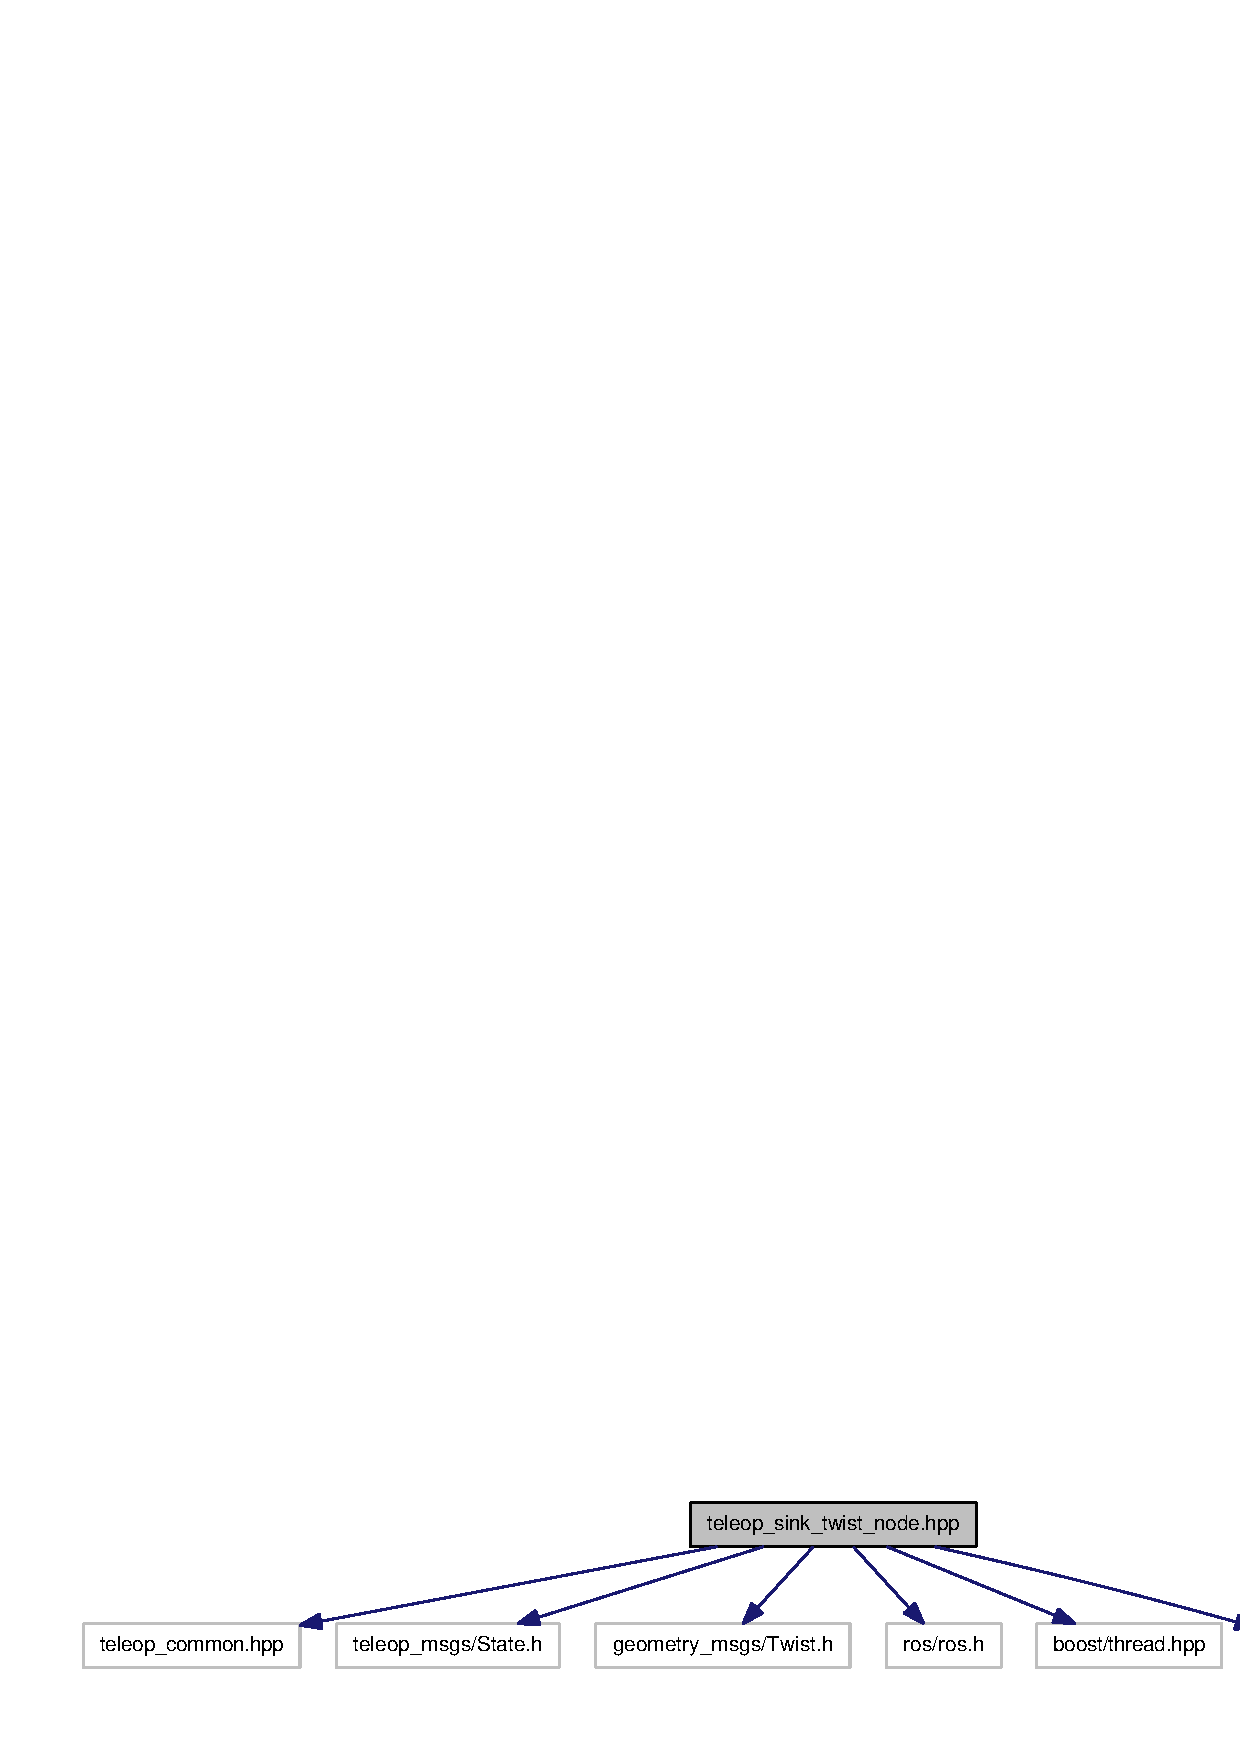
\includegraphics[width=400pt]{teleop__sink__twist__node_8hpp__incl}
\end{center}
\end{figure}
This graph shows which files directly or indirectly include this file:
\nopagebreak
\begin{figure}[H]
\begin{center}
\leavevmode
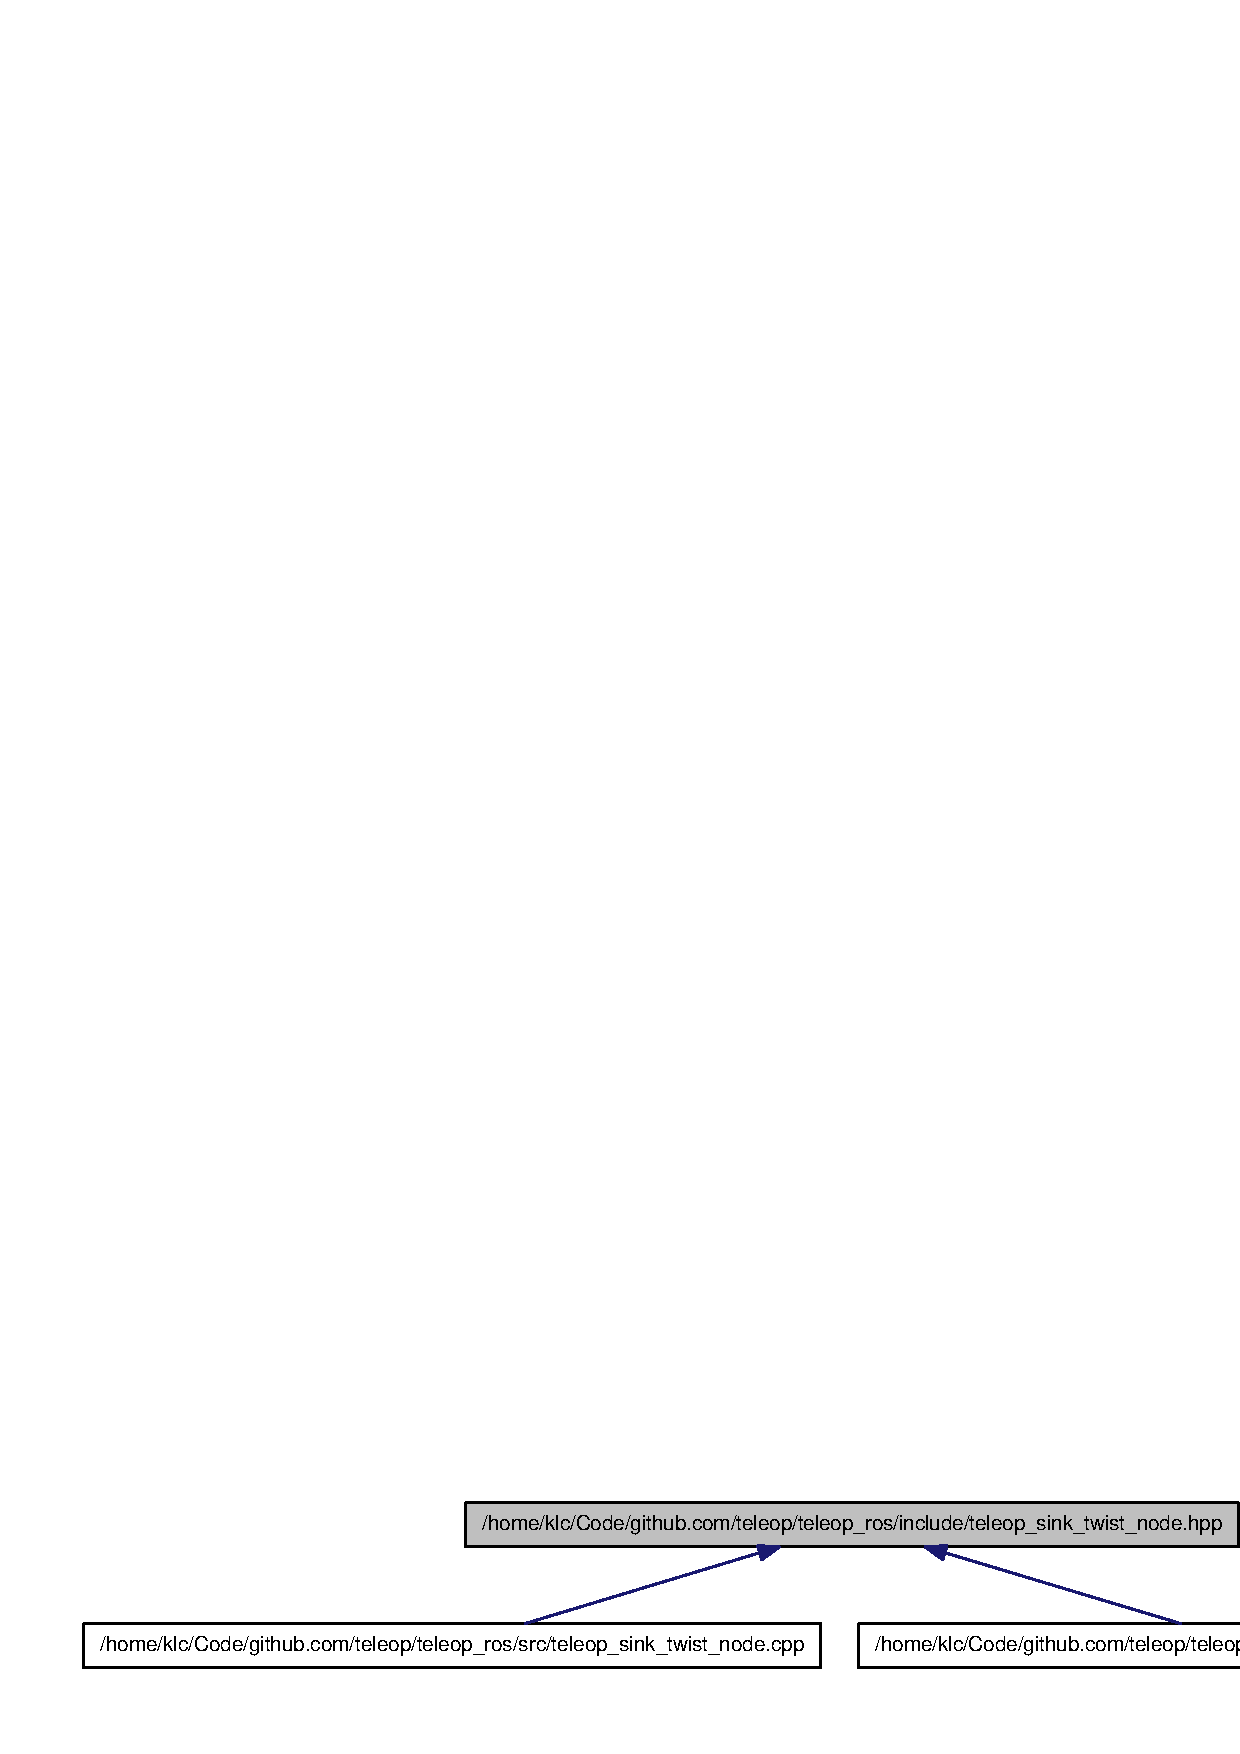
\includegraphics[width=400pt]{teleop__sink__twist__node_8hpp__dep__incl}
\end{center}
\end{figure}
\subsection*{Classes}
\begin{DoxyCompactItemize}
\item 
class {\bf teleop::TeleopSinkTwistNode}
\end{DoxyCompactItemize}
\subsection*{Namespaces}
\begin{DoxyCompactItemize}
\item 
namespace {\bf teleop}
\end{DoxyCompactItemize}

\section{/home/klc/Code/github.com/teleop/teleop\_\-ros/include/teleop\_\-source\_\-node.hpp File Reference}
\label{teleop__source__node_8hpp}\index{/home/klc/Code/github.com/teleop/teleop\_\-ros/include/teleop\_\-source\_\-node.hpp@{/home/klc/Code/github.com/teleop/teleop\_\-ros/include/teleop\_\-source\_\-node.hpp}}
{\ttfamily \#include $<$teleop\_\-common.hpp$>$}\par
{\ttfamily \#include $<$teleop\_\-source.hpp$>$}\par
{\ttfamily \#include $<$teleop\_\-source\_\-adapter.hpp$>$}\par
{\ttfamily \#include $<$teleop\_\-msgs/State.h$>$}\par
{\ttfamily \#include $<$ros/ros.h$>$}\par
{\ttfamily \#include $<$boost/thread.hpp$>$}\par
{\ttfamily \#include $<$stdint.h$>$}\par
Include dependency graph for teleop\_\-source\_\-node.hpp:
\nopagebreak
\begin{figure}[H]
\begin{center}
\leavevmode
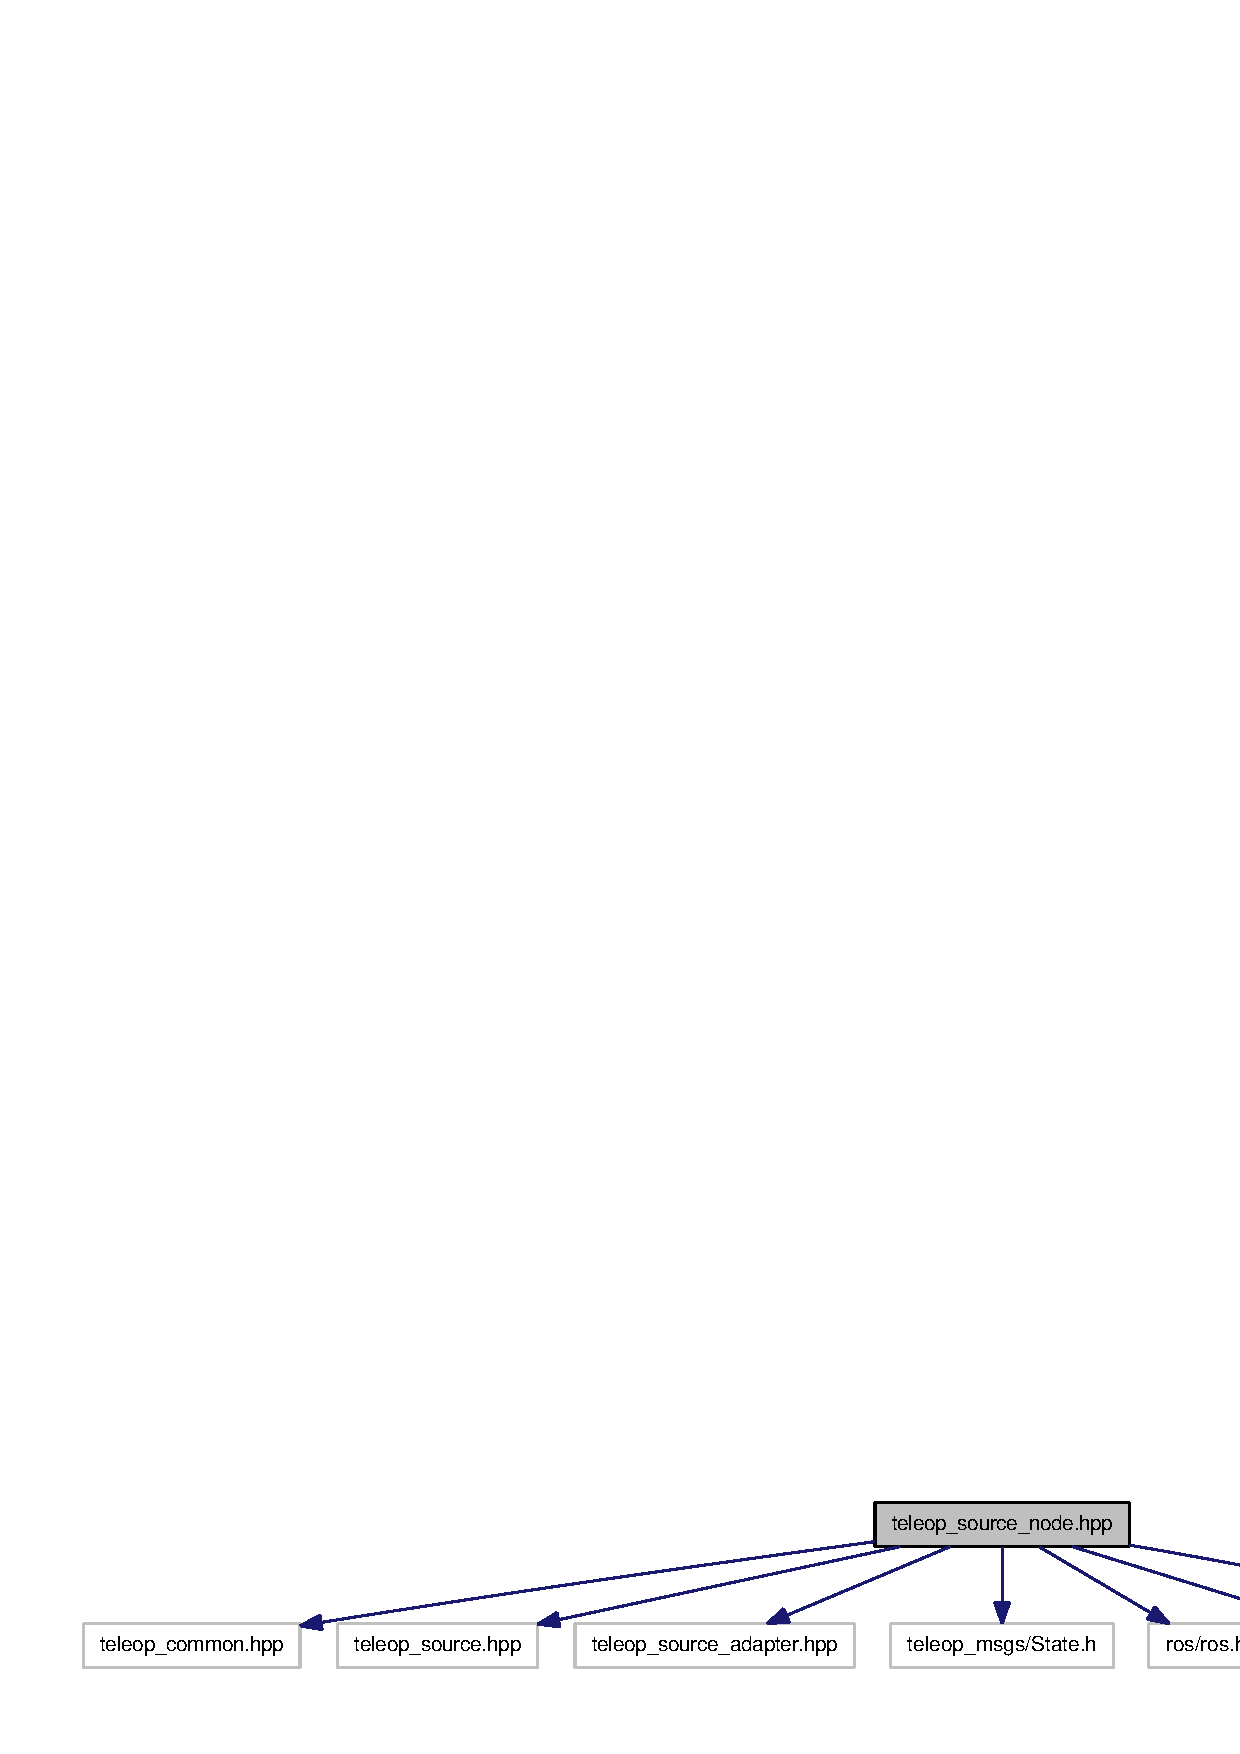
\includegraphics[width=400pt]{teleop__source__node_8hpp__incl}
\end{center}
\end{figure}
This graph shows which files directly or indirectly include this file:
\nopagebreak
\begin{figure}[H]
\begin{center}
\leavevmode
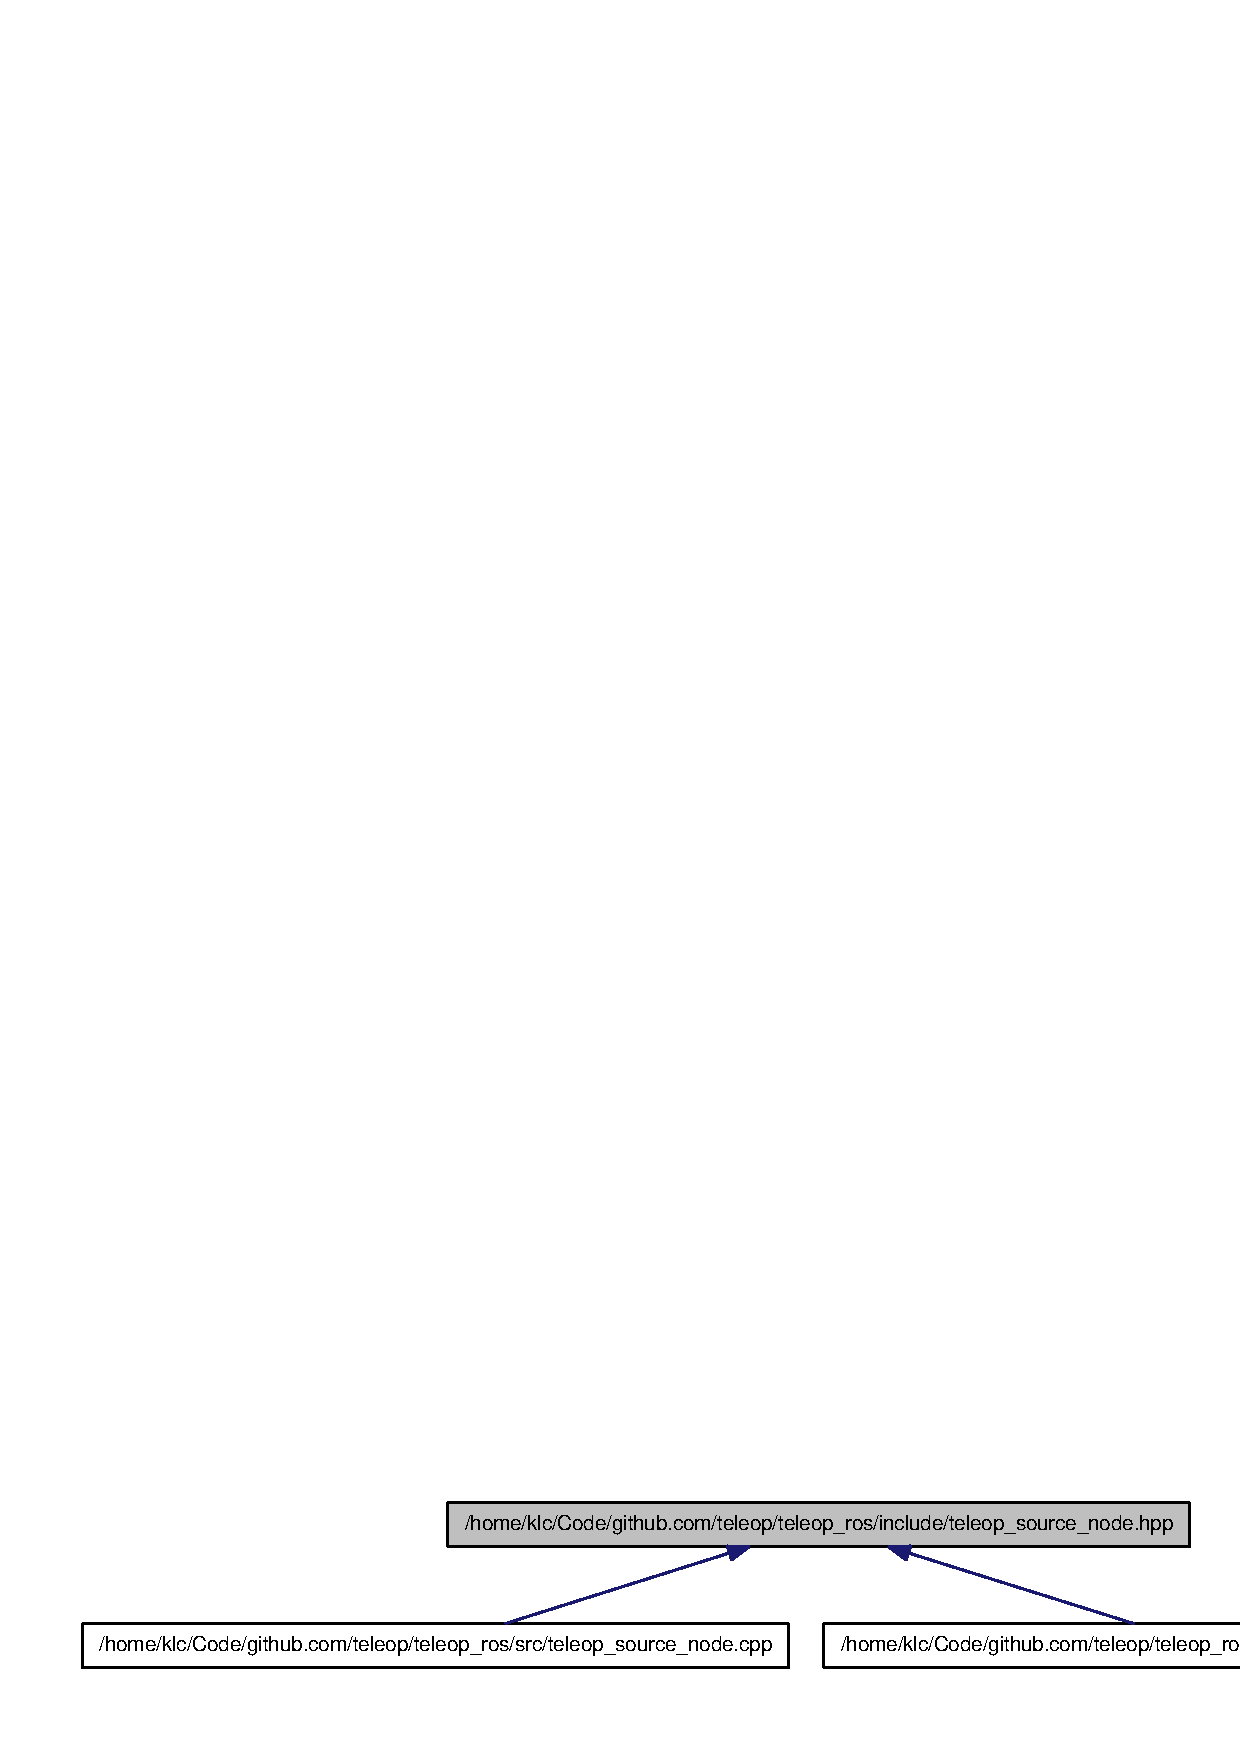
\includegraphics[width=400pt]{teleop__source__node_8hpp__dep__incl}
\end{center}
\end{figure}
\subsection*{Classes}
\begin{DoxyCompactItemize}
\item 
class {\bf teleop::TeleopSourceNode}
\end{DoxyCompactItemize}
\subsection*{Namespaces}
\begin{DoxyCompactItemize}
\item 
namespace {\bf teleop}
\end{DoxyCompactItemize}

\section{/home/klc/Code/github.com/teleop/teleop\_\-msgs/mainpage.dox File Reference}
\label{mainpage_8dox}\index{/home/klc/Code/github.com/teleop/teleop\_\-msgs/mainpage.dox@{/home/klc/Code/github.com/teleop/teleop\_\-msgs/mainpage.dox}}

\section{/home/klc/Code/github.com/teleop/teleop\_\-ros/src/teleop\_\-sink\_\-twist\_\-node.cpp File Reference}
\label{teleop__sink__twist__node_8cpp}\index{/home/klc/Code/github.com/teleop/teleop\_\-ros/src/teleop\_\-sink\_\-twist\_\-node.cpp@{/home/klc/Code/github.com/teleop/teleop\_\-ros/src/teleop\_\-sink\_\-twist\_\-node.cpp}}
{\ttfamily \#include $<$teleop\_\-common.hpp$>$}\par
{\ttfamily \#include $<$teleop\_\-msgs/State.h$>$}\par
{\ttfamily \#include $<$geometry\_\-msgs/Twist.h$>$}\par
{\ttfamily \#include $<$ros/ros.h$>$}\par
{\ttfamily \#include $<$boost/thread.hpp$>$}\par
{\ttfamily \#include $<$stdint.h$>$}\par
{\ttfamily \#include $<$signal.h$>$}\par
{\ttfamily \#include $<$stdio.h$>$}\par
Include dependency graph for teleop\_\-sink\_\-twist\_\-node.cpp:
\nopagebreak
\begin{figure}[H]
\begin{center}
\leavevmode
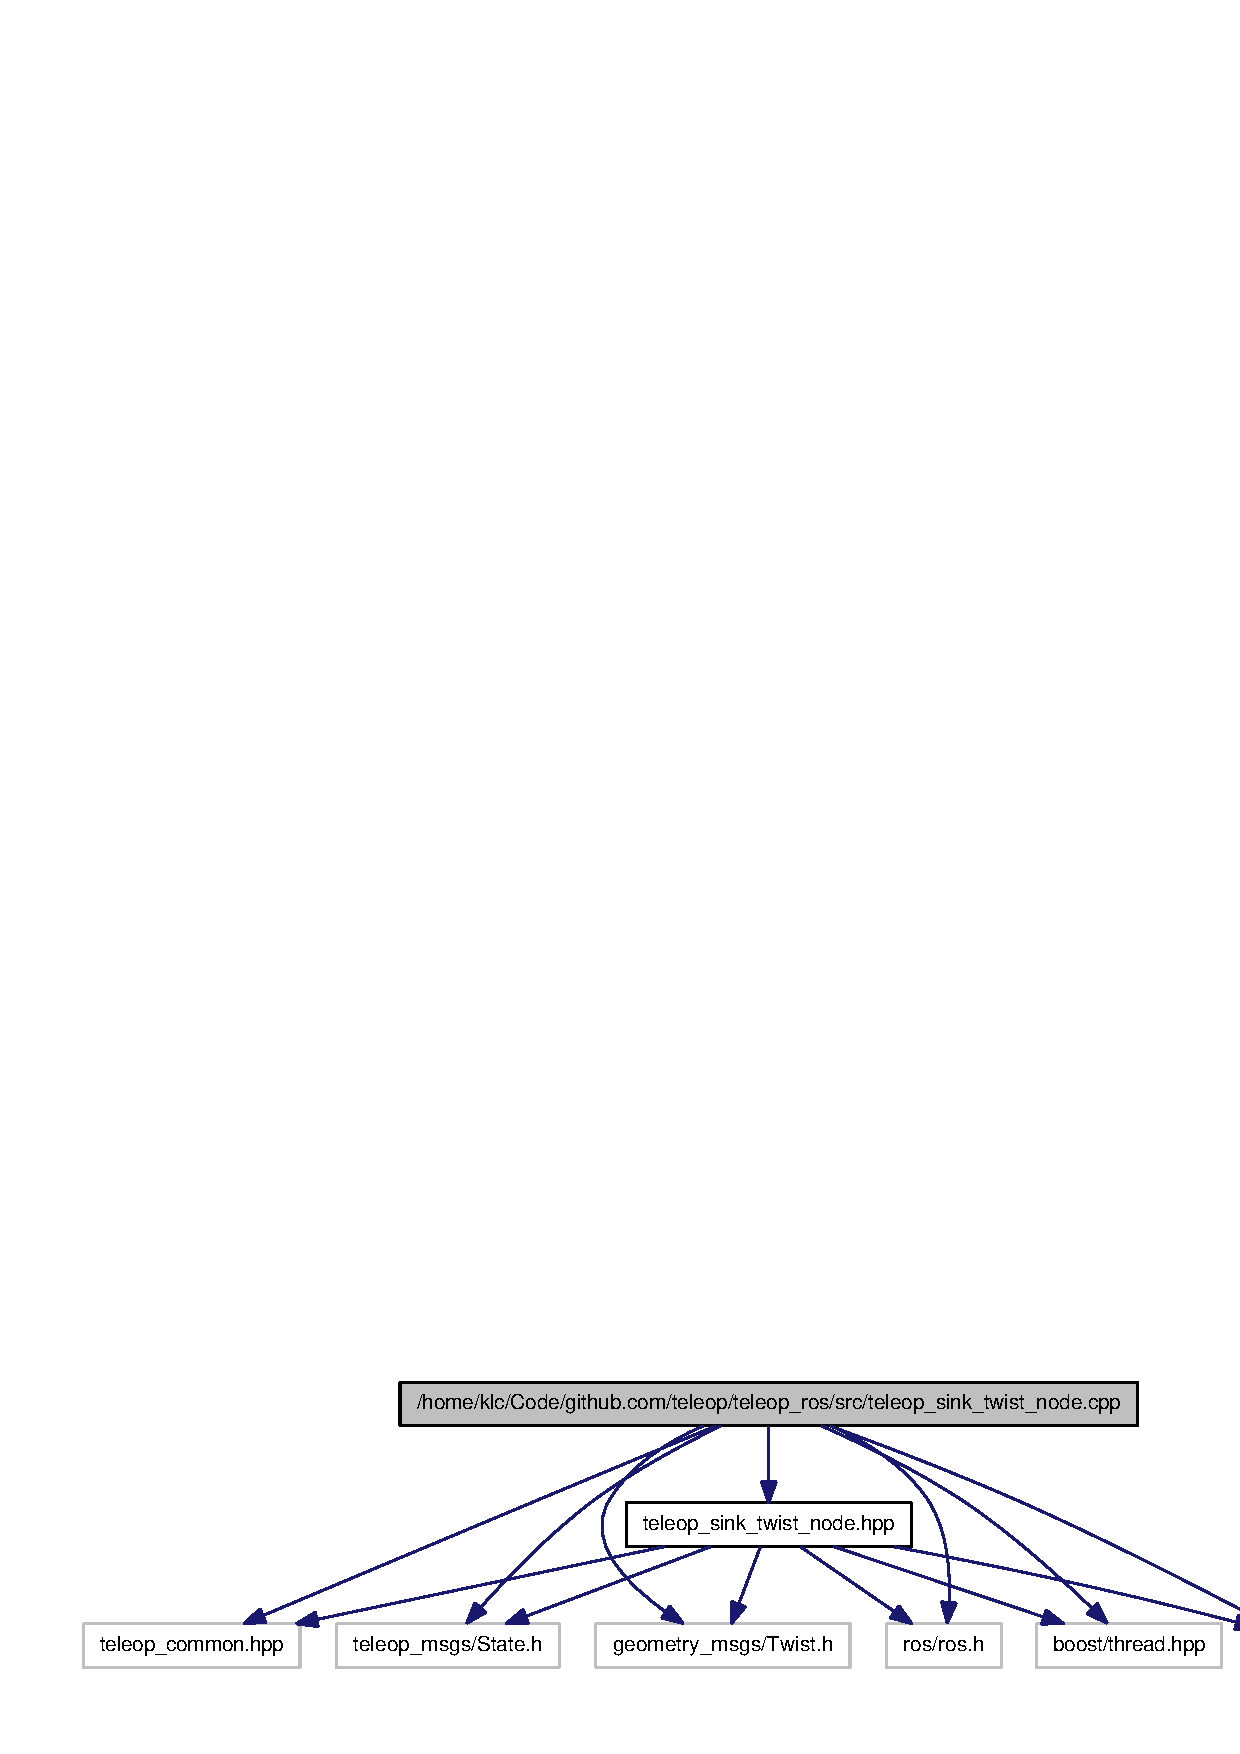
\includegraphics[width=400pt]{teleop__sink__twist__node_8cpp__incl}
\end{center}
\end{figure}
\subsection*{Functions}
\begin{DoxyCompactItemize}
\item 
int {\bf main} (int argc, char $\ast$$\ast$argv)
\end{DoxyCompactItemize}


\subsection{Function Documentation}
\index{teleop\_\-sink\_\-twist\_\-node.cpp@{teleop\_\-sink\_\-twist\_\-node.cpp}!main@{main}}
\index{main@{main}!teleop_sink_twist_node.cpp@{teleop\_\-sink\_\-twist\_\-node.cpp}}
\subsubsection[{main}]{\setlength{\rightskip}{0pt plus 5cm}int main (
\begin{DoxyParamCaption}
\item[{int}]{argc, }
\item[{char $\ast$$\ast$}]{argv}
\end{DoxyParamCaption}
)}\label{teleop__sink__twist__node_8cpp_a3c04138a5bfe5d72780bb7e82a18e627}


Definition at line 976 of file teleop\_\-sink\_\-twist\_\-node.cpp.


\section{/home/klc/Code/github.com/teleop/teleop\_\-ros/src/teleop\_\-sink\_\-twist\_\-node\_\-main.cpp File Reference}
\label{teleop__sink__twist__node__main_8cpp}\index{/home/klc/Code/github.com/teleop/teleop\_\-ros/src/teleop\_\-sink\_\-twist\_\-node\_\-main.cpp@{/home/klc/Code/github.com/teleop/teleop\_\-ros/src/teleop\_\-sink\_\-twist\_\-node\_\-main.cpp}}
{\ttfamily \#include $<$teleop\_\-sink\_\-twist\_\-node.hpp$>$}\par
{\ttfamily \#include $<$ros/ros.h$>$}\par
{\ttfamily \#include $<$boost/thread.hpp$>$}\par
{\ttfamily \#include $<$signal.h$>$}\par
{\ttfamily \#include $<$string.h$>$}\par
{\ttfamily \#include $<$stdio.h$>$}\par
Include dependency graph for teleop\_\-sink\_\-twist\_\-node\_\-main.cpp:
\nopagebreak
\begin{figure}[H]
\begin{center}
\leavevmode
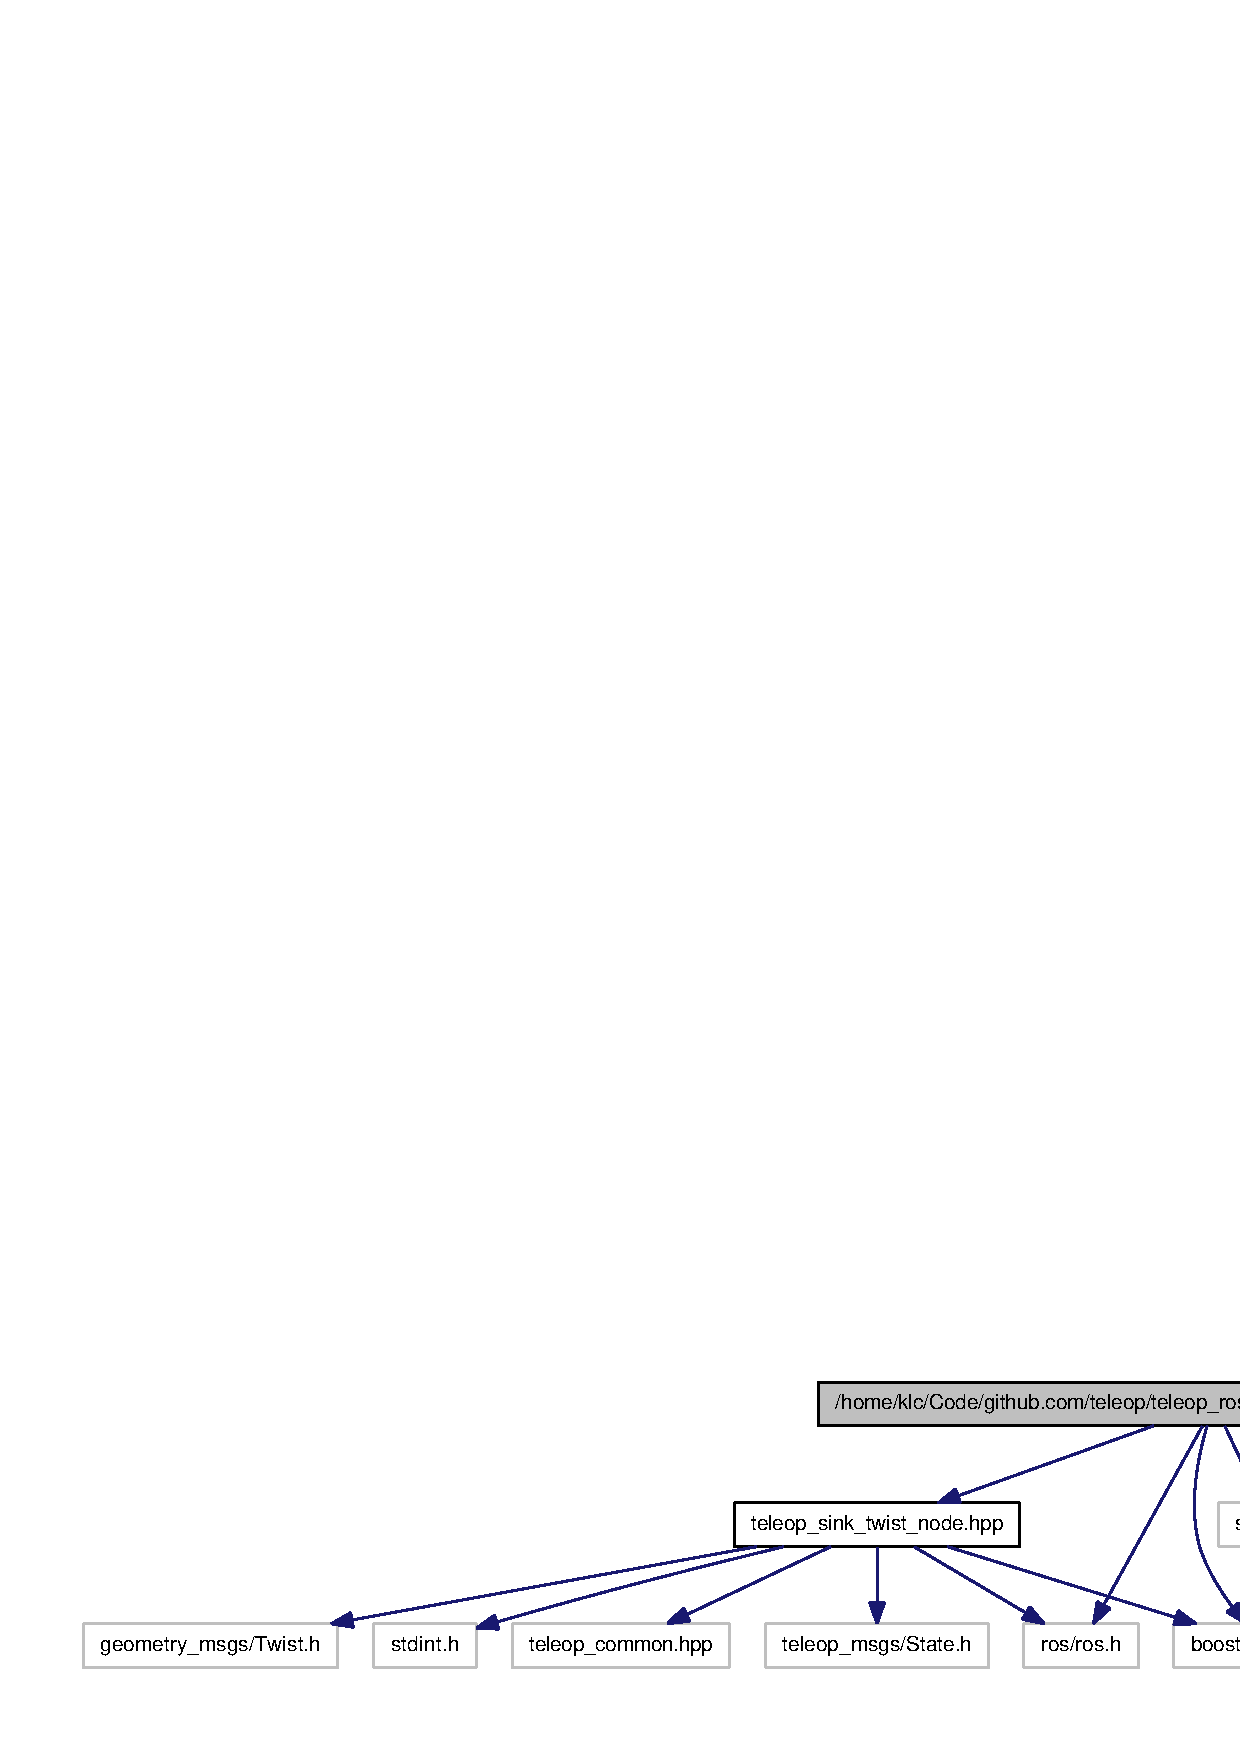
\includegraphics[width=400pt]{teleop__sink__twist__node__main_8cpp__incl}
\end{center}
\end{figure}
\subsection*{Functions}
\begin{DoxyCompactItemize}
\item 
int {\bf main} (int argc, char $\ast$$\ast$argv)
\item 
static bool {\bf printUsage} (std::string nodeName, int argc, char $\ast$$\ast$argv)
\item 
static void {\bf signalHandler} (int signalNumber)
\end{DoxyCompactItemize}
\subsection*{Variables}
\begin{DoxyCompactItemize}
\item 
static sig\_\-atomic\_\-t {\bf gInterruptRequested} = 0
\end{DoxyCompactItemize}


\subsection{Function Documentation}
\index{teleop\_\-sink\_\-twist\_\-node\_\-main.cpp@{teleop\_\-sink\_\-twist\_\-node\_\-main.cpp}!main@{main}}
\index{main@{main}!teleop_sink_twist_node_main.cpp@{teleop\_\-sink\_\-twist\_\-node\_\-main.cpp}}
\subsubsection[{main}]{\setlength{\rightskip}{0pt plus 5cm}int main (
\begin{DoxyParamCaption}
\item[{int}]{argc, }
\item[{char $\ast$$\ast$}]{argv}
\end{DoxyParamCaption}
)}\label{teleop__sink__twist__node__main_8cpp_a3c04138a5bfe5d72780bb7e82a18e627}


Definition at line 203 of file teleop\_\-sink\_\-twist\_\-node\_\-main.cpp.

\index{teleop\_\-sink\_\-twist\_\-node\_\-main.cpp@{teleop\_\-sink\_\-twist\_\-node\_\-main.cpp}!printUsage@{printUsage}}
\index{printUsage@{printUsage}!teleop_sink_twist_node_main.cpp@{teleop\_\-sink\_\-twist\_\-node\_\-main.cpp}}
\subsubsection[{printUsage}]{\setlength{\rightskip}{0pt plus 5cm}static bool printUsage (
\begin{DoxyParamCaption}
\item[{std::string}]{nodeName, }
\item[{int}]{argc, }
\item[{char $\ast$$\ast$}]{argv}
\end{DoxyParamCaption}
)\hspace{0.3cm}{\ttfamily  [static]}}\label{teleop__sink__twist__node__main_8cpp_a45a08ffb90ada6472f08f092b6a403f4}
Check if we should just print usage information, and if so, print it.


\begin{DoxyParams}{Parameters}
{\em nodeName} & [in] -\/ node name \\
\hline
{\em argc} & [in] -\/ number of command line arguments \\
\hline
{\em argv} & [in] -\/ command line arguments\\
\hline
\end{DoxyParams}
\begin{DoxyReturn}{Returns}
true if usage was printed 
\end{DoxyReturn}


Definition at line 84 of file teleop\_\-sink\_\-twist\_\-node\_\-main.cpp.

\index{teleop\_\-sink\_\-twist\_\-node\_\-main.cpp@{teleop\_\-sink\_\-twist\_\-node\_\-main.cpp}!signalHandler@{signalHandler}}
\index{signalHandler@{signalHandler}!teleop_sink_twist_node_main.cpp@{teleop\_\-sink\_\-twist\_\-node\_\-main.cpp}}
\subsubsection[{signalHandler}]{\setlength{\rightskip}{0pt plus 5cm}static void signalHandler (
\begin{DoxyParamCaption}
\item[{int}]{signalNumber}
\end{DoxyParamCaption}
)\hspace{0.3cm}{\ttfamily  [static]}}\label{teleop__sink__twist__node__main_8cpp_af7cb763a339a6219a80607a4947b9f5f}
Signal handler.


\begin{DoxyParams}{Parameters}
{\em signalNumber} & [in] -\/ received signal number \\
\hline
\end{DoxyParams}


Definition at line 80 of file teleop\_\-sink\_\-twist\_\-node\_\-main.cpp.



\subsection{Variable Documentation}
\index{teleop\_\-sink\_\-twist\_\-node\_\-main.cpp@{teleop\_\-sink\_\-twist\_\-node\_\-main.cpp}!gInterruptRequested@{gInterruptRequested}}
\index{gInterruptRequested@{gInterruptRequested}!teleop_sink_twist_node_main.cpp@{teleop\_\-sink\_\-twist\_\-node\_\-main.cpp}}
\subsubsection[{gInterruptRequested}]{\setlength{\rightskip}{0pt plus 5cm}sig\_\-atomic\_\-t {\bf gInterruptRequested} = 0\hspace{0.3cm}{\ttfamily  [static]}}\label{teleop__sink__twist__node__main_8cpp_a22bc7c017fbdfd918e67984d16126658}
Global atomic flag used to indicate if an interrupt has been requested. 

Definition at line 72 of file teleop\_\-sink\_\-twist\_\-node\_\-main.cpp.


\section{teleop\_\-source\_\-node.cpp File Reference}
\label{teleop__source__node_8cpp}\index{teleop\_\-source\_\-node.cpp@{teleop\_\-source\_\-node.cpp}}
{\ttfamily \#include $<$teleop\_\-source\_\-node.hpp$>$}\par
{\ttfamily \#include $<$teleop\_\-common.hpp$>$}\par
{\ttfamily \#include $<$teleop\_\-source.hpp$>$}\par
{\ttfamily \#include $<$teleop\_\-source\_\-adapter.hpp$>$}\par
{\ttfamily \#include $<$teleop\_\-source\_\-keyboard.hpp$>$}\par
{\ttfamily \#include $<$teleop\_\-source\_\-joystick.hpp$>$}\par
{\ttfamily \#include $<$teleop\_\-msgs/State.h$>$}\par
{\ttfamily \#include $<$ros/ros.h$>$}\par
{\ttfamily \#include $<$boost/thread.hpp$>$}\par
{\ttfamily \#include $<$stdint.h$>$}\par
Include dependency graph for teleop\_\-source\_\-node.cpp:
\nopagebreak
\begin{figure}[H]
\begin{center}
\leavevmode
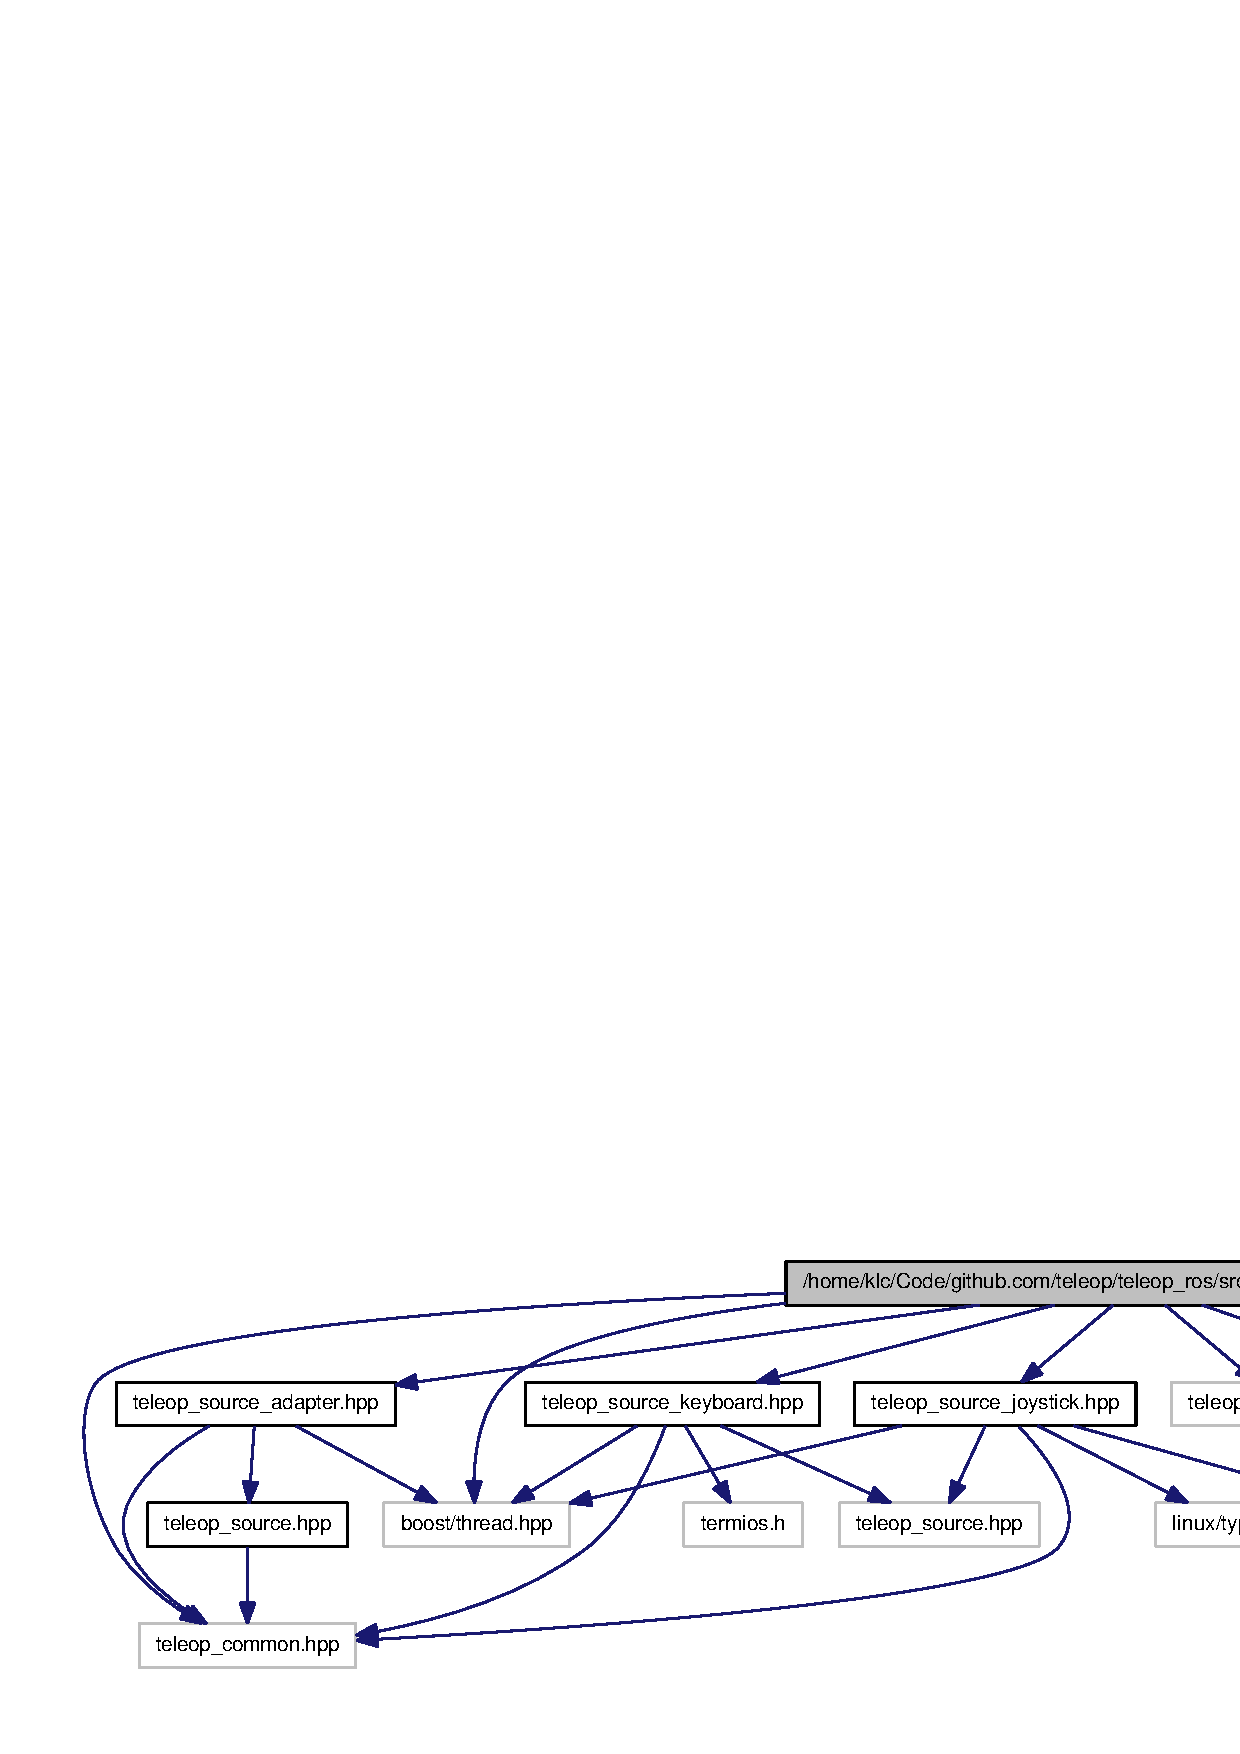
\includegraphics[width=400pt]{teleop__source__node_8cpp__incl}
\end{center}
\end{figure}
\subsection*{Namespaces}
\begin{DoxyCompactItemize}
\item 
namespace {\bf teleop}
\end{DoxyCompactItemize}

\section{/home/klc/Code/github.com/teleop/teleop\_\-ros/src/teleop\_\-source\_\-node\_\-main.cpp File Reference}
\label{teleop__source__node__main_8cpp}\index{/home/klc/Code/github.com/teleop/teleop\_\-ros/src/teleop\_\-source\_\-node\_\-main.cpp@{/home/klc/Code/github.com/teleop/teleop\_\-ros/src/teleop\_\-source\_\-node\_\-main.cpp}}
{\ttfamily \#include $<$teleop\_\-source\_\-node.hpp$>$}\par
{\ttfamily \#include $<$ros/ros.h$>$}\par
{\ttfamily \#include $<$boost/thread.hpp$>$}\par
{\ttfamily \#include $<$signal.h$>$}\par
{\ttfamily \#include $<$string.h$>$}\par
{\ttfamily \#include $<$stdio.h$>$}\par
Include dependency graph for teleop\_\-source\_\-node\_\-main.cpp:
\nopagebreak
\begin{figure}[H]
\begin{center}
\leavevmode
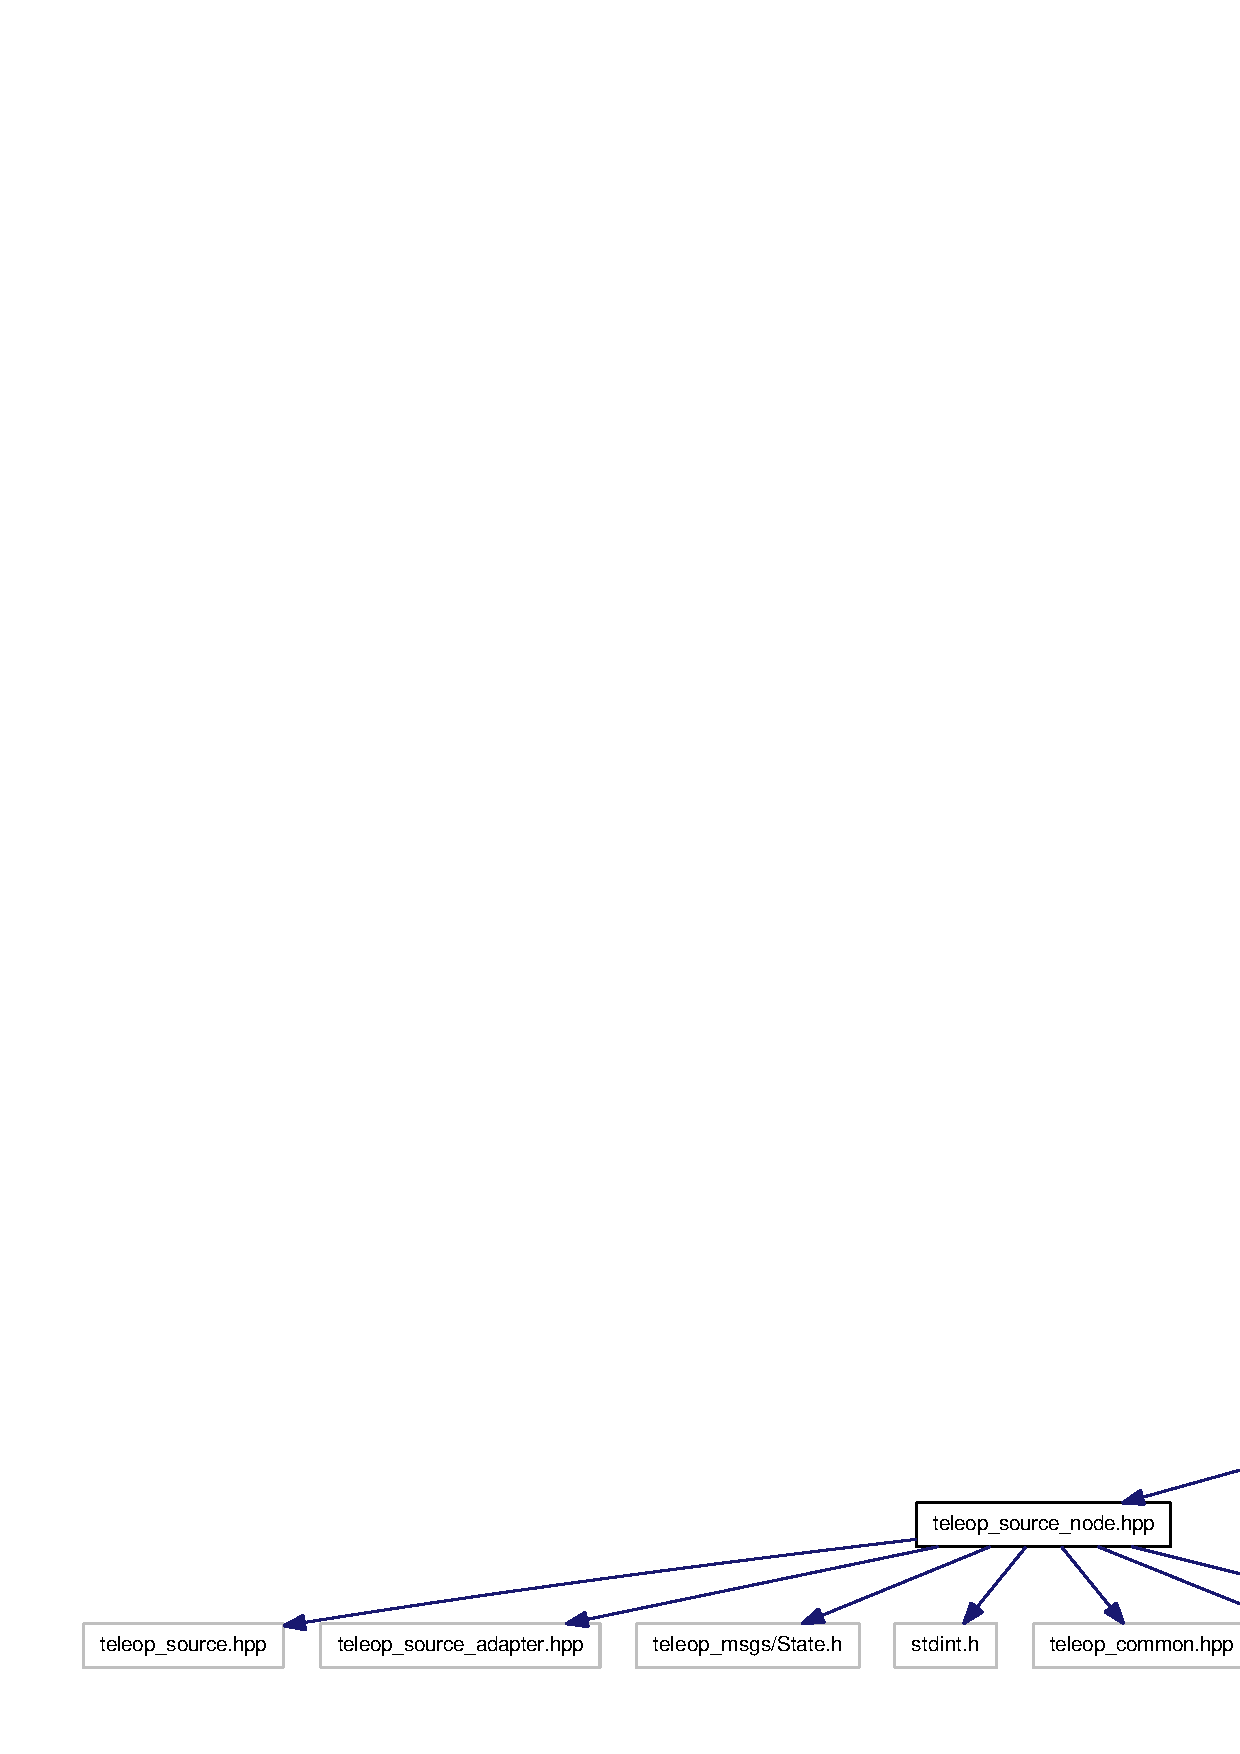
\includegraphics[width=400pt]{teleop__source__node__main_8cpp__incl}
\end{center}
\end{figure}
\subsection*{Functions}
\begin{DoxyCompactItemize}
\item 
int {\bf main} (int argc, char $\ast$$\ast$argv)
\item 
static bool {\bf printUsage} (std::string nodeName, int argc, char $\ast$$\ast$argv)
\item 
static void {\bf signalHandler} (int signalNumber)
\end{DoxyCompactItemize}
\subsection*{Variables}
\begin{DoxyCompactItemize}
\item 
static sig\_\-atomic\_\-t {\bf gInterruptRequested} = 0
\end{DoxyCompactItemize}


\subsection{Function Documentation}
\index{teleop\_\-source\_\-node\_\-main.cpp@{teleop\_\-source\_\-node\_\-main.cpp}!main@{main}}
\index{main@{main}!teleop_source_node_main.cpp@{teleop\_\-source\_\-node\_\-main.cpp}}
\subsubsection[{main}]{\setlength{\rightskip}{0pt plus 5cm}int main (
\begin{DoxyParamCaption}
\item[{int}]{argc, }
\item[{char $\ast$$\ast$}]{argv}
\end{DoxyParamCaption}
)}\label{teleop__source__node__main_8cpp_a3c04138a5bfe5d72780bb7e82a18e627}


Definition at line 125 of file teleop\_\-source\_\-node\_\-main.cpp.

\index{teleop\_\-source\_\-node\_\-main.cpp@{teleop\_\-source\_\-node\_\-main.cpp}!printUsage@{printUsage}}
\index{printUsage@{printUsage}!teleop_source_node_main.cpp@{teleop\_\-source\_\-node\_\-main.cpp}}
\subsubsection[{printUsage}]{\setlength{\rightskip}{0pt plus 5cm}static bool printUsage (
\begin{DoxyParamCaption}
\item[{std::string}]{nodeName, }
\item[{int}]{argc, }
\item[{char $\ast$$\ast$}]{argv}
\end{DoxyParamCaption}
)\hspace{0.3cm}{\ttfamily  [static]}}\label{teleop__source__node__main_8cpp_a45a08ffb90ada6472f08f092b6a403f4}
Check if we should just print usage information, and if so, print it.


\begin{DoxyParams}{Parameters}
{\em nodeName} & [in] -\/ node name \\
\hline
{\em argc} & [in] -\/ number of command line arguments \\
\hline
{\em argv} & [in] -\/ command line arguments\\
\hline
\end{DoxyParams}
\begin{DoxyReturn}{Returns}
true if usage was printed 
\end{DoxyReturn}


Definition at line 84 of file teleop\_\-source\_\-node\_\-main.cpp.

\index{teleop\_\-source\_\-node\_\-main.cpp@{teleop\_\-source\_\-node\_\-main.cpp}!signalHandler@{signalHandler}}
\index{signalHandler@{signalHandler}!teleop_source_node_main.cpp@{teleop\_\-source\_\-node\_\-main.cpp}}
\subsubsection[{signalHandler}]{\setlength{\rightskip}{0pt plus 5cm}static void signalHandler (
\begin{DoxyParamCaption}
\item[{int}]{signalNumber}
\end{DoxyParamCaption}
)\hspace{0.3cm}{\ttfamily  [static]}}\label{teleop__source__node__main_8cpp_af7cb763a339a6219a80607a4947b9f5f}
Signal handler.


\begin{DoxyParams}{Parameters}
{\em signalNumber} & [in] -\/ received signal number \\
\hline
\end{DoxyParams}


Definition at line 80 of file teleop\_\-source\_\-node\_\-main.cpp.



\subsection{Variable Documentation}
\index{teleop\_\-source\_\-node\_\-main.cpp@{teleop\_\-source\_\-node\_\-main.cpp}!gInterruptRequested@{gInterruptRequested}}
\index{gInterruptRequested@{gInterruptRequested}!teleop_source_node_main.cpp@{teleop\_\-source\_\-node\_\-main.cpp}}
\subsubsection[{gInterruptRequested}]{\setlength{\rightskip}{0pt plus 5cm}sig\_\-atomic\_\-t {\bf gInterruptRequested} = 0\hspace{0.3cm}{\ttfamily  [static]}}\label{teleop__source__node__main_8cpp_a22bc7c017fbdfd918e67984d16126658}
Global atomic flag used to indicate if an interrupt has been requested. 

Definition at line 72 of file teleop\_\-source\_\-node\_\-main.cpp.


\printindex
\end{document}
